%----------------------------------------------------------------------------------
% Exemplo do uso da classe pucrs-ppgcc.cls. Veja o arquivo .cls
% para mais detalhes e instruções.
%----------------------------------------------------------------------------------

% Seleção de idioma da monografia. Por enquanto as únicas opções
% suportadas são 'portuguese' e 'english'
% Para impressão em frente e verso, use a opção 'twoside'. Da
% mesma forma, use 'oneside' para impressão em um lado apenas.
%\documentclass[portuguese,twoside]{pucrs-ppgcc}
% \documentclass[english,twoside]{pucrs-ppgcc}
\documentclass[english]{pucrs-ppgcc}

%----------------------------------------------------------------
% Coloque seus pacotes abaixo.
%
% Obs.: muitos pacotes de uso comum do LaTeX, como amsmath,
% geometry e url já são automaticamente incluídos pela classe
% (veja o arquivo .cls). Isso torna obrigatória a presença destes
% no sistema para o uso desta classe, mas ao mesmo tempo o uso se
% torna mais simples.  Recomendo a instalação da versão mais
% recente da distribuição TeXLive (para Windows e UNIXes):
% www.tug.org/texlive/
%
% Pacotes e opções já incluídas automaticamente:
%
% \RequirePackage[T1]{fontenc}[2005/09/27]
% \RequirePackage[utf8x]{inputenc}[2008/03/30]
% \RequirePackage[english,brazil]{babel}[2008/07/06]
% \RequirePackage[a4paper]{geometry}[2010/09/12]
% \RequirePackage{textcomp}[2005/09/27]
% \RequirePackage{lmodern}[2009/10/30]
% \RequirePackage{indentfirst}[1995/11/23]
% \RequirePackage{setspace}[2000/12/01]
% \RequirePackage{textcase}[2004/10/07]
% \RequirePackage{float}[2001/11/08]
% \RequirePackage{amsmath}[2000/07/18]
% \RequirePackage{amssymb}[2009/06/22]
% \RequirePackage{amsfonts}[2009/06/22]
% \RequirePackage{url}
% \RequirePackage[table]{xcolor}[2007/01/21]
%\RequirePackage{array}[2008/09/09]
%\RequirePackage{longtable}
%----------------------------------------------------------------
% Para inserção de figuras.
\usepackage{graphicx}
\usepackage{subcaption}
\captionsetup{compatibility=false}
% Utilize a opção 'pdftex' se você estiver usando o pdflatex (que
% permite figuras em formatos como .jpg ou .png)
%\usepackage[pdftex]{graphicx}

\usepackage{booktabs}
% Para tabelas com elementos ocupando mais de uma linha
\usepackage{multirow}
% Para frações na mesma linha (ex. ⅓).
\usepackage{nicefrac}
% Para inserir figuras lado a lado.
% \usepackage{subfigure}
% Para formatar algoritmos.
% A opção [algo2e] é necessária para evitar conflitos
% com as definições da classe.
%\usepackage[algo2e]{algorithm2e}
\usepackage{algorithmic}
% Um float do tipo algoritmo. No momento
% este pacote é incompatível com a classe.
%\usepackage{algorithm}
% acronyms
\usepackage{acronym}

% pretty beautiful latex table
% \documentclass{article}
\usepackage{tabu}
\usepackage{longtable}
\usepackage[table]{xcolor}
\definecolor{tableHeader}{RGB}{0, 200, 200}
\definecolor{tableLineOne}{RGB}{245, 245, 245}
\definecolor{tableLineTwo}{RGB}{224, 224, 224}
\newcommand{\tableHeaderStyle}{
    \rowfont{\leavevmode\color{white}\bfseries}
    \rowcolor{tableHeader}
}

\usepackage{mathtools,amssymb}
\usepackage{booktabs, isotope,colortbl,caption}

\arrayrulecolor{cyan}
% \captionsetup[table]{labelfont={color=cyan,sc},justification=RaggedRight,singlelinecheck=false,skip=2pt}

\newlength{\mytablewidth}
\newsavebox{\mytablebox}

 \renewcommand{\arraystretch}{1.5}

\hypersetup{
    colorlinks = true,
    allcolors = blue
}

\setcounter{secnumdepth}{5}

%----------------------------------------------------------------
% Autor (OBRIGATÓRIO)
%----------------------------------------------------------------
\author{\small{Darlan Alves Jurak}}

%----------------------------------------------------------------
% Título (OBRIGATÓRIO). Devem ser passados DOIS parâmetros,
% o título em português E o inglês, não importando o idioma
% escolhido. Os títulos são utilizados para a montagem da capa,
% resumo e abstract mais tarde.
%----------------------------------------------------------------
\newcommand{\writeTitleHere}{a \acs{COLREGS}-compliant guidance system for unmanned surface vehicles}
% \newcommand{\writeTitleHere}{A COLREGs Compliant Collision Avoidance System for Unmanned Surface Vehicles}
\newcommand{\writeTitleHerePT}{Um Sistema de Orientação para Veículos Não-Tripulados que Navegam na Superfície da Água com Respeito à COLREGs}

\title{\writeTitleHerePT}
      {\writeTitleHere}

%----------------------------------------------------------------
% Opções para o tipo de trabalho (OBRIGATÓRIO)
%----------------------------------------------------------------
% \tipotrabalho{\pep}   % Monografias em geral (e de "bônus": TCCs)
%\tipotrabalho{\pep}         % Plano de estudo e pesquisa
\tipotrabalho{\dissertacao} % Dissertação
%\tipotrabalho{\ptese}       % Proposta de tese
%\tipotrabalho{\tese}        % Tese

%----------------------------------------------------------------
% Seleção do curso ("este trabalho é um requisito parcial para
% obtenção do grau de (mestre ou doutor) em Ciência da Computação").
% Necessário somente para o tipo 'monografia'.
%----------------------------------------------------------------
%\grau{\bacharel} % Este é "bônus"
\grau{\mestre}
%\grau{\doutor}

%----------------------------------------------------------------
% Orientador (e Co-orientador, caso haja um). É OBRIGATÓRIO
% informar pelo menos o orientador.
%----------------------------------------------------------------
\orientador{Alexandre de Morais Amory}
\coorientador{Vitor Augusto Machado Jorge}

%----------------------------------------------------------------
% Commom text
%----------------------------------------------------------------
\newcommand{\ie}{{\it i.e.}}
\newcommand{\eg}{{\it e.g.}}
\newcommand{\etc}{{\it etc.}}
\newcommand{\etal}{{\it et al.}}
\newcommand{\usvsim}{{USVsim}}

%----------------------------------------------------------------
% TODOs
%----------------------------------------------------------------

\usepackage{lipsum}                     % Dummytext
\usepackage{xargs}                      % Use more than one optional parameter in a new commands

%----------------------------------------------------------------
% PDF
%----------------------------------------------------------------
\usepackage{pdfpages}

%----------------------------------------------------------------
% Appendice
%----------------------------------------------------------------
\usepackage[toc,page]{appendix}

%----------------------------------------------------------------
% Landscape
%----------------------------------------------------------------
\usepackage{lscape}

% 
\usepackage[colorinlistoftodos,prependcaption,textsize=tiny]{todonotes}
\newcommandx{\unsure}[2][1=]{\todo[linecolor=red,backgroundcolor=red!25,bordercolor=red,#1]{#2}}
\newcommandx{\change}[2][1=]{\todo[linecolor=blue,backgroundcolor=blue!25,bordercolor=blue,#1]{#2}}
\newcommandx{\info}[2][1=]{\todo[linecolor=OliveGreen,backgroundcolor=OliveGreen!25,bordercolor=OliveGreen,#1]{#2}}
\newcommandx{\improvement}[2][1=]{\todo[linecolor=Plum,backgroundcolor=Plum!25,bordercolor=Plum,#1]{#2}}
\newcommandx{\thiswillnotshow}[2][1=]{\todo[disable,#1]{#2}}

%----------------------------------------------------------------
% A capa é inserida automaticamente. Por isso não é necessário
% chamar \maketitle
%----------------------------------------------------------------
\begin{document}

%----------------------------------------------------------------
% Depois da capa vem a dedicatória e a epígrafe.
%----------------------------------------------------------------
%\dedicatoria{Dedico este trabalho a meus pais.}

%\epigrafe{The art of simplicity is a puzzle of complexity.}{Douglas Horton}

%----------------------------------------------------------------
% Também dá para fazer as duas na mesma página:
%----------------------------------------------------------------
%\dedigrafe{Dedico este trabalho a meus pais.}
%          {The art of simplicity is a puzzle of complexity.}
%          {Douglas Horton}

%----------------------------------------------------------------
% A seguir, a página de agradecimentos (OPCIONAL):
%----------------------------------------------------------------
%\begin{agradecimentos}
%À lorem ipsum, dolor sit amet consetetur sadipscing elitr sed diam nonumy eirmod tempor. invidunt ut labore et dolore magna aliquyam
%\end{agradecimentos}

%----------------------------------------------------------------
% Resumo, com as palavras-chave passadas por parâmetro
% (OBRIGATÓRIO, ao menos para teses e dissertações)
%----------------------------------------------------------------
%\begin{resumo}{lorem, ipsum, dolor, sit, amet}
%Seu resumo em português aqui. lorem ipsum dolor sit amet consetetur sadipscing elitr sed diam nonumy eirmod tempor invidunt ut labore et dolore magna aliquyam erat sed diam voluptua at vero eos et accusam et justo duo dolores et ea rebum stet clita.  kasd gubergren no sea takimata sanctus est lorem ipsum dolor sit amet lorem ipsum dolor sit amet consetetur sadipscing elitr sed diam nonumy eirmod tempor invidunt ut labore et dolore magna aliquyam erat sed diam voluptua at.
%\end{resumo}

%----------------------------------------------------------------
% Abstract, com as palavras-chave passadas por parâmetro
% (OBRIGATÓRIO, ao menos para teses e dissertações)
%----------------------------------------------------------------
%\begin{abstract}{lorem, ipsum, dolor, sit, amet}
%Your abstract in English here. lorem ipsum dolor sit amet consetetur sadipscing elitr sed diam nonumy eirmod tempor invidunt ut labore et dolore magna aliquyam erat sed diam voluptua at vero eos et accusam et justo duo dolores et ea rebum stet clita kasd gubergren no sea takimata sanctus est lorem ipsum dolor sit amet lorem ipsum dolor sit amet consetetur sadipscing elitr sed diam nonumy eirmod tempor invidunt ut labore et dolore magna aliquyam erat sed diam voluptua at
%\end{abstract}

%----------------------------------------------------------------
% Listas e sumário, nessa ordem. Somente o sumário é obrigatório,
% portanto, comente as outras listas, caso sejam desnecessárias.
%----------------------------------------------------------------
%\listoffigures       % Lista de figuras      (OPCIONAL)
%\listoftables        % Lista de tabelas      (OPCIONAL)
%\listofalgorithms    % Lista de algoritmos   (OPCIONAL)
%\listofacronyms      % Lista de siglas       (OPCIONAL)
%\listofabbreviations % Lista de abreviaturas (OPCIONAL)
%\listofsymbols       % Lista de símbolos     (OPCIONAL)
\setcounter{tocdepth}{1}
\tableofcontents     % Sumário               (OBRIGATÓRIO)

%----------------------------------------------------------------
% Aqui começa o desenvolvimento do trabalho. Para uma melhor
% organização do documento, separe-o em arquivos,
% um para cada capítulo. Para isso, utilize o comando \include,
% como mostrado abaixo.
%----------------------------------------------------------------
\begin{acronym}
\acro{AIS}      {Automatic Identification System}
\acro{ARPA}     {Automatic Radar Plotting Aid}
\acro{ATC}      {Artificial Terrain Cost}
\acro{EV}       {Encountering Vessel}
\acro{COA}      {Circle of Acceptance}
\acro{COR}      {Circle of Rejection}
\acro{CPA}      {Closest Point of Approach}
\acro{COLREGS}  {Convention on the International Regulations for Preventing Collisions at Sea}
\acro{DGPS}     {Differential Global Positioning System}
\acro{DPSS}     {Direction Priority Sequential Selection}
\acro{GNC}      {Guidance, Navigation and Control}
\acro{GP}       {Genetic Programming}
\acro{GPS}      {Global Positioning System}
\acro{GUI}      {Graphical User Interface}
\acro{HTN}      {Hierarchical Task Network}
\acro{IMO}      {International Marine Organization}
\acro{JSHOP}    {Java Simple Hierarchical Ordered Planner}
\acro{LADAR}    {Laser Radar}
\acro{LIDAR}    {Light Detection and Ranging}
\acro{LOS}      {Line of Sight}
\acro{LSA}      {Autonomous System Laboratory}
\acro{MPC}      {Model Predictive Control}
\acro{MVFF}     {Modified Virtual Force Field}
\acro{MWR}      {Milimeter Wave Radar}
\acro{NORMAM}   {\textit{Normas da Autoridade Marítima}}
\acro{ODE}      {Ordinary Differential Equation}
\acro{OV}       {Own Vessel}
\acro{PEP}      {Research Plan}
\acro{PID}      {Proportional–Integral–Derivative}
\acro{POC}      {Proof-of-Concept}
\acro{RGBD}     {Red-Green-Blue-Depth}
\acro{ROS}      {Robotic Operating System}
\acro{R-RA*}    {Rule-based Repairing A*}
\acro{SA}       {\textit{Seminário de Andamento}}
\acro{SONAR}    {Sound Navigation and Ranging}
\acro{TSS}      {Traffic Separation Schemes}
\acro{USV}      {Unmanned Surface Vehicle}
\acro{VFF}      {Virtual Force Field}
\acro{VO}       {Velocity Obstacle}
% \acrodefplural{OS}[OS's]{Operating Systems}
\end{acronym}
\chapter{Introduction \label{chap:intro}}

    %%%%%%%%%%%%%%%%%%
    % Grammarly:99/100
    %%%%%%%%%%%%%%%%%%
    
    % General Context    
    Approximately 71\% of the Earth is covered by water, and essential tasks happen on its surface, such as environment monitoring, merchandising, and exploration. Some of these tasks can be dangerous, exhaustive, or tedious for humans, so a trend is the development of autonomous systems for executing these tasks. Thus, driven by military, scientific, and commercial interests, the development of \acp{USV} has become a current demand \cite{Liu2016Unmanned}.
    
    % Definition of USV
    \acp{USV} constitute a category of marine robots that act without a crew on the water surface, presenting autonomous behavior or being remotely controlled. In the last decades, several techniques have been applied for making \acp{USV} autonomous. The main challenges are related to collision avoidance, precise navigation on the seagoing, and accordance with international marine rules, namely \ac{COLREGS}.
    Current \ac{USV} applications include: environment monitoring \cite{Caccia2005Sampling}; ocean resources exploration as oil and gas exploration \cite{Pastore2010Improving}; port, harbor and coastal surveillance for military purposes \cite{Caccia2007unmanned, Pastore2010Improving, Svec2011aAutomated}; transportation \cite{Kiencke2005Impact}; and scientific research \cite{Yan2010Development}.
    
    % Collision Avoidance
    % The \acs{COLREGS} determines rules that must be followed by maritime pilots for preventing collisions in potential collision scenarios such as crossing, head-on, and overtaking. Currently, a direct collision between ships represents 60\% of the accidents in the sea, and 56\% of the collisions are caused by \acs{COLREGS} violation \cite{Liu2016Unmanned, Campbell2012Review_COLREGs}. Thus, \ac{USV} must be compliant with the \ac{COLREGS} rules, but the fact that \ac{COLREGS} were written by humans to humans using subjective and ambiguous terms generated dependency on human interpretation, implying a considerable challenge for \acp{USV} systems.
    The \acs{COLREGS} determines rules that must be followed by maritime pilots for preventing collisions in potential collision scenarios such as crossing, head-on, and overtaking. Currently, direct collision between ships represents 60\% of the accidents at sea, and 56\% of the collisions are caused by \acs{COLREGS} violation \cite{Liu2016Unmanned, Campbell2012Review_COLREGs}. Thus, \acp{USV} must be compliant with the \ac{COLREGS}.
    
    % Proposed work
    % In this dissertation, we present a \ac{COLREGS}-compliant \ac{USV} system capable of avoiding collision with static and dynamic obstacles. We developed COLREGS compliance integrating the creation of virtual obstacles that block not COLREGS-compliant regions in the search space used by the path planner. We used \ac{ROS} for implementation\cite{Quigley2009ROS} while the evaluation of the system's behavior is done through software simulation using the USV\_sim simulator \cite{Paravisi2018Toward}.% and on field tests using the Platypus Lutra airboat \cite{PlatypusLutraAirboat}. 
    
    \section{Research Problem and Scope}
    
    %%%%%%%%%%%%%%%%%%
    % Grammarly:?/100
    %%%%%%%%%%%%%%%%%%
    
    \ac{USV} \ac{COLREGS} compliant systems already exist and are being developed extensively. We note that many works on \ac{USV} have the proposal of developing specific applications with \ac{USV} and sometimes end up not providing access to their applications, or are protected with patents. In our laboratory, we have small unmanned vessels with the potential to be used in disaster situations during the monitoring phase or in activities to collect water samples for quality assessment. The focus of this work is to generate a system that can serve as a basis for the autonomous guidance of our vessels. As respect for the international rules of the navy is of high relevance, we chose to develop the base system with \ac{COLREGS} compliance.
    
    Our scope is in simulation, we developed and validated our system using the USV\_sim\footnote{https://github.com/disaster-robotics-proalertas/usv\_sim\_lsa}~\cite{Paravisi2018Toward} simulator.
    %AMA bota o link tb
    The USV\_sim is a simulator developed by our research group, which besides allowing simulation considering realistic disturbances such as wind influence, also has realistic representations of the vessels that we have in our research group. For the development of our system, we use the \ac{ROS}~\cite{Quigley2009ROS} framework that is widely used around the world, and we believe this way, we can continue to develop our system in a distributed and collaborative way.
    
    % \section{Goals}
    
    % The goal of this work is to provide a COLREGS-compliant \ac{USV} system. Considering distributed and collaborative development we developed the core of our COLREGS-compliant system as a ROS plugin. Moreover, we integrated the COLREGS-compliant USV system to the USV\_sim simulator.
    
    \section{Contributions}
    
    %%%%%%%%%%%%%%%%%%
    % Grammarly:99/100
    %%%%%%%%%%%%%%%%%%
    
     Our main contribution is a \ac{COLREGS}-compliant \ac{USV} system capable of avoiding collision with static and dynamic obstacles. We developed our system under the \ac{ROS} framework to enable collaborative and distributed development. Also, we make the COLREGS-compliant path planner of our system available as a \ac{ROS} plugin\footnote{https://github.com/Unmanned-Surface-Vehicle/atc\_astar}. Furthermore, regarding the evaluation of our system, we integrated it into the USV\_sim simulator. This integration allowed us to evaluate our system considering realistic environmental disturbances such as wind influence. Our system can be used as a base system for further development.

    \section{Publications}
    
    During the master's period, the author has a journal article and two papers accepted for publication. We summarize the contributions presented in each already accepted publication as follows.
    
    %AMA para cada artigo. diga onde foi publicado. coloca uma ref em cada um
    \begin{enumerate}
        \item 2019
            \begin{itemize}
                \item "A Survey on Unmanned Surface Vehicles for Disaster Robotics: Main Challenges and Directions" \cite{Jorge2019Survey}. This paper presents the first comprehensive survey about the applications and roles of \acp{USV} for disaster management, to the best of our knowledge. Currently, we have 11 citations around the world.
                \item "Programming teaching with robotic support for people who are visually impaired: a systematic review" \cite{Damasio2019Programming}. In our laboratory, we developed a robotic environment composed of programming language, simulation, and a robot to aid people who are visually impaired to learn programming. In this paper, we extended a review of other works that aid visually impaired people on learning programming with robotics.
                \item "Integrating an MPSoC to a Robotics Environment \cite{Domingues2019Integrating}. In this work, we integrated a \ac{MPSoC} and a robotic simulator and ran a trivial application for demonstration purposes.
            \end{itemize}
    \end{enumerate}
    
    \section{Thesis Outline}
    
    % Thesis Outline
    In Chapter \ref{chap:2_TheoreticalBackground}, we present important definitions and background information related to our research. In Chapter \ref{chap:3_LiteratureReview}, we present and discuss the literature related to \acp{USV} guidance systems. 
    In Chapter \ref{chap:4_COLREGS_Compliant_Guidance_System}, we present the developed system, its architecture and features. In Chapter \ref{chap:5_Simulation_And_Results}, we present simulation scenarios and results. In Chapter \ref{chap:6_Conclusion}, we discuss the collected results.
    
\chapter{Theoretical Background \label{chap:2_TheoreticalBackground}}


    In this chapter we present some background on the main concepts related to our study. The focus is to define the guidance components of a \ac{USV}, and present the international regulations for navigation of vessels on water (\acs{COLREGS}).

\section{GNC System}
    
    The \acs{GNC} system is essential component for most \acp{USV}, being responsible for manage partially or entirely the \ac{USV}. GNC stands for Guidance, Navigation, and Control being composed of software and onboard computers. In this section, we describe the responsibilities of each one of these modules as well as the interaction between them.
    
    \subsection{Guidance System}

    In an autonomous approach, most \acp{USV} guidance systems are responsible for planning the path that will be traveled by the \ac{USV} using available information about static and dynamic obstacles captured by the navigation and the perception system.

    In general, trajectory generation shall be in accordance with the \ac{USV} mission and marine protocols, such as being in accordance with the \ac{COLREGS} or respect \ac{TSS} definitions\footnote{\ac{TSS} are similar to traffic ground lines that must be respected by vessels on navigation at sea.}. Also, information about vehicle capability and environmental conditions may be required to determine suitable trajectories.
    
    % Gloabl path-planning algorithms evaluate the whole information available on a certain area in order to generate an obstacle-free path between the departure location, or initial waypoint, and the destination, or final waypoint. Candeloro2017Voronoi
    As presented in Chapter \ref{chap:3_LiteratureReview}, typical implementations of the guidance system propose the usage of global and local guidance modules. Thus, the global guidance module becomes responsible for path planning related to the far-field based on well-known information about the environment and assuming a deliberative behavior. Conversely, the local guidance module is responsible for path planning related to the near-field environment, assuming a reactive behavior. Both global and local guidance systems usually define the \ac{USV} trajectory considering static and dynamic obstacles.
    
    In general, static information about the environment such as islands, boulders, etc, is extracted from nautical charts and topography maps. While dynamic information about the environment is acquired in runtime sensing by the perception system and through real-time updated electronic navigation charts capable of identifying other vessels and obstacles. Moreover, the guidance system depends on a world representation (e.g., 2D/3D maps representation, and occupancy grids) for running its main component, the path planner. Conventional methods for path planning applied to \ac{USV} guidance are optimization methods based on evolutionary algorithm and heuristics methods.
    % VJ Acho que o parágrafo esta com informação faltando. O runtime sensing usando o perception system é uma coisa e a eletronic navigation chart é outra.  Separe cada uma delas e suas funções. "real-time updated electronic navigation charts" não é um tipo de world representation? Vc menciona o perception system aqui e na sessão abaixo. Me parece que deveria estar em outro lugar ou mais elaborado aqui.
    % DJ: Partially done: acredito ter corrigido de maneira adequada a parte referente à "runtime sensing" mas o resto fiquei com duvidas e optei por seguir em frente e deixar assim por enquanto.

    \subsection{Navigation, Control and Perception systems}
    
    The navigation system is responsible by the \ac{USV} current state estimation (i.e., position, velocity, orientation, and acceleration) and measurement of some environment information (e.g., wind speed and ocean current), being composed of \acs{GPS}, compasses, and barometers. 
    The control system is responsible for keeping the actuators of the \ac{USV} following the trajectory generated by the guidance system. 
    Moreover, lately, studies present the perception system as a central component of a \ac{USV} together with guidance, navigation, and control systems. 
    % VJ frase perdida e repetida anteriormente?
    % DJ: N concordo.
    In general, perception systems are composed of cameras and near-field range sensors such as \ac{LIDAR}.
    Figure \ref{fig:Liu2016Unmanned_GNCSystem} presented by Liu \etal~\cite{Liu2016Unmanned} shows a big picture of the \ac{GNC} system, the responsibilities of each module and the interaction between them, elucidating the definitions presented in this section. 
    
    \begin{figure}[H]
        \centering
        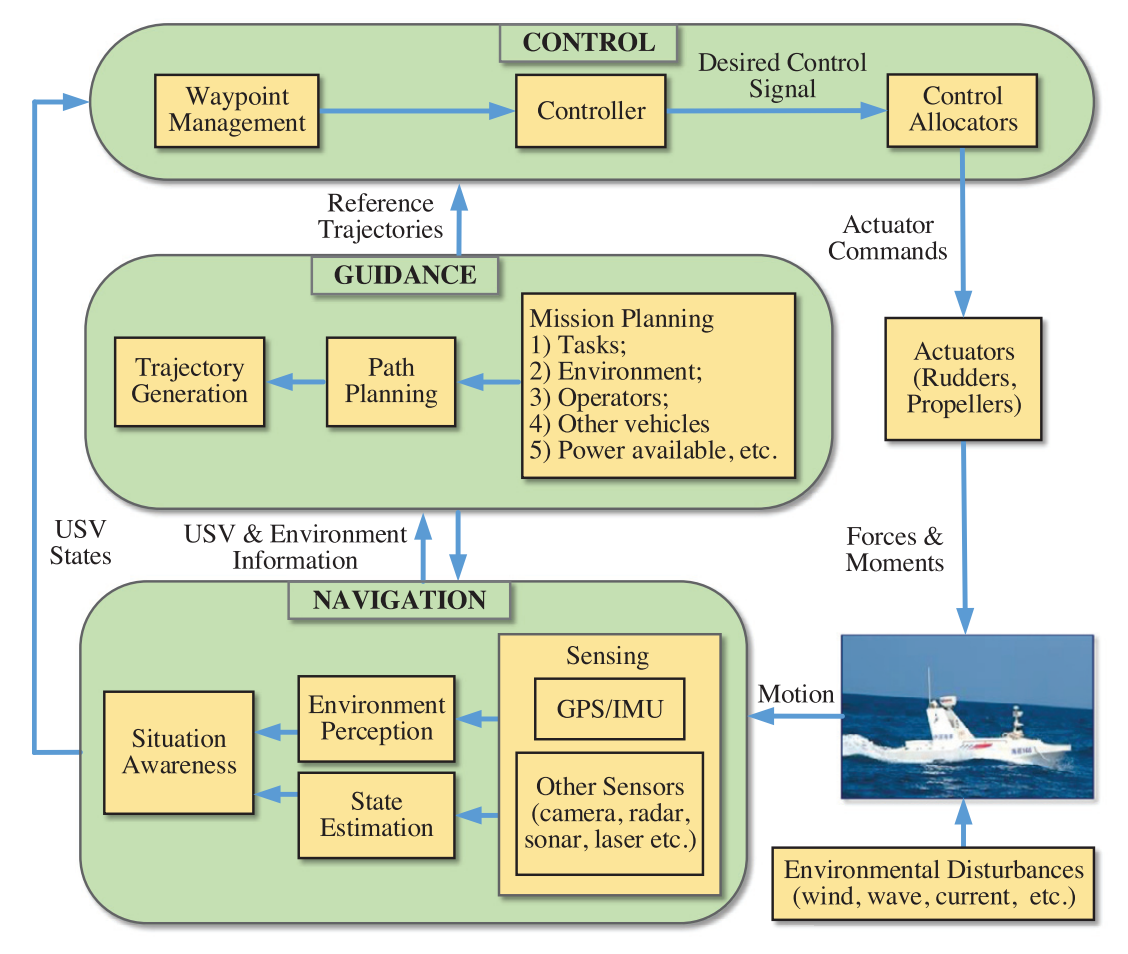
\includegraphics[scale=0.7]{figs/Chap2/Liu2016Unmanned_GNCSystem.png}
        \caption{\ac{GNC} System - Components and interaction between them \cite{Liu2016Unmanned}}
        \label{fig:Liu2016Unmanned_GNCSystem}
    \end{figure}
    
    % VJ o que é importante na imagem? O que vc quer que o leitor saiba? Apontar na label e no texto. Lemre-se que vc não tem direito autoral das imagens e que isso pode virar uma dor de cabeça se o autor for chato. Sempre consulte os autores ao usar imagens de terceiros.
    
    % \subsubsection{Behavior-based systems}
        
        %% Benjamin2004COLREGS
        % The origin of behavior-based systems is commonly attributed to Brooks' "subsumption architecture" in [R. Brooks, “A Robust Layered Control System for a Mobile Robot”, IEEE Journal of Robofics and Automation, RA-2(1):14-23, April 1986]. Since then, it has been used in a large variety of applications including: indoor robots, e.g., [l, 2, 7, 9, 13, 14, 17, 19, 201, land vehicles, e.g., [16], planetary rovers, e.g., [12, 181, and marine vehicles, e.g., [3,4,6,8, 15] 
        
        %% Benjamin2004COLREGS
        % Action selection, as indicated in Fig. 1, is the process of choosing a single action for execution, given the outputs of the behaviors. The "action space" is the set of all possible distinct actions, e.g., all speed, heading and depth combinations for a marine vehicle.
        
        %% Benjamin2004COLREGS
        % Its influence depends on whether the rule associated with the behavior applies to the current situation. The output of each behavior is an objective function that rates all possible actions with respect to the corresponding COLREGS rule. The detaiIs of solving multi-objective optimization problems in the interval programming model can be found in [3]
        
    % \subsubsection{Genetic Programming}
    % Genetic Programming is an automated programming technique, based on the automated composition of 
    % a set of functional programming blocks into an increasing amount of modules for 
    % generation of a structured solution with the desired functionality. 
    % Genetic Programming explore a random combination of functional blocks through the generation of expressions 
    % tree where each node is represents a functional block. Solutions are generated by combination, mutation and
    % crossover between subtrees.
    
    % \subsubsection{A*}
    
    % The A* algorithm is a classical grid-based methodology which has been widely applied in different shapes and forms. It uses s heuristic method to focus the search towards the goal position. Using an edge cost and a heuristic based on the Euclidean distance, the A* algorithm can find the shortest paths \cite{Hart1972Formal}. For the classical A* algorithm, its scalability is limited by its memory requirements. It stores all explored nodes of a search graph in the memory, using an Open List to store nodes on the search frontier and a Closed List to store already-expanded nodes.
    
    % Depending on the size of the grid map, a large number of nodes may have to be searched at any given time. Thus, repeatedly searching through these lists can slow down the application significantly. Hence, it is not suitable for real-time engineering applications requiring on-the-fly computations.
    
    % Search space
    
    % \subsubsection{Occupancy Grid}
    % \subsubsection{Velocity Obstacle} \unsure[inline]{maybe remove from here and explain only in the literature review}
    
    % The velocity obstacle (VO) approach has been adopted by several researchers for moving hazard avoidance. Since it was first proposed in 1998 for robot motion planning [10], several extensions to VO have been made.  VO approaches generate a cone-shaped obstacle in the velocity space (hence the name velocity obstacles) and ensure that there will be no future collisions as long as the robot’s velocity vector is outside the VO. To identify the risk of future collisions, one could predict both the pose of the moving hazard and the pose of the robot for several time steps into the future, and perform collision checks using their configurations at each time slice. This approach has the advantage that it can check collisions of vehicles following arbitrary trajectories. However, because it needs to perform collision checks at many time slices, the computational load becomes very high.

    % On the other hand, VO makes a first-order (i.e., linear) prediction, and the collision check is done in the velocity space. Since a single collision check accounts for collision checks at all future times (due to the linear velocity assumption), VO is very fast to compute and extends well to high-speed operations with short reaction time. Furthermore, its simplicity is suited for our behavior-based control architecture.
    
    % \subsubsection{Line of Sight}
    % \subsubsection{Direction Priority Sequential Selection} \unsure[inline]{maybe remove from here and explain only in the literature review}
    % \subsubsection{Rule-Rapairing A*} \unsure[inline]{maybe remove from here and explain only in the literature review}
    % \subsubsection{Virtual Force Field}
    % \subsubsection{Fuzzy Logic}
    % \subsubsection{Interval Programming}
    % \subsubsection{Closest Point of Approach}
        % One is using various indicators to measure a collision risk and find associated evasive actions that keep the risk at an acceptable level. Two widely used indicators, Distance to CPA (DCPA) and Time to CPA (TCPA), are based on the concept of closest point of approach (CPA) (Kearon, 1979).
    % \subsubsection{Occupancy Grid}

\section{COLREGS}
\label{sec:colregs}

    %Campbell2012Rule
    % Human error, both active and latent, are said to cause marine collisions in an estimated 89-96\% of cases (Roth-blum (2000)), for instance the catastrophic MVDo˜na Paz ferry collision with the MTVector. An intelligent Obstacle Detection and Avoidance (ODA) system can potentially eliminate the issues caused by poor judgement or failure to react promptly.

    \ac{COLREGS}\cite{COLREGS} stands for “International Regulation for Preventing Collisions at Sea, 1972”, sometimes cited as "COLlision REGulations at Sea" or "Convention on the International Regulations for Preventing Collisions at Sea" -- in this work we adopted the latter. The definitions declared on the \ac{COLREGS} are controlled, updated and of responsibility of the \ac{IMO}. Briefly, the \ac{COLREGS} defines the rules that must be followed by vessels upon waters to avoid collision. 
    The \ac{COLREGS} are adopted by the United Nations as a global convention and must be respected by every country.
    
    The \ac{COLREGS} include 41 rules divided into five sections: General document appliance, Steering \& Sailing, Lights \& Shapes, Sound and Light Signals, and Exceptions. Relevant rules in the context of the present work are listed below. For purpose of discussion we underline subjective or ambiguous terms:
    % VJ: Em português criamos frases gigantes, em Inglês, evite isso e quebre frases que vão ficar muito grandes sempre que possível. O termo no-objective acho que se escreve sem hífen e significa: emotional; based on inner experience rather than fact. Subjective. Vc não deve usar plural ali. 
    % DJ: "Non-objective" removed.
    % Paragraph reduced.
    
    \begin{itemize}
    % VJ: penso eu que seja visto como plágio um número tão elevado de frases citadas exatamente como são. Talvez fosse melhor explicar com suas palavras.
    
    %AMA 31/1 nesse caso ae acho apropriado pois um dos objetivos de parafrasear aqui eh deixar claro alguns pontos de ambiguidade da regras. Se ele reescrevesse do jeito dele, o leitor poderia pensar q a ambiguidade eh culpa do Darlan e nao da norma. 

        \item Rule 5 - Proper "look-out" (PARAPHRASED):
        
        \begin{itemize}
            \item "Every vessel shall at all times maintain a \underline{proper look-out} by sight and hearing as well as by all available means appropriate in the prevailing circumstances and conditions so as to make a full appraisal of the situation and of the risk of collision."
        \end{itemize}
        
        This is the first rule that we detect subjectivity. The rule talks about a "proper look-out", an expression that can have a common sense between experienced sailors but it is a hard mission for system designers to address this requirement.
        
        \item Rule 6 - Safe speed (PARAPHRASED):
        
        \begin{itemize}
            \item "Every vessel shall at all times proceed at a \underline{safe speed} so that she can take proper and effective action to avoid collision and be stopped within a \underline{distance appropriate} to the prevailing circumstances and conditions."
        \end{itemize}
        
        \item Rule 7 - Risk of collision (PARAPHRASED):
        
        \begin{itemize}
            \item "Every vessel shall use \underline{all available means} appropriate to the prevailing circumstances and conditions to determine if a risk of collision exists. If there is any doubt, such risk shall be deemed to exist."
        \end{itemize}
        
        \item Rule 8 - Action to avoid collision (PARAPHRASED):
        
            \begin{itemize}
                \item "Any action to avoid collision shall be taken in accordance with the Rules of this Part and shall, if the circumstances of the case admit, be positive, made in \underline{ample time} and with due regard to the observance of \underline{good seamanship}."
                \item "Any alteration of course and/or speed to avoid collision shall if the circumstances of the case admit, be \underline{large enough} to be readily apparent to another vessel observing visually or by radar; a succession of small alterations of course and/or speed should be avoided."
                \item "If necessary to avoid collision or allow more time to assess the situation, a vessel shall slacken her speed or take all way off by stopping or reversing her means of propulsion."
            \end{itemize}
        
        \item Rule 9 - Narrow channels (PARAPHRASED):
        
            \begin{itemize}
                \item "A vessel proceeding along the course of a narrow channel or fairway shall keep as near to the outer limit of the channel or fairway which lies on her starboard side as is safe and practicable."
            
                \item "A vessel of less than 20 metres in length or a sailing vessel shall not impede the passage of a vessel which can safely navigate only within a narrow channel or fairway."
            \end{itemize}
            
            % VJ Possible implementation? Não entendi o que vc quer com estes parágrafos, melhor vc me explicar
            Possible implementation: The \ac{USV} must detect a narrow channel and the starboard-near coast and navigate near to this coast (without violation of other rules). If the system is on a \ac{USV} of less than 20 meters, it must be capable of detect other vessels and let they pass with priority on their own mission.
        
        \item Rule 10 - Traffic separation schemes (PARAPHRASED):
        
            \begin{itemize}
                \item A vessel using \ac{TSS} shall:
                \begin{itemize}
                    \item "Proceed in the appropriate traffic lane in the general direction of traffic flow for that lane."
                    \item "So far as practicable keep clear of a traffic separation line or separation zone."
                \end{itemize}
                
                \item "A vessel shall not use an inshore traffic zone when she can safely use the appropriate traffic lane within the adjacent traffic separation scheme. However, vessels of less than 20 metres in length, sailing vessels, and vessels engaged in fishing may use the inshore traffic zone." 
        
                \item "A vessel other than a crossing vessel or a vessel joining or leaving a lane shall not normally enter a separation zone or cross a separation line except:" 
                \begin{itemize}
                    \item "A vessel of less than 20 metres in length or a sailing vessel shall not impede the safe passage of a power-driven vessel following a traffic lane."          
                \end{itemize}
            \end{itemize}
            
            \ac{TSS} are defined routes, such as ground traffic lanes, with required orientation and direction. An example is presented in Figure \ref{fig:COLREGS_10_TSS_1}.
            \begin{figure}[H]
                \centering
                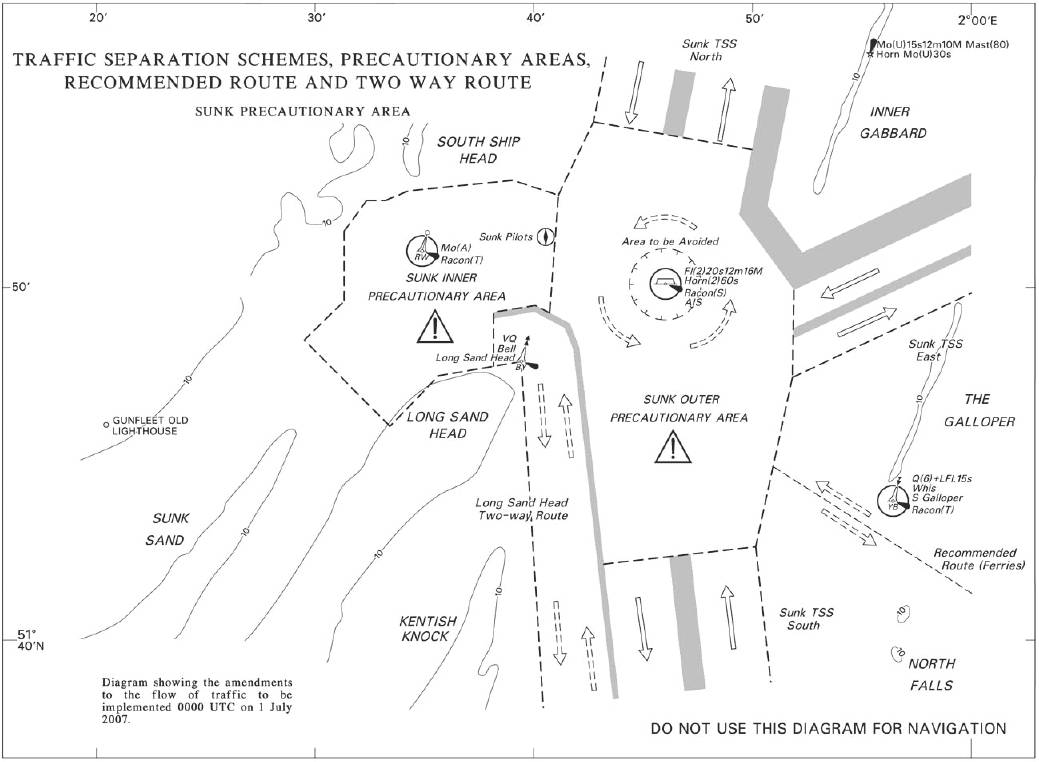
\includegraphics[scale=0.3]{figs/COLREGS_10_TSS_1.png}
                \caption{Traffic Separation Scheme Example \cite{yachtcluTSS}}
                \label{fig:COLREGS_10_TSS_1}
            \end{figure}
            
            Possible implementation: Change guidance according to \acp{TSS}.
            
        \item Rule 11 - Rules 11-18 must be followed when vessels encounters happen.
        \item Rule 13 - Overtaking (PARAPHRASED):
        
            \begin{itemize}
                \item "Any vessel overtaking any other shall \underline{keep out of the way} of the vessel being overtaken."
                \item "A vessel shall be deemed to be overtaking when coming up with another vessel from a direction more than 22.5 degrees abaft her beam, that is, in such a position with reference to the vessel she is overtaking, that at night she would be able to see only the sternlight of that vessel but neither of her sidelights."(c).
                \item "When a vessel is in any doubt as to whether she is overtaking another, she shall assume that this is the case and act accordingly."
                \item "Any subsequent alteration of the bearing between the two vessels shall not make the overtaking vessel a crossing vessel within the meaning of these Rules or relieve her of the duty of keeping clear of the overtaken vessel until she is finally past and clear."
            \end{itemize}
            
            Possible implementation: Overtaking action with degrees constraint. Detect if the \ac{USV} is being overtaken and then apply constraints to the guidance system to avoid actions that can generate dangerous situations.
            
            An example of this scenario is presented in Figure \ref{fig:COLREGS_Rule13}:
            \begin{figure}[H]
                \centering
                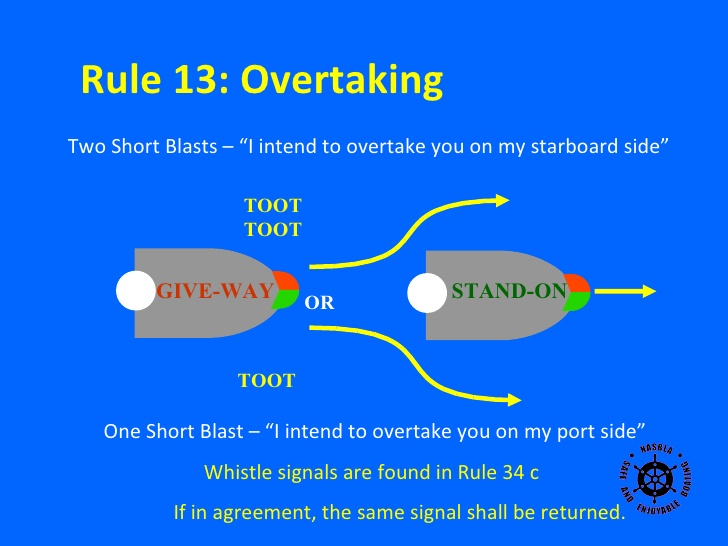
\includegraphics[scale=0.45]{figs/COLREGS_Rule13.jpg}
                \caption{Overtaking Situation \cite{nasbla2009}}
                \label{fig:COLREGS_Rule13}
            \end{figure}
            
        \item Rule 14 - Head-On (PARAPHRASED):
        
            \begin{itemize}
                \item "When two power-driven vessels are meeting on \underline{reciprocal or nearly reciprocal} courses so as to involve risk of collision each shall alter her course to starboard so that each shall pass on the port side of the other."
            \end{itemize}
            
            Possible implementation: Head-on collision avoidance action.
            
            An example of this scenario is presented in Figure \ref{fig:COLREGS_Rule14}:
            \begin{figure}[H]
                \centering
                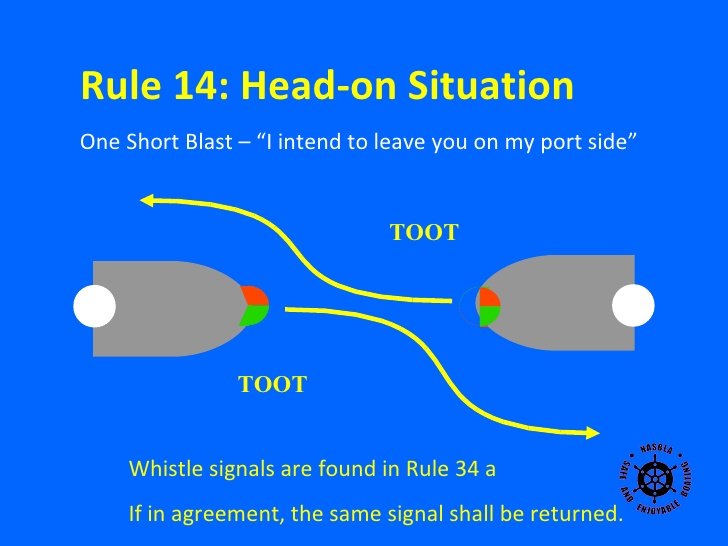
\includegraphics[scale=0.45]{figs/COLREGS_Rule14.jpg}
                \caption{Head-on Situation \cite{nasbla2009}}
                \label{fig:COLREGS_Rule14}
            \end{figure}
            
       \item Rule 15 - Crossing (PARAPHRASED):
        
            \begin{itemize}
                \item "When two power-driven vessels are crossing \underline{so as to involve risk of collision}, the vessel which has the other on her own starboard side shall keep out of the way and shall, if the circumstances of the case admit, avoid crossing ahead of the other vessel."
            \end{itemize}
            
            Possible implementation: Crossing collision avoidance action.
            
            An example of this scenario is presented in Figure \ref{fig:COLREGS_Rule15}\cite{nasbla2009}:
            \begin{figure}[H]
                \centering
                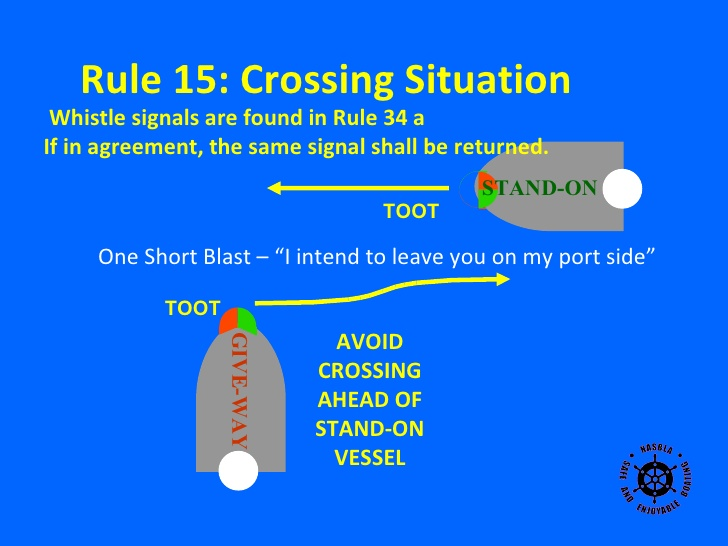
\includegraphics[scale=0.45]{figs/COLREGS_Rule15.jpg}
                \caption{Crossing Situation \cite{nasbla2009}}
                \label{fig:COLREGS_Rule15}
            \end{figure}
            
        \item Rule 16 - Action by give-way vessel (PARAPHRASED):
        
            \begin{itemize}
                \item "Every vessel which is directed to keep out of the way of another vessel shall, so far as possible, take \underline{early and substantial} action to keep \underline{well clear}."
            \end{itemize}
        
        \item Rule 17 - Action by stand-on vessel (PARAPHRASED):
        
            \begin{itemize}
                \item "Where one of two vessels is to keep out of the way the other shall keep her course and speed"
                \item "The latter vessel may however take action to avoid collision by her manoeuvre alone, as soon as it \underline{becomes apparent to her} that the vessel required to keep out of the way is not taking appropriate action in compliance with these Rules."
                \item "When, from any cause, the vessel required to keep her course and speed finds herself so close that collision cannot be avoided by the action of the give-way vessel alone, she shall take such action as will best aid to avoid collision."
            \end{itemize}
            
        \item Rule 18 - Responsibilities between vessels:
        
            There is a hierarchy of responsibilities. More powerful and robust vessels are more responsible by maneuver than less powerful or less robust. Power-driven vessel underway shall keep out of the way of a vessel not under command, a vessel restricted in its ability to maneuver, a vessel engaged in fishing, and a sailing vessel. Sailing vessel underway shall keep out of the way of a vessel not under command, a vessel restricted in its ability to maneuver, and a vessel engaged in fishing. A vessel engaged in fishing underway shall keep out of the way of a vessel not under command, and a vessel restricted in its ability to maneuver.
            
            Possible implementation: The \ac{USV} system could be capable of detecting and identify other types of vessel, this could lead to a change of action.
            
        \item Rule 23 - Power-driven vessels underway (PARAPHRASED):
        
            \begin{itemize}
                \item "A power-driven vessel underway shall exhibit:"
                \begin{itemize}
                    \item "a masthead light forward;"
                    \item "sidelights;"
                    \item "a sternlight."
                \end{itemize}   
                \item "A power-driven vessel of less than 12 metres in length may in lieu of the lights prescribed in paragraph (a) of this Rule exhibit an all-round white light and sidelights;"
                \item "A power-driven vessel of less than 7 metres in length whose maximum speed does not exceed 7 knots may exhibit an all-round white light and shall, if practicable, also exhibit sidelights;"
            \end{itemize}
            
            Possible implementation: real boat requirements for tests.
            
        \item Rule 27 - Vessels not under command or restricted in their ability to maneuver (PARAPHRASED):
        
        \begin{itemize}

            \item "A vessel not under command shall exhibit:" 
                \begin{itemize}
            
                    \item "two all-round red lights in a vertical line where they can best be seen;" 
                    \item "two balls or similar shapes in a vertical line where they can best be seen;"
                    \item "when making way through the water, in addition to the lights prescribed in this paragraph, sidelights and a sternlight."
            
                \end{itemize}
            \item "A vessel restricted in her ability to manoeuvre, except a vessel engaged in mine clearance operations, shall exhibit:"
                \begin{itemize}
        
                \item "three all-round lights in a vertical line where they can best be seen. The highest and lowest of these lights shall be red and the middle light shall be white;"
                \item "three shapes in a vertical line where they can best be seen. The highest and lowest of these shapes shall be balls and the middle one a diamond;"
        
            \end{itemize}
        \end{itemize}
        
        \item Rule 33 - Equipment for sound signals: A vessel of less than 12 meters in length shall be provided with some means of making an efficient sound signal.

    \end{itemize}
    
    The highlighted rules above will be used in the research proposal of this document. 
    From them we can have a glance of the non-objectiveness or ambiguity of some terms used for rules definition such as proper look-out", "safe speed", "ample time", "large enough", and others. Some rules are related to possible or mandatory features required for a \ac{USV} system, such as 9, 10, 13, 14, 15, 16, 17, and 18. Also, other rules are related to structural requirements for \ac{USV}s in real-world trials, such as 23, and 33.
    
    \ac{COLREGS} rules were not defined considering autonomous systems such as \ac{USV}s. They were written to be interpreted by well-experienced sailors and imply usage of their experience and common sense. There are gaps to be filled and subjective or ambiguous definitions to be addressed, making the development of a \ac{COLREGS}-compliant \ac{USV} guidance system challenging.
    % VJ: reorganizar

    \subsection{Surface Vehicle Modeling}
    \subsection{Configuration Space}
    \subsection{Planning Algorithms}
\chapter{Literature Review \label{chap:3_LiteratureReview}}

    % I could consult Candeloro2017Voronoi Literature Review

    In this chapter, we discuss the related studies, identifying their main contributions related to the development of global and local guidance systems for \ac{USV}. 
    The focus of this chapter is to highlight commonly used guidance methods, and explain in detail \ac{COLREGS}-compliant collision avoidance techniques presented in the literature.
    
    \section{Literature Review}

    %%%%%%%%%%%%%%%%%%%%%%%%%%%%%%%%%%%%%%%%%%%% Larson2006Autonomous
    \subsection{Larson 2006 Autonomous}
    Larson \etal~\cite{Larson2006Autonomous} explore the usage of A* in combination with \ac{VO}\footnote{In robotics and motion planning, a velocity obstacle, commonly abbreviated VO, is the set of all velocities of a robot that will result in a collision with another robot at some moment in time, assuming that the other robot maintains its current velocity.} \cite{Fiorini1998Motion} as path planner for global guidance. A* is used to avoid stationary obstacles, and \ac{VO} is used to avoid dynamic obstacles such as other vessels. The navigation is based on waypoints, and the global guidance system is responsible for the continuous modification of existing waypoints route to plan around obstacles detected with long-range sensors, such as \ac{AIS}, \ac{ARPA} contacts, and nautical charts. The \ac{AIS} system receives position, speed, and course data broadcasts from other marine vessels with compatible systems. The \ac{ARPA} system is capable of creating tracks using radar contacts and can calculate the tracked object's course, speed, and \ac{CPA}\footnote{Closest Point of Approach refers to the positions at which two dynamically moving objects reach their closest possible distance. \ac{CPA} is an important calculation for collision avoidance.}, thereby knowing whether there is a risk of collision with other ships or moving obstacles. Nautical charts can provide information about water depth, land heights, coastline, safe ways, navigational hazards, tides, currents, and human-made structures such as harbors, buildings, and bridges. Nautical charts are used as basic information for running A* and definition of waypoints. \ac{AIS} and \ac{ARPA} are used as basic information for running \ac{VO} and definition of waypoints.
    
    For local guidance, Larson \etal~\cite{Larson2006Autonomous} combines the information provided by a perception system for the generation of a local world-model. The perception system for near-field obstacles detection is composed of \ac{MWR}, Stereo Vision, Monocular Camera, and \ac{LADAR}. When an obstacle is detected, the new trajectory is defined based on the local world-model and a behavior-based approach. There are three behaviors: keep the last planned path, collision avoidance path, and free-space path. The decision is made through a voting system where the collision avoidance behavior vote is two times heavier than the others (\ie 2:1:1) and generates paths in an arc format, as shown in Figure \ref{fig:Larson2006Autonomous_Arcs}. Figure \ref{fig:Larson2006Automated_Summary} present a summary of Larson \etal~ work, the green path is the initial trajectory determined through A*, the blue path is the corrected trajectory for the avoidance of dynamic obstacles detected, and the red dots show the predicted trajectory of each obstacle using the \ac{VO} method.
    
    \begin{figure*}[t!]
    \centering
    
        \begin{subfigure}[t]{0.35\textwidth}
            \centering
            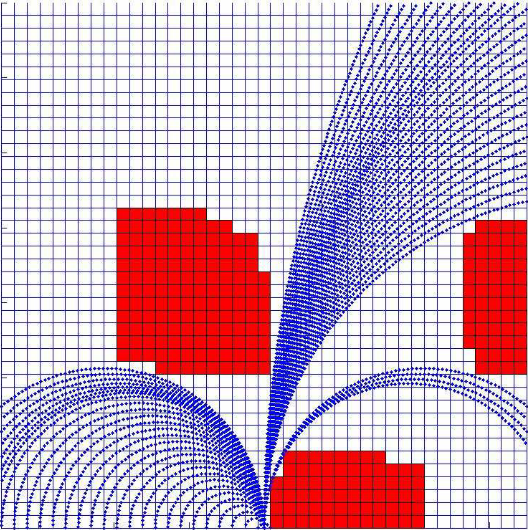
\includegraphics[width=0.75\textwidth]{figs/Chap3/Larson2006Autonomous_Arcs.png}
            \subcaption{Arc Path}
            \label{fig:Larson2006Autonomous_Arcs}
        \end{subfigure}%
        ~ 
        \begin{subfigure}[t]{0.6\textwidth}
            \centering
            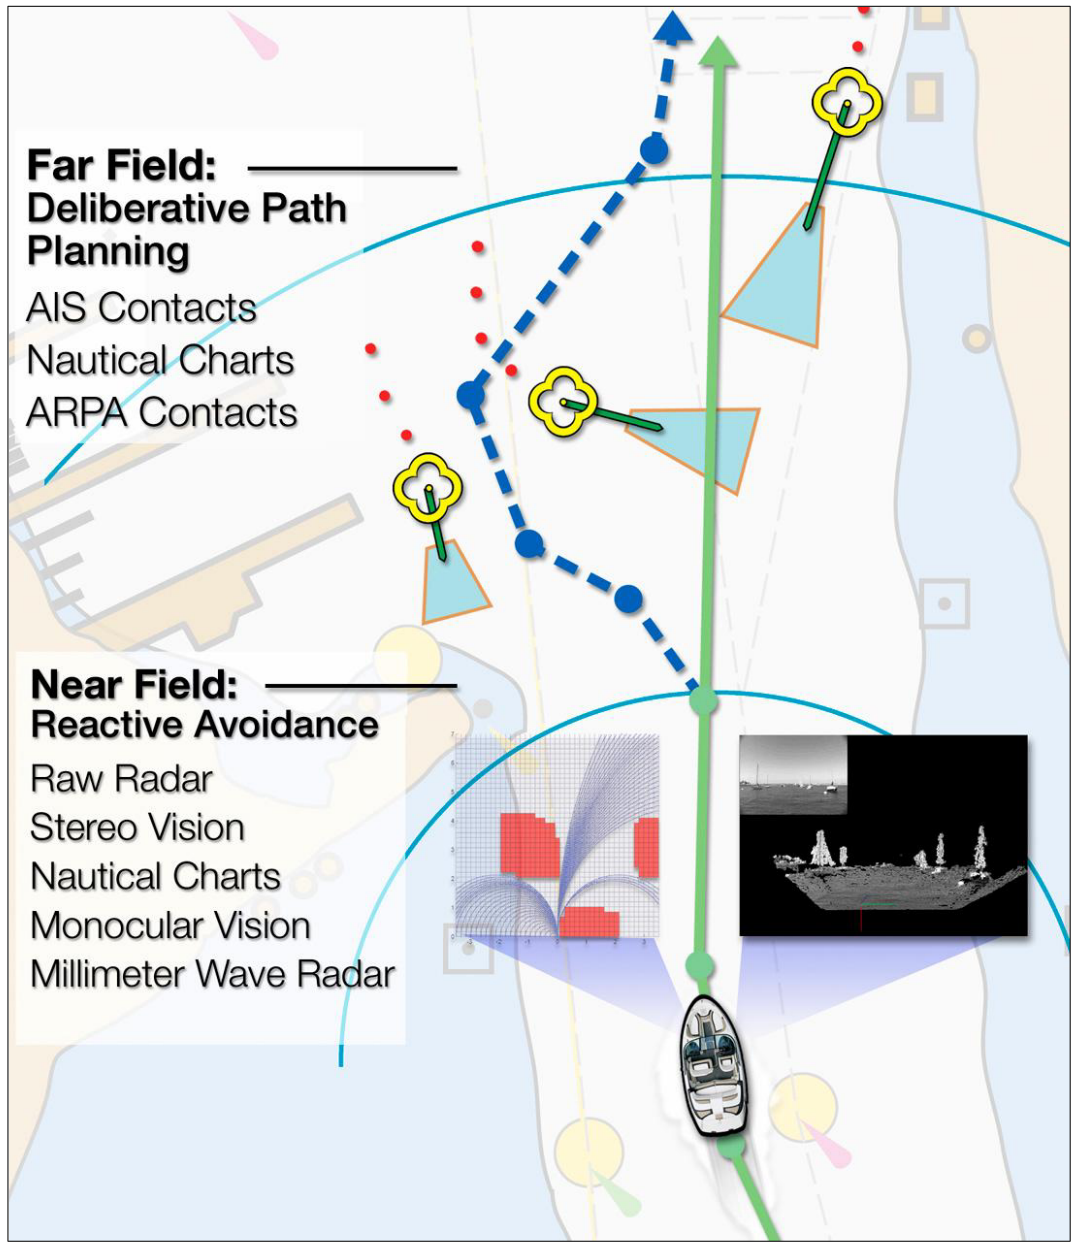
\includegraphics[width=\textwidth]{figs/Chap3/Larson2006Automated_Summary.png}
            \subcaption{Global Guidance Trajectories}
            \label{fig:Larson2006Automated_Summary}
        \end{subfigure}
        
    \caption{Guidance System Trajectories \cite{Larson2006Autonomous}}
    \end{figure*}
    %%%%%%%%%%%%%%%%%%%%%%%%%%%%%%%%%%%%%%%%%%%%
    
    %%%%%%%%%%%%%%%%%%%%%%%%%%%%%%%%%%%%%%%%%%%% Agrawal2015COLREGS
    \subsection{Agrawal 2015 COLREGS}
    Agrawal \etal~\cite{Agrawal2015COLREGS} present an \ac{USV} \ac{COLREGS}-compliant path planning strategy to follow another vessel in dynamic environments. Their solution is capable of predicting the target vessel motion, and then plan the route towards the target vessel while respecting the \ac{COLREGS}. 
    
    For collision avoidance, the system identifies \ac{COLREGS} conditions that apply to the current situation, in a specific time, considering nearby vessels and for each vessel is calculated the \ac{CPA}. If the \ac{CPA} is smaller than a threshold distance but not critical, the path is re-planned using A* with restriction in the search space for compliance to the \ac{COLREGS}.  When a critical distance is detected, the system re-plan using A* without restrictions in the search space. 
    
    For global guidance, the path is chosen based on the predicted motion for the target vessel using Monte-Carlo sampling of dynamically feasible and collision-free paths with fuzzy weights. The prediction is continuously optimized for a particular target by learning the necessary parameters for a 3-degree-of-freedom model of the vessel and its maneuvering behavior from its path history without any prior knowledge.
    
    For validation, they performed field tests on Panther Hollow Lake in Pittsburgh, PA, USA. They used 1.8m-long kayaks fitted with underwater-scooter motors on either side for propulsion, batteries, computers, compass, GPS, LIDAR scanners for obstacle detection, and RF receivers for manual control. The target-vessel was manually controlled at a speed of 1.7 m/s, and the presented test scenarios contain one civilian vessel that must be avoided. They successfully tested head-on and overtaking situations.
    %%%%%%%%%%%%%%%%%%%%%%%%%%%%%%%%%%%%%%%%%%%% 
    
    %%%%%%%%%%%%%%%%%%%%%%%%%%%%%%%%%%%%%%%%%%%%  Naeem2012COLREGS
    \subsection{Naeem 2012 COLREGS}
    For global guidance, Naeem \etal~\cite{Naeem2012COLREGS} use an A*-based algorithm, named \ac{DPSS}. 
    This method is based on a goal direction vector capable of reducing the search time by up to 50\%\cite{Yang2010Efficient}. The \ac{DPSS} algorithm produces waypoints around obstacles that form a smoother path with less sharp turns than A*. For local guidance, they use waypoint trajectory definition by \ac{LOS} \cite{Healey1993Multivariable}. Regarding \ac{COLREGS}-compliant collision avoidance, they present a manual biasing scheme consisting of always sailing towards the \ac{USV} starboard side to avoid collision situations with detected objects. They argue that avoiding obstacles always heading towards the starboard side makes the system compliant to the \ac{COLREGS}. However, this is not a good strategy since this action may lead to violation of other \ac{COLREGS} rules such as rule 10 that impose that navigation must respect \acf{TSS}.
    For dynamic obstacle detection, it is suggested the use of \ac{LIDAR} and cameras, and for the navigation system, they suggest the use of \ac{GPS}. The guidance system is evaluated through software simulation, where the control system uses a simple \ac{PID} for autopiloting.
        
    For collision avoidance, Naeem \etal~assume a \ac{COR} around each detected obstacle (shown in Figure \ref{fig:Naeem2012COLREGS_Trajectories_StaticObstacles}). For navigation Naeem \etal~assume a \ac{COA} around each waypoint. After the \ac{USV} enters the \ac{COA} the mission planner selects the next waypoint. Every time the distance between the \ac{USV} and an obstacle is less or equal than the \ac{COR}, the local guidance system becomes responsible for path plan generation. The system addresses collision avoidance for both dynamic and stationary obstacles. Figure \ref{fig:Naeem2012COLREGS_Trajectories_StaticObstacles} shows the generated trajectories using \ac{LOS} and \ac{DPSS} for avoid collision with static obstacles. Moreover, Figure \ref{fig:Naeem2012COLREGS_Trajectories_DynamicObstacles} shows a \ac{COLREGS}-compliant collision avoidance scenario, with dynamic obstacles.
    
    \begin{figure}[H]
    \centering
    
        \begin{subfigure}[b]{0.5\textwidth}
            \centering
            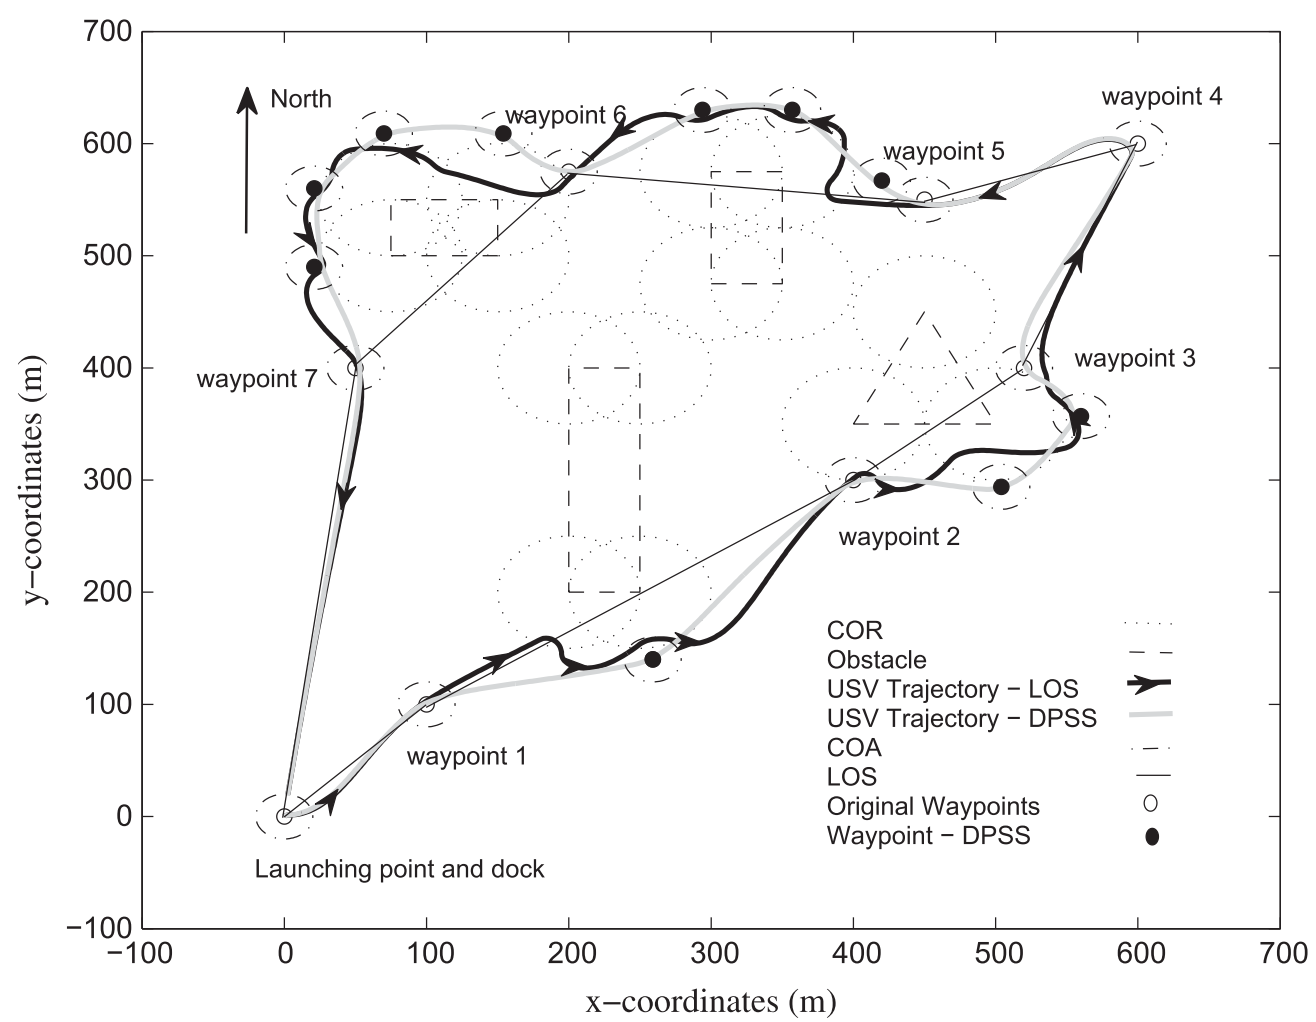
\includegraphics[width=\textwidth]{figs/Chap3/Naeem2012COLREGS_Trajectories_StaticObstacles.png}
            \caption{Static Obstacles}
            \label{fig:Naeem2012COLREGS_Trajectories_StaticObstacles}
        \end{subfigure}
        \begin{subfigure}[b]{0.4\textwidth}
            \centering
            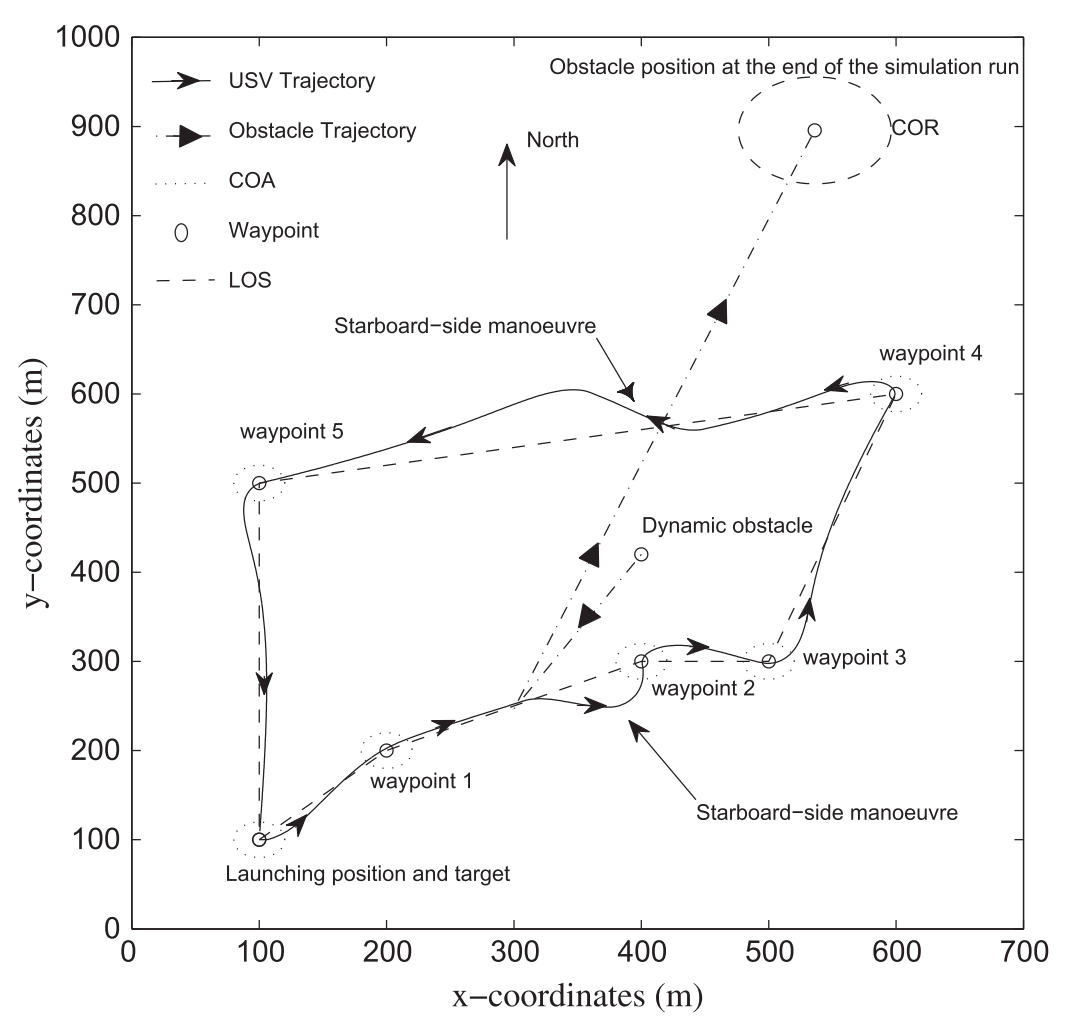
\includegraphics[width=\textwidth]{figs/Chap3/Naeem2012COLREGS_Trajectories_DynamicObstacles.png}
            \caption{Dynamic Obstacles}
            \label{fig:Naeem2012COLREGS_Trajectories_DynamicObstacles}
        \end{subfigure}
    
    \caption{Obstacles Avoidance Simulations \cite{Naeem2012COLREGS}}
    \label{fig:Naeem2012COLREGS_Trajectories}
    \end{figure}
    %VJ Explique a figura e o que é cada coisa na legenda e no texto.
    %%%%%%%%%%%%%%%%%%%%%%%%%%%%%%%%%%%%%%%%%%%% 
    
    %%%%%%%%%%%%%%%%%%%%%%%%%%%%%%%%%%%%%%%%%%%%  Campbell2013Automatic
    \subsection{Campbell 2013 Automatic}
    For obstacle avoidance, Campbell \etal~\cite{Campbell2013Automatic} present a system composed of a unit to predict the next position of detected obstacles. They use the \ac{CPA} method, assuming that detected obstacles will keep proceeding in their current velocities, this method finds the closest distance between encountering vessels at some time in the future. Moreover, a sampling interval is determined for updating the calculated distance. If the closest predicted distance is less than the acceptable range, the module advises a change in direction when an approaching threat is confirmed. The perception system is composed of a Microsoft HD video camera for object detection and identification and an Acuity laser range finder, so the basic information necessary for obstacle detection is extracted through the analysis of the data captured by the perception system. Moreover, the trajectory of the obstacles are predicted using Equations~\ref{eq:X} and \ref{eq:Y},
    \begin{equation}
    \label{eq:X}
    X = X_p + \int V cos(\psi)dt
    \end{equation}
    \begin{equation}
    \label{eq:Y}
    Y = Y_p + \int V sin(\psi)dt,
    \end{equation}
    where the pair \textit{X} and \textit{Y} is the predicted position, the pair $X_p$ and $X_y$ is the current position, and $\psi$ is current heading angle
    
    For global guidance, the system uses A*, and for local guidance, they use a modification of A*, named \ac{R-RA*}. The focus of this work is on describing the local guidance system. The \ac{R-RA*} method consists of having the path generated by A* as the base, and then perform iterative changes in the path to avoid collisions applying constraints to the search space. Path changes are performed in a local scope. The constraining is done on each iteration through the evaluation of the nodes in the search space and the addition of unwanted nodes to the A* closed list. That is, positions that violate the \ac{COLREGS} are marked as belonging to the closed list. This way, A* will not consider those nodes. The world is locally represented using a grid. A core assumption of the method is that \ac{USV}s can always determine other vessels' heading and velocity. The system uses this information for the calculation of the \ac{CPA}. The navigation system is composed by GPS and gyrocompass. Every time the distance between the \ac{USV} and the \ac{CPA} is shorter than the minimum acceptable distance, the local guidance system, with \ac{R-RA*} is activated. For system evaluation, they performed virtual simulations using the Virtual Sailor Simulator\footnote{Papini I. Virtual Sailor Software. SimSquared Ltd. Ship Simulator Shareware, 1999–2017. http://www.hangsim.com/virtual-sailor/}.
    %%%%%%%%%%%%%%%%%%%%%%%%%%%%%%%%%%%%%%%%%%%% 
    
    %%%%%%%%%%%%%%%%%%%%%%%%%%%%%%%%%%%%%%%%%%%%  Naus2013Idea
    \subsection{Nauss 2013 Idea}
    In Naus \etal~\cite{Naus2013Idea} the global guidance system uses A* for path planning. 
    Static data about the environment (\ie~topography, coastline, and safe way) is extracted from electronic navigational charts, and dynamic data (\ie~position of other ships) is extracted from \ac{DGPS}\footnote{Differential Global Positioning Systems (DGPS) are enhancements to the Global Positioning System (GPS) which provide improved location accuracy, in the range of operations of each system, from the 15-meter nominal GPS accuracy to about 10 cm in case of the best implementations.}, \ac{AIS}, and \ac{ARPA} sensors. This information is used to generate a map representation of the world and the sequential execution of the A* to determine the path to be followed by the \ac{USV}. This paper does not address the problem of collision avoidance for local guidance.
    %%%%%%%%%%%%%%%%%%%%%%%%%%%%%%%%%%%%%%%%%%%% 
    
    %%%%%%%%%%%%%%%%%%%%%%%%%%%%%%%%%%%%%%%%%%%%  Annamalai2013Comparison
    \subsection{Annamalai 2013 Comparison}
    Annamali \etal~\cite{Annamalai2013Comparison} focus on developing a control system but discuss the usage of a waypoint \ac{LOS} scheme \cite{Healey1993Multivariable} for global guidance. The \ac{USV} tries to go straight ahead from its current position until the next waypoint. For waypoint, following the control system was composed of a \ac{MPC} autopilot. In order to decide whether a waypoint has been reached or not, the guidance system considers a \ac{COA} around each waypoint. The suggested \ac{COA} radius is equal to the length of the vessel. The navigation system is equipped with \ac{GPS} for the determination of the current localization. For the determination of the current heading of the \ac{USV}, they combine the information provided by three electronic compasses (TCM2, HMR3000, and KVH-C100). For evaluation, the system was tested in simulated scenarios. This paper does not address the problem of local guidance.
    %%%%%%%%%%%%%%%%%%%%%%%%%%%%%%%%%%%%%%%%%%%% 
    
    %%%%%%%%%%%%%%%%%%%%%%%%%%%%%%%%%%%%%%%%%%%%  Lee2004Fuzzy
    \subsection{Lee 2004 Fuzy}
    Lee \etal~\cite{Lee2004Fuzzy} propose the use of \ac{VFF}\cite{Borenstein1989Real} for \ac{USV} \ac{COLREGS}-compliant collision avoidance. They present the \ac{MVFF} method, a modification of the traditional \ac{VFF} algorithm based on fuzzy logic. The focus is on the determination of the desired \ac{USV} heading angle $\Psi_d$ components. The geometric terms proposed consist of track-keep $\Psi_{tk}$, and collision avoidance angles $\Psi_{ca}$. 
    % VJ: usage vs use, no difference: less characters to type... #ficadica
    % VJ: mathematical components proposed? Acho melhor reescrever isso.
    The \ac{USV} route is defined by waypoints, where the path between consecutive waypoints is considered a straight line. However, movements that distance the \ac{USV} from the desired path may happen, for example, when a collision avoidance movement is required. Therefore, \ac{USV} motion strategy considers a combination of go towards the goal/next waypoint behavior and keep on tracking behavior. The heading angle mainly defines the motion of the \ac{USV}. Lee \etal~define the following formula for the desired heading angle:
    % VJ: eu resscrevi um pouco do parágrafo pois estava redundante. Explico: waypoints são pontos que devem ser seguidos. Desnecessário escrever isso.
    % VJ: Você está esquecendo de colocar virǵulas entre conectivos repetidamente. Cuidado redobrado ao iniciar frases.
    % VJ: Não é apenas desejável a combinação. Sem ela o robô pode não atingir o objetivo. Por isso eles combinaram os ângulos.
    % VJ Acho que os parágrafos acima e abaixo estão confusos e podem ser melhorados. Acima reescrever "The heading angle mainly defines the motion of the \ac{USV}". O texto do parágrafo abaixo pode ser combinado com a reescrita acima
    \begin{equation}
    \Psi_d = \Psi_{tk} + \Psi_{ca}
    \end{equation}
    % VJ: Dica sobre fórmula. Pense sempre assim: o símbolo tal representa, é, xpto, enquanto o símbolo bla é, representa, depicts xpto. Ou seja Psi-tk é o ângulo entre ..., whule psi_ca é bla.  
    The $\Psi_{tk}$ angle is related to a combination of the virtual forces that attract the \ac{USV}, respecting a proportion, to the desired track, and towards the goal. The $\Psi_{ca}$ angle is defined using fuzzy logic after the detection of obstacle direction, orientation, distance, relative velocity, and position relative to the \ac{USV}. Each detected value is translated into a weight for fuzzy logic decision. 
    
    Figure \ref{fig:Lee2004Fuzzy_tkAngle} illustrates a scenario where the \ac{USV} is relatively far from the desired track and must go to the Waypoint 2, $\vec{e}_a$  and $\vec{e}_p$ are the virtual forces related to the $\Psi_{ca}$ angle. Figure \ref{fig:Lee2004Fuzzy_caAngle} shows a similar scenario, but the \ac{USV} must avoid the obstacle present. The collision avoidance angle guides the avoidance.
    \begin{figure}[H]
    \centering
        \begin{subfigure}[b]{0.5\textwidth}
            \centering
            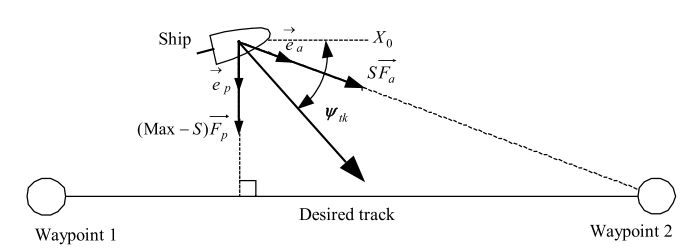
\includegraphics[width=\textwidth]{figs/Chap3/Lee2004Fuzzy_tkAngle.png}
            \caption{Track-Keep Angle}
            \label{fig:Lee2004Fuzzy_tkAngle}
        \end{subfigure}
        \begin{subfigure}[b]{0.4\textwidth}
            \centering
            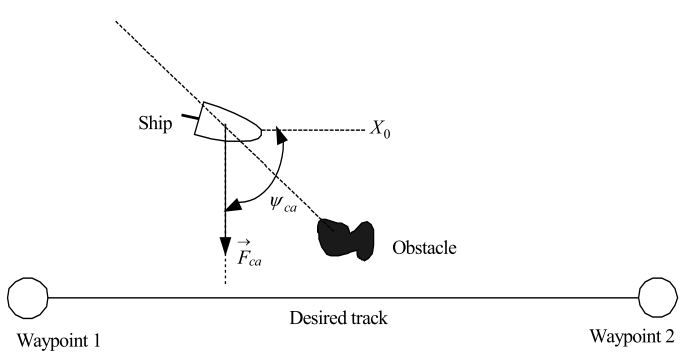
\includegraphics[width=\textwidth]{figs/Chap3/Lee2004Fuzzy_caAngle.png}
            \caption{Collision Avoidance Angle}
            \label{fig:Lee2004Fuzzy_caAngle}
        \end{subfigure}
    
    \caption{Vectors for angles determination \cite{Lee2004Fuzzy}}
    \label{fig:Lee2004Fuzzy_Angles}
    \end{figure}
    
    For simplicity, Lee \etal~\cite{Lee2004Fuzzy} assumed that the \ac{USV} is capable of only turn right. Simulation tests demonstrate that the presented method is applicable for implementation of \ac{COLREGS} rules 13, 14, 15, and 17 as presented in Figure \ref{fig:Lee2004Fuzzy_COLREGS_13_14_15_17}. 
    \begin{figure}[H]
    \centering
    
        \begin{subfigure}[b]{0.5\textwidth}
            \centering
            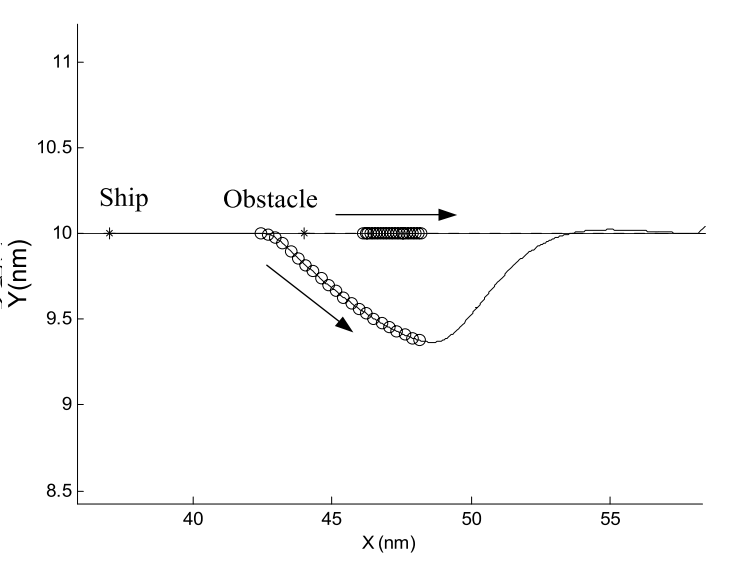
\includegraphics[width=\textwidth]{figs/Chap3/Lee2004Fuzzy_COLREGS13.png}
            \caption{\ac{COLREGS} rule 13}
            \label{fig:Lee2004Fuzzy_COLREGS13}
        \end{subfigure}
        \begin{subfigure}[b]{0.45\textwidth}
            \centering
            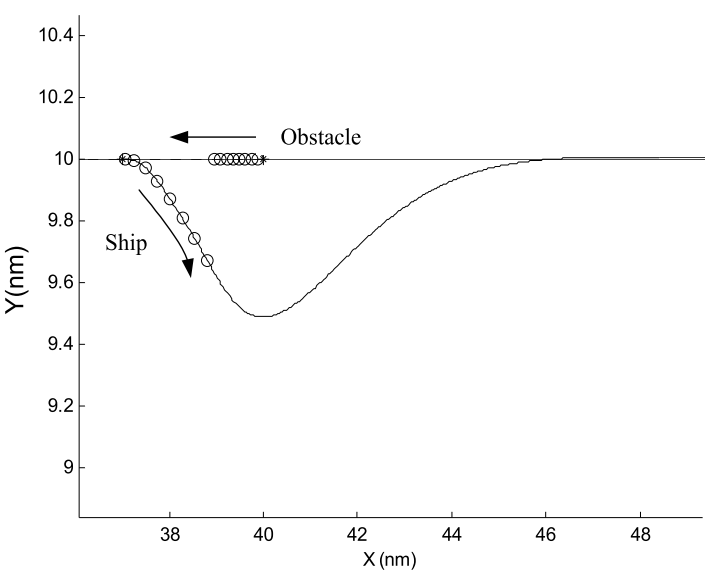
\includegraphics[width=\textwidth]{figs/Chap3/Lee2004Fuzzy_COLREGS14.png}
            \caption{\ac{COLREGS} rule 14}
            \label{fig:Lee2004Fuzzy_COLREGS14}
        \end{subfigure}
        
        \begin{subfigure}[b]{0.5\textwidth}
            \centering
            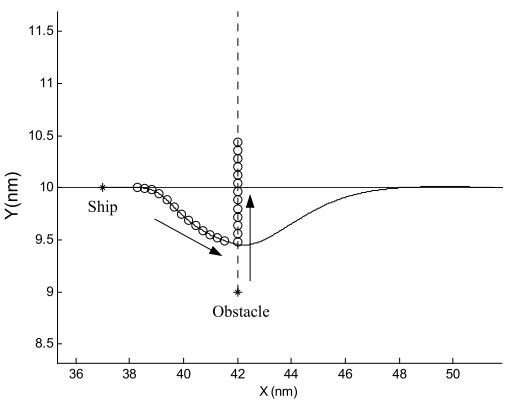
\includegraphics[width=\textwidth]{figs/Chap3/Lee2004Fuzzy_COLREGS15a.png}
            \caption{\ac{COLREGS} rule 15}
            \label{fig:Lee2004Fuzzy_COLREGS15}
        \end{subfigure}
        \begin{subfigure}[b]{0.45\textwidth}
            \centering
            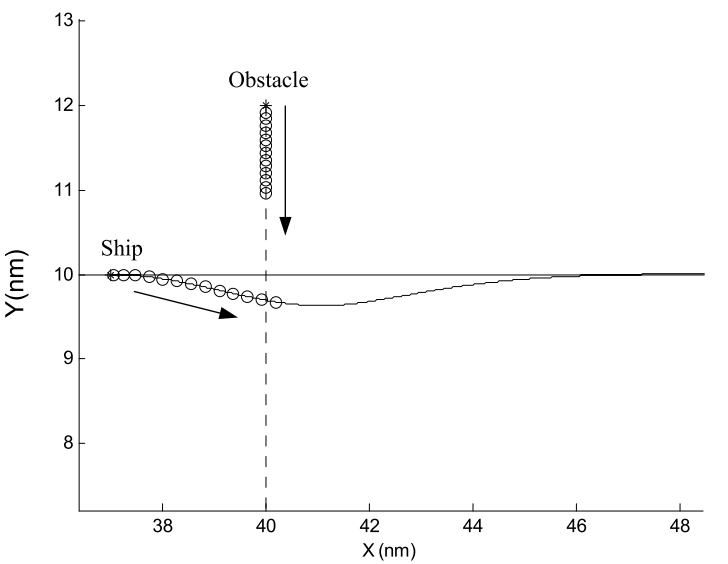
\includegraphics[width=\textwidth]{figs/Chap3/Lee2004Fuzzy_COLREGS18.png}
            \caption{\ac{COLREGS} rule 17}
            \label{fig:Lee2004Fuzzy_COLREGS18}
        \end{subfigure}
    
    \caption{Simulated tests \cite{Lee2004Fuzzy}}
    \label{fig:Lee2004Fuzzy_COLREGS_13_14_15_17}
    \end{figure}
    %%%%%%%%%%%%%%%%%%%%%%%%%%%%%%%%%%%%%%%%%%%%
    
    %%%%%%%%%%%%%%%%%%%%%%%%%%%%%%%%%%%%%%%%%%%% Kuwata2014Safe
    \subsection{Kuwata 2014 Safe}
    Kuwata \etal~\cite{Kuwata2014Safe} present a \ac{COLREGS}-compliant local guidance system based on \ac{VO} capable of addressing static and dynamic obstacles. Detection of dangerous situations is done through analyses of the \ac{CPA} and the geometric constraints presented in Figure~\ref{fig:Kuwata2014Safe_GeometricConstraints}, but the specific angles were not clearly defined. Environment information about static and dynamic obstacles are captured through a perception system composed of a radar, stereo cameras, and \ac{LIDAR}. On real-world tests, the \ac{USV} state is estimated by an onboard inertial navigation system. They discuss that \ac{VO} is an intuitive way to implement \ac{COLREGS} since \ac{VO} works on applying constraints to the \ac{USV} possible velocity space. Therefore, apply \ac{COLREGS} through \ac{VO} consists of applying some more constraints to the possible velocity space. They present the constraints used to implement \ac{COLREGS} rules 13 (overtaking), 14 (head-on), and 15 (crossing). For system evaluation, they executed real-world trials, and the \ac{USV} was exposed to around 30 scenarios with single and multiple vessel encounters. The \ac{USV} successfully acted on 24 maneuvers avoiding collision and did not respond safely to only one situation due to a vision sensor problem. They do not address global guidance system development.
    
    \begin{figure}[H]
        \centering
        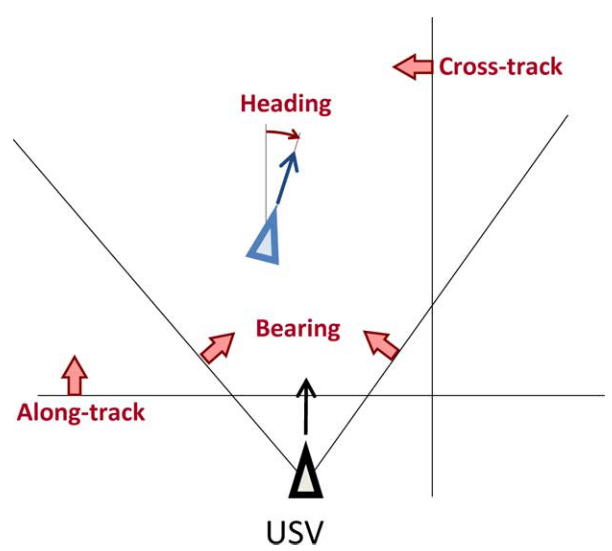
\includegraphics[scale=0.4]{figs/Chap3/Kuwata2014Safe_GeometricConstraints.png}
        \caption{Angle Analysis for Identification of Dangerous Situations \cite{Kuwata2014Safe}}
        \label{fig:Kuwata2014Safe_GeometricConstraints}
    \end{figure}
    
    %%%%%%%%%%%%%%%%%%%%%%%%%%%%%%%%%%%%%%%%%%%%
    
    %%%%%%%%%%%%%%%%%%%%%%%%%%%%%%%%%%%%%%%%%%%% Benjamin2004COLREGS
    For collision avoidance on local guidance, Benjamin \etal~\cite{Benjamin2004COLREGS} explore the use of a technique named Behavior-based Control and Multi-objective Action Selection. Different behaviors are defined corresponding to each possible situation, such as obstacle avoidance or keep the current mission. Each behavior defines objective functions that rates all possible actions concerning the corresponding \ac{COLREGS} rule. The decision space for vehicle action is defined based on variables such as course, speed, and intended-time. Tests are performed with four real kayaks. The navigation system is capable of determining its position from \ac{GPS}. Also, the \ac{USV} broadcasts their positions to each other. There is no specific detection system, after receiving position information, the \ac{USV} assumes that the \ac{GPS} information received corresponds to another \ac{USV} with which it must avoid collision.
    %%%%%%%%%%%%%%%%%%%%%%%%%%%%%%%%%%%%%%%%%%%%
    
    %%%%%%%%%%%%%%%%%%%%%%%%%%%%%%%%%%%%%%%%%%%%  Zhuang2011Motion
    \subsection{Zhuang 2011 Motion}
    In Zhuang \etal~\cite{Zhuang2011Motion}, they declare the usage of an evolutionary path planner~\cite{Russel2003AI_GA} for global guidance but do not specify which one and do not define clearly if the system is capable of dealing with static and dynamic obstacles. For local guidance, they used the \ac{VO} method \cite{Fiorini1998Motion}. Dangerous situations can happen in different forms, head-on encounter, crossing, overtaking. For the identification of different situations, the system is based on geometric constraints with limits defined by angles related to the \ac{USV} heading. As shown in figure \ref{fig:Zhuang2011Motion_Sectors}, the \ac{USV} heading is the 0° angle, 15° from the \ac{USV} angle defines the head-on encounter sector. A crossing is defined 135° from \ac{USV} heading. The system is evaluated through software simulation, and the results presented show that the local guidance system is compliant to \ac{COLREGS} rules 14 and 15.
    
    \begin{figure}[H]
        \centering
        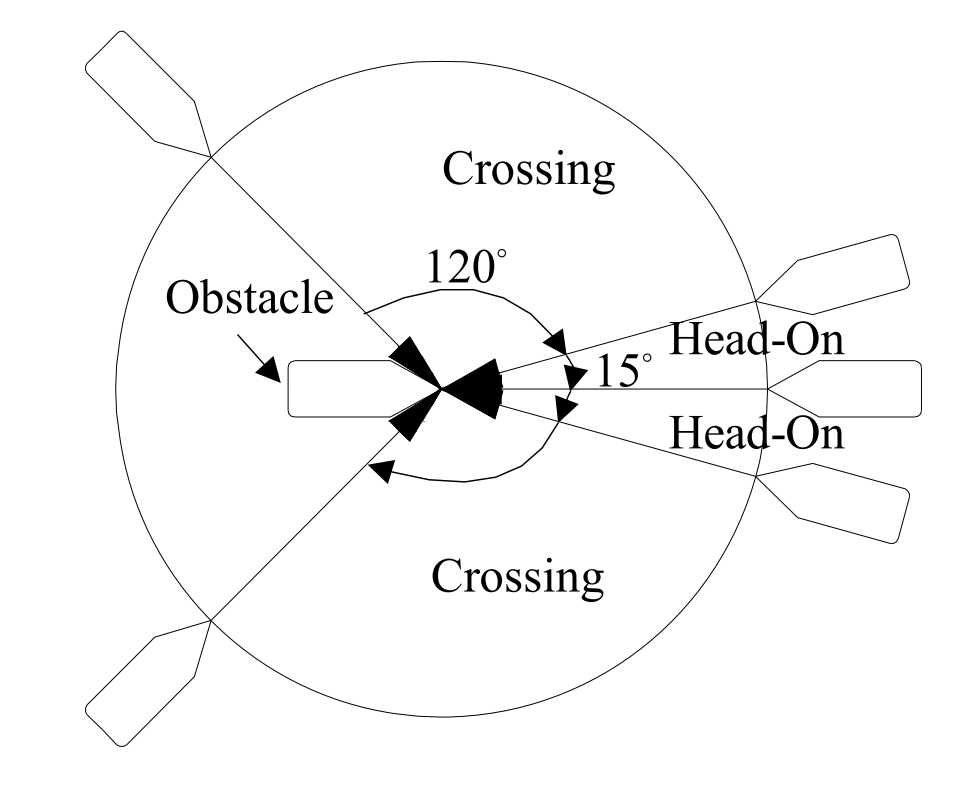
\includegraphics[scale=0.4]{figs/Chap3/Zhuang2011Motion_Sectors.png}
        \caption{Sectors for Identification of Dangerous Situation Type \cite{Zhuang2011Motion}}
        \label{fig:Zhuang2011Motion_Sectors}
    \end{figure}
    %%%%%%%%%%%%%%%%%%%%%%%%%%%%%%%%%%%%%%%%%%%%
    
    %%%%%%%%%%%%%%%%%%%%%%%%%%%%%%%%%%%%%%%%%%%% Svec2011
    \subsection{Svec 2011}
    For \ac{USV} trajectory definition, Svec \etal~\cite{Svec2011aAutomated, Svec2012Automated} present a automated guidance plan synthesis based on \ac{GP} method~\cite{Russel2003AI_GA}.
    % VJ explicar o que é isso bem rapidamente e atender o comentário acima do DJ :D
    % VJ Artigo relativamente importante, mas não me parece interessado em COLREGS.  Penso isso pelo termos usados: intruder... bloquear o avanço de intruder boats. Procede? Acho importante o artigo pois   existe um planejamento de alto nível.
    An initial version of a guidance plan is generated and then improved by detecting and fixing its shortcomings. The guidance plan is improved by data mining extraction of vehicle states of failure and then new iterations using \ac{GP}. Their solution is applied to the context of blocking the advancement of an intruder boat toward a valuable target. The guidance plan is represented as a composition of the navigation controller and a set of navigation plans.
    
    The navigation controller is composed of high-level navigation commands such as \textit{go-intruder-front}, \textit{turn-right}, \textit{turn-left}, and, \textit{go-straight}, conditional variables such as \textit{intruder-on-the-left/right/front/at-back}, \textit{intruder-has-target-on-the-left/right}, and \textit{usv-has-target-on-the-left/right}, standard \textit{boolean} values and operators such as \textit{if}, \textit{true}, \textit{false}, \textit{and}, \textit{or}, and \textit{not}, program blocks (seq2, seq3), and system commands (\textit{usv-sensor}, \textit{usv-velocity}, and \textit{usv-match-intruder-velocity})
    
    The navigation plan is composed of high-level navigation commands and program blocks.
    Leaves of the decision tree can be conditional variables or navigation commands.
    Inner nodes can be conditionals variables, navigation commands, or system commands.
    Figure \ref{fig:Svec2012Automated_GuidancePlanning} illustrates navigation controller and navigation plan.
    
    \begin{figure}[H]
        \centering
        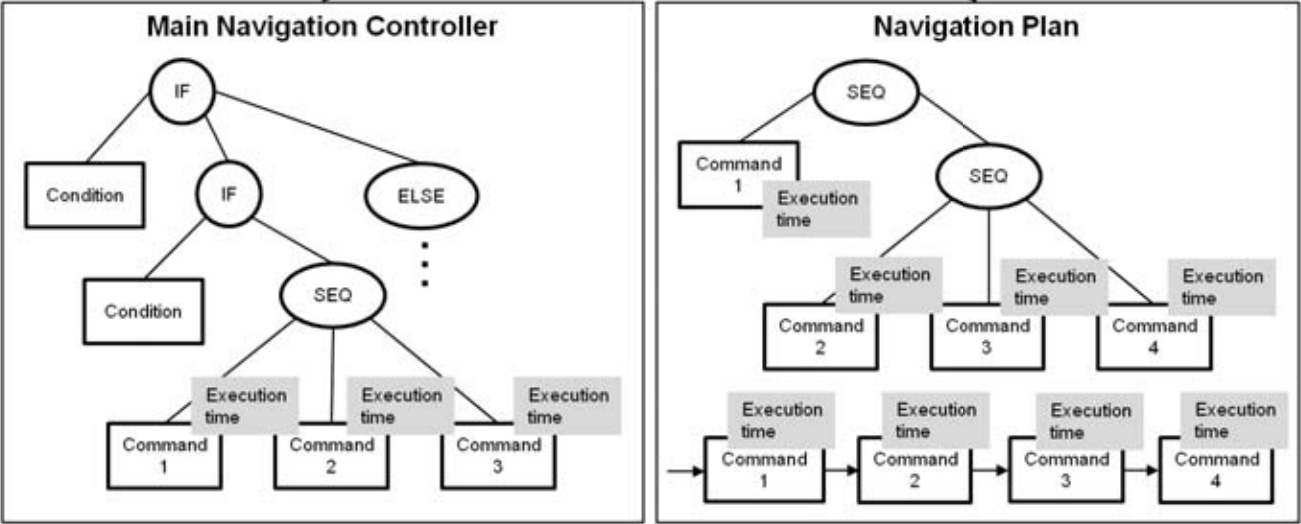
\includegraphics[scale=0.35]{figs/Chap3/Svec2012Automated_GuidancePlanning.png}
        \caption{Navigation controller and Navigation plan \cite{Svec2011aAutomated, Svec2012Automated}}
        \label{fig:Svec2012Automated_GuidancePlanning}
    \end{figure}
    %%%%%%%%%%%%%%%%%%%%%%%%%%%%%%%%%%%%%%%%%%%%
 
    %%%%%%%%%%%%%%%%%%%%%%%%%%%%%%%%%%%%%%%%%%%%  Soltan2009Trajectory
    \subsection{Soltan 2009 Trajectory}
    Soltan \etal~\cite{Soltan2009Trajectory} present the usage of \acp{ODE} for the approximation of the position of obstacles through the generation of elliptical fields around the obstacles. In this study, the \ac{USV} mission consists of following another target boat. The global guidance system tries to follow the target boat going towards it in a straight line. If any obstacle is detected, the local guidance system defines the trajectory around the obstacle considering the elliptical fields defined using \acp{ODE}. The evaluation of the system was done by simulation. They assumed that the \ac{USV} was capable of detecting any obstacle between the \ac{USV} and the target boat, in any range. Figure \ref{fig:Soltan2009Trajectory_SimulateTests_Ellipsses} shows two simulate scenarios where we can see elliptical fields for the approximation of 4 obstacles and the \ac{USV} trying to follow the target boat in 2 different scenarios.
    
    \begin{figure}[H]
        \centering
        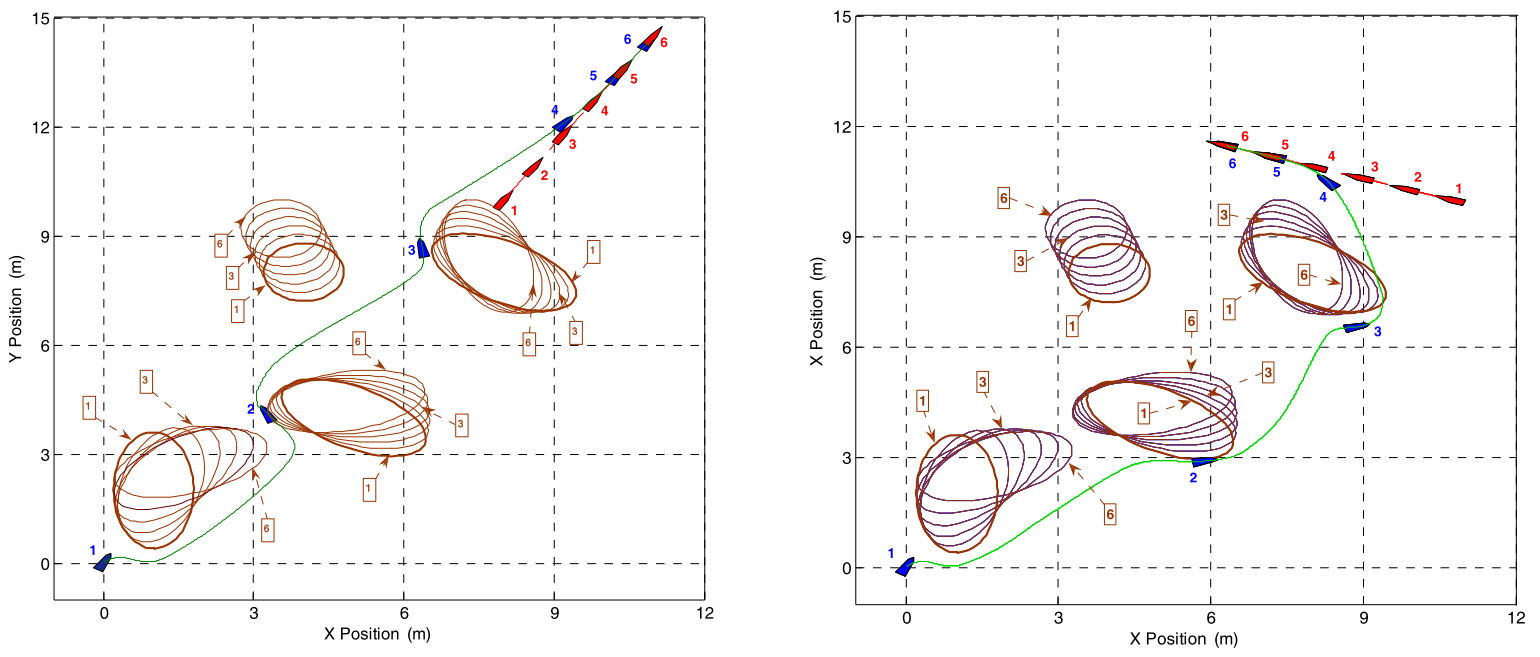
\includegraphics[scale=0.3]{figs/Chap3/Soltan2009Trajectory_SimulateTests_Ellipsses.png}
        \caption{Elliptical obstacles approximations \cite{Soltan2009Trajectory}}
        \label{fig:Soltan2009Trajectory_SimulateTests_Ellipsses}
    \end{figure}
    %%%%%%%%%%%%%%%%%%%%%%%%%%%%%%%%%%%%%%%%%%%% 
    
    %%%%%%%%%%%%%%%%%%%%%%%%% 
    %%%%%%%%%%%%%%%%%%%%%%%%% 2019 Reviews
    %%%%%%%%%%%%%%%%%%%%%%%%% 
    
    %%%%%%%%%%%%%%%%%%%%%%%%%%%%%%%%%%%%%%%%%%%% Abdelaal2017NMPC, Abdelaal2018Nonlinear 
    \subsection{Abdelaal 2017 NMPC}
    Abdelaal \etal~\cite{Abdelaal2017NMPC, Abdelaal2018Nonlinear} explore trajectory tracking controlling, based on \ac{MPC}. Trying to be COLREGS-compliant, their solution prioritizes maneuvering to the starboard side when in an encounter with obstacles, but this is not a suitable approach for real-world scenarios, as discussed before. They assume to be capable of detecting and identifying velocity, course, and length of other vessels, suggesting the use of \ac{LIDAR} and \ac{AIS} in tests on the field. The motion prediction of encountered vessels is made using a constant velocity model \cite{Rong2003Survey}. Obstacles are assumed to have a circular shape, and collision avoidance is translated into an inequality constraint, integrated into the controller design. The method is validated through software simulation using MATLAB.
    %%%%%%%%%%%%%%%%%%%%%%%%%%%%%%%%%%%%%%%%%%%%
    
    %%%%%%%%%%%%%%%%%%%%%%%%%%%%%%%%%%%%%%%%%%%% Benjamin2004COLREGS
    \subsection{Benjamin 2004 COLREGS}
    Benjamin \etal~\cite{Benjamin2004COLREGS} were pioneers in presenting a detailed discussion about the appliance of \ac{COLREGS} to USVs. Beyond, they present an overview of the "COLREGS project," showing simulation and field test modeling. Their strategy consisted of using a behavior-based control for the integration of \ac{COLREGS}-compliant collision avoidance and mission accomplishment.
    
    For \ac{COLREGS}-compliant global guidance, the output of each behavior is an objective function that rates all possible actions concerning the corresponding \ac{COLREGS}. So, they use interval programming to solve the multi-objective optimization problem. The \ac{COLREGS} behaviors rate possible vehicle actions in a decision space defined by the decision variables course, speed, and intended-time. Then, a not clearly defined shortest-path algorithm is run.
    
    For validation, they performed the test in simulation and field tests. In simulation, the controlled vehicle knows its own position perfectly, as well as the position and trajectory of all other moving vessels. They present the behavior related to the head-on situation. In the in-water experiments, the vehicle knows its position from GPS, and each vehicle broadcasts its GPS position to each other. Their experiment was performed using four 10-foot kayaks equipped with on-board computers running Linux and Mission Oriented Operating Suite\cite{MOOS}, GPS, compass, and a not clearly defined commercially available bathymetry map for the definition of free space.
    %%%%%%%%%%%%%%%%%%%%%%%%%%%%%%%%%%%%%%%%%%%%
    
    %%%%%%%%%%%%%%%%%%%%%%%%%%%%%%%%%%%%%%%%%%%% Huang2019Generalized 
    \subsection{Huang 2019 Generalized}
    Recently, some improvements have been made considering multi-ships dynamics. For example, Huang et al. \cite{Huang2019Generalized} present multi-vessel collision avoidance systems using an extension of the Velocity Obstacle algorithm, namely Generalized Velocity Obstacle, for local planning. Through software simulation, it is proved that the system is capable of avoiding multiple risks encounters with other vessels considering changes on course and speed and attending \ac{COLREGS} when possible. For \ac{COLREGS}-compliance, the system uses hard-port turn decision. Moreover, the authors argue that the system is suitable for both autonomous and officer support.
    
    \section{Literature Discussion}
    
    %% Grammarly 100/100
    In this section, we briefly discuss important aspects related to the development of \ac{USV} guidance and collision avoidance systems presented in the literature. Based on the read studies, we can have a glance about the relevance of A*, \ac{LOS}, and \ac{VO} for \ac{USV} guidance and the focus on addressing avoidance of overtaking, head-on, and crossing collision situations.
    
    
    %\subsection{Guidance}
    %AMA  nao faz sentido ter uma secao somente
    
    %% Grammarly 100/100
    In general, guidance based on path planning requires addressing both stationary and dynamic obstacles. Regarding real-world-tested work, guidance requires an accurate world model and robust methods to avoid detected obstacles. World representation is done using cost maps and information is collected through nautical charts~\cite{Larson2006Autonomous}, electronic charts~\cite{Naus2013Idea}, \ac{ARPA} contacts~\cite{Larson2006Autonomous}, and \ac{AIS}~\cite{Abdelaal2017NMPC}. The usage of these two last allow path planning for global guidance to consider not only stationary obstacles but moving obstacles also. Regarding the location and orientation of the \ac{USV} itself, the analyzed literature presented the usage of GPS~\cite{Benjamin2004COLREGS} and compasses~\cite{Annamalai2013Comparison}. Based on our literature review we identified the following methods for global and local planning:
    
    \begin{enumerate}
    
        %% Grammarly 100/100
        \item Regarding global planning we identified the usage of the following methods: \ac{VO}~\cite{Larson2006Autonomous, Kuwata2014Safe, Zhuang2011Motion, Huang2019Generalized}, A*~\cite{Naeem2012COLREGS, Campbell2012Review_COLREGs, Naus2013Idea} e genetic programming~\cite{Svec2012Automated, Svec2011aAutomated}. The works that presented A* and VO for global planning achieved proper behavior, being capable of planning and avoiding collision in the scenarios presented by the authors. At the same time, the usage of optimization methods (\ie~genetic programming) implied limitations due to the high cost for real-time applications. 
        
        %% Grammarly 100/100
        \item Regarding local planning we identified the usage of the following methods: A*\cite{Larson2006Autonomous, Campbell2013Automatic, Agrawal2015COLREGS}, \ac{VO}~\cite{Larson2006Autonomous, Huang2019Generalized}, \ac{LOS}~\cite{Naeem2012COLREGS}, and Virtual Force Field~\cite{Lee2004Fuzzy}. Also, the review presented by Liu \etal~\cite{Liu2016Unmanned} indicates the usage of potential fields~\cite{Healey2007Collaborative, Soltan2009Trajectory}. Regarding \ac{COLREGS} compliance, the heuristics solutions were based on search space restriction while the solutions presented by  Naeem~\etal~\cite{Naeem2012COLREGS}, Lee~\etal~\cite{Lee2004Fuzzy}, consisted in performing a hard turn to the starboard side in every detected encounter between vessels. We consider this is not a good approach since this action may lead to violation of other \ac{COLREGS} rules such as rule 10 that impose that navigation must respect \acf{TSS}.
        
    \end{enumerate}
    
    %Grammarly 97/100
    Collision avoidance is performed mostly with an architecture composed of two subsystems, one deliberative and other reactive. Deliberative systems are based on well-known maps and are implemented through optimization and heuristics methods. Reactive systems run online, are based on real-time collected data from \ac{LIDAR}~\cite{Agrawal2015COLREGS}, \ac{SONAR}~\cite{Candeloro2017Voronoi}, and cameras\cite{Kuwata2014Safe} and requires more intelligent systems since they must be compliant to protocols such as the \ac{COLREGS}. 
    
    Based on the literature, the identification of \ac{COLREGS} situation can be made through the calculation of the bearing angle~\cite{Kuwata2014Safe}\footnote{We use it in our system and explain it in chapter~\ref{chap:4_COLREGS_Compliant_Guidance_System}}. Some authors present the usage of \ac{CPA}~\cite{Campbell2013Automatic} for anticipated detection of \ac{COLREGS} situation while other authors present purely reactive approaches.
    
    Relevant work that applied and tested their techniques on real-world situations worked on using a well-known method, such as A* and \ac{VO}, and applied some constraints on the search space of action to make them \ac{COLREGS}-compliant \cite{Kuwata2014Safe, Campbell2013Automatic}. 
    The \ac{COLREGS}-compliant systems presented in the literature were evaluated through software simulation~\cite{Soltan2009Trajectory, Abdelaal2017NMPC, Benjamin2004COLREGS, Lee2004Fuzzy} as well as field tests~\cite{Agrawal2015COLREGS, Benjamin2004COLREGS, Kuwata2014Safe}.
    
    One of the challenges involving \ac{COLREGS} is related to the fact that the rules were defined expecting a large amount of human intuition and experience to fulfill gaps and non-objective rules descriptions. For example, the vague definition of angles and distances that must be respected generate non-standard parameters definition. Studies explicitly declare that these parameters were empirically defined after several tests \cite{Larson2007Advances}, but these definitions not necessarily solve the problem for \ac{USV} of different sizes and capabilities, generating a generalization problem.
    
    %AMA favor usar https://www.grammarly.com/. usa esse user moraesfg@gmail.com e essa senha 'moraes65'. depois de usar, apaga o arquivo gerado.
    
    
    
    
    
    % \section{Literature Discussion}
    
    % In this section, we briefly discuss important aspects related to the development of \ac{USV} guidance and collision avoidance systems presented in the literature. Table \ref{tab:RelatedWork_Summary} presents a summary of the methods used for implementation of guidance system path planners and the addressed \ac{COLREGS} rules. Based on read studies, we can have a glance about the relevance of A*, \ac{LOS} and \ac{VO} for \ac{USV} guidance and the focus on addressing avoidance of overtaking, head-on and crossing collision situations.
    
    % \begin{table}[H]
    % \caption{Literature guidance methods and applied COLREGS rules summary}
    % \label{tab:RelatedWork_Summary}
    % \begin{tabular}{l|c|c|c|c}
    % \hline
    % \multicolumn{1}{c}{Studies}            & Global & Local & Hybrid & \multicolumn{1}{c}{COLREGS-compliance (Rules)}   \\ \hline
    % \hline
    % \cite{Larson2006Autonomous}                     & A*              & Arcs           &                 &                                                          \\
    % \cite{Naeem2012COLREGS}                         & DPSS            & LOS            &                 & 6, 8,  14, and 15, and 16                                \\
    % \cite{Campbell2013Automatic}                    & A*              & R-RA*          &                 & 6, 8, 13, 14, 15, and 16                                 \\
    % \cite{Naus2013Idea}                             & A*              &                &                 &                                                          \\
    % \cite{Annamalai2013Comparison}                  & LOS             &                &                 &                                                          \\
    % \cite{Lee2004Fuzzy}                             &                 & VFF + Fuzzy    &                 & 6, 8, 13, 14, 15, 16, and 17                             \\
    % \cite{Kuwata2014Safe}                           &                 & VO             &                 & 6, 8, 13, 14, 15, and 16                                 \\
    % \cite{Benjamin2006Method}                       &                 & Behavior       &                 & 14                                                       \\
    % \cite{Zhuang2011Motion}                         & Evolutionary    & VO             &                 & 14, 15, and 16                                           \\
    % \cite{Svec2011aAutomated, Svec2012Automated}    &                 &                & GP              &                                                          \\
    % \cite{Soltan2009Trajectory}                     &                 &                & ODE             &                                                          \\ \hline
    % \end{tabular}
    % \end{table}
    
    % In addition to the presented studies, the survey presented by Liu \etal~\cite{Liu2016Unmanned} highlights the following studies and methods for guidance and collision avoidance: 
    % A* \cite{Svec2011Trajectory, Svec2012USV}; 
    % \ac{LOS} \cite{Breivik2008Straight, Caccia2008Basic, Caccia2005Sampling, Desa2007Small, Fredriksen2006Global, Naeem2012Integrated, Peng2013Adaptive, Sharma2013Genetic, Xu2007Multi};
    % Potential Fields \cite{Healey2007Collaborative, Soltan2009Trajectory}; and
    % Near-field reactive control \cite{Larson2007Advances}.
    
    % % Discussion about guidance
    % % VJ Darlan, as 2 subsections abaixo estão curtas e misturadas em termos de conteúdo. Vc explica path planning for guidance... quando o título é guidance. Depois vc explica que collision avoidance requer blah blah. Talvez remover as subsections desta sessão te ajude a deixar o texto mais fluído.
    % \subsection{Guidance}
    % In general, Guidance based on path planning requires to address both stationary and dynamic obstacles. Focusing on real-world tested work, guidance requires accurate world model and robust methods to avoid obstacles detected. World representation is done using occupancy grid and information is collected through nautical charts, electronic charts, \ac{ARPA} contacts, and \ac{AIS} contacts. The usage of these two last allow path planning for global guidance to consider not only stationary obstacles but moving obstacles also.
    
    % % Discussion about collision avoidance
    % \subsection{Collision Avoidance}
    % Collision avoidance is performed mostly with an architecture composed of two subsystems, one deliberative and other reactive. Deliberative systems are based on well-known maps and are implemented through optimization and heuristics methods. Reactive systems run online, are based on real-time collected data from \ac{LIDAR}, \ac{SONAR}, and cameras and requires more intelligent systems since they must be compliant to protocols such as the \ac{COLREGS}.
    
    % % Discussion about \ac{COLREGS}
    % % Vc implementa as COLREGS? Ou um método de planejamento para seguir COLREGS?
    % % DJ: Done
    % \subsection{COLREGS}
    % \ac{COLREGS}-compliant methods implementation involves definition of USV geometric constraints as shown in Figure \ref{fig:Zhuang2011Motion_Sectors} and \acf{CPA} for identification of which possible dangerous situation must be avoided. 
    % Relevant work that applied and tested their techniques on real-world situations worked on using a well-known method, such as A* and \ac{VO}, and applied some constraints on the search space of action to make them \ac{COLREGS}-compliant \cite{Kuwata2014Safe, Campbell2013Automatic}. 
    % In general, the \ac{COLREGS}-compliant systems presented in the literature were evaluated through software simulation without being tested on field guiding real boats.
    
    % One of the challenges involving \ac{COLREGS} is related to the fact that the rules were defined expecting a large amount of human intuition and experience to fulfill gaps and non-objective rules descriptions. 
    % % parece que vc vai citar outros quando vc diz one of the challenges, mas o parágrafo termina
    % For example, the vague definition of angles, and distances that must be respected generate non-standard parameters definition. Studies explicitly declare that these parameters were defined after several tests \cite{Larson2007Advances} but these definitions not necessarily solve the problem for \ac{USV} of different size and capabilities, generating a problem of generalization.
    
    % %AMA favor usar https://www.grammarly.com/. usa esse user moraesfg@gmail.com e essa senha 'moraes65'. depois de usar, apaga o arquivo gerado.
    
    % Relacionada a guidance, apresentamos abaixo as técnicas apresentadas na literatura para global planning e local planning. 

    % \begin{enumerate}
    %     \item Global planning: A partir da revisão da litaratura apresentada, observamos a utilização dos métodos \ac{VO}~\cite{Larson2006Autonomous, Kuwata2014Safe, Zhuang2011Motion, Huang2019Generalized}, A*~\cite{Naeem2012COLREGS, Campbell2012Review_COLREGs, Naus2013Idea} e genetic programming~\cite{Svec2012Automated, Svec2011aAutomated}. The works that presented A* and VO for gloabl planning, achieved suitable behavior, being capable to plan and avoid collision in the scenarios presented by the authors. While, the usage of optimization methods (\ie genetic programming) implied limitations due to the high cost for real-time application. 
        
    %     \item Local planning: A partir da revisão da literatura apresentada, observamos a utilização dos métodos A*\cite{Larson2006Autonomous, Campbell2013Automatic, Agrawal2015COLREGS}, \ac{VO}~\cite{Larson2006Autonomous, Huang2019Generalized}, \ac{LOS}~\cite{Naeem2012COLREGS}, and Virtual Force Field~\cite{Lee2004Fuzzy}. In addition, the review presented by Liu \etal~\cite{Liu2016Unmanned} indicate the usage of potential fields~\cite{Healey2007Collaborative, Soltan2009Trajectory}. Regarding COLREGS compliance, the heuristics solutions were based on search space restriction while the solutions presented by  Naeem~\etal~\cite{Naeem2012COLREGS}, Lee~\etal~\cite{Lee2004Fuzzy}, consisted in perform a hard turn to the starboard side in every detected encounter between vessels.
    % \end{enumerate}
\chapter{COLREGS Compliant Guidance System}
\label{chap:4_COLREGS_Compliant_Guidance_System}

    Is this chapter we present and describe the architecture of the \ac{USV} system we developed.

\section{Assumptions and Limitations}

    \begin{enumerate}
        
        %%%%%%%%%%%%%%%%%%%%%%%%
        % Grammarly: 100/100
        %%%%%%%%%%%%%%%%%%%%%%%%
        \item Encountering between power-driven vessels: we developed our system to run on power-driven vessels and considered the encountering between vessels of the same type. Concerning COLREGS, the encounter between different types of vessels imposes different ways to avoid collisions. Our system, in its current state, may be able to avoid collision with other vessels, but the avoidance strategy will always consider the other vessel as a power-driven vessel.

        %%%%%%%%%%%%%%%%%%%%%%%%
        % Grammarly: 95/100
        %%%%%%%%%%%%%%%%%%%%%%%%
        \item Encountering with one vessel: currently, we developed our system to perform COLREGS-compliant collision avoidance with only one vessel at a time. In a multiple vessels encounter scenario, our system may be able to perform evasive actions but we do not have any assurance regarding COLREGS-compliance for this scenario.

    \end{enumerate}

\section{System Architecture}

    %%%%%%%%%%%%%%%%%%%%%%%%
    % Grammarly: 100/100
    %%%%%%%%%%%%%%%%%%%%%%%%
    Our system consists of 3 main modules: guidance, navigation, and control. In Figure \ref{fig:gnc_arch}, we present an overview of the system.
    %Além dos módulos que compõem o nosso sistema são apresentados módulos externos ao \ac{USV} que são responsáveis pelo comportamento simulado do USV\_SIM e pelo 

    \begin{figure}
        \centering
        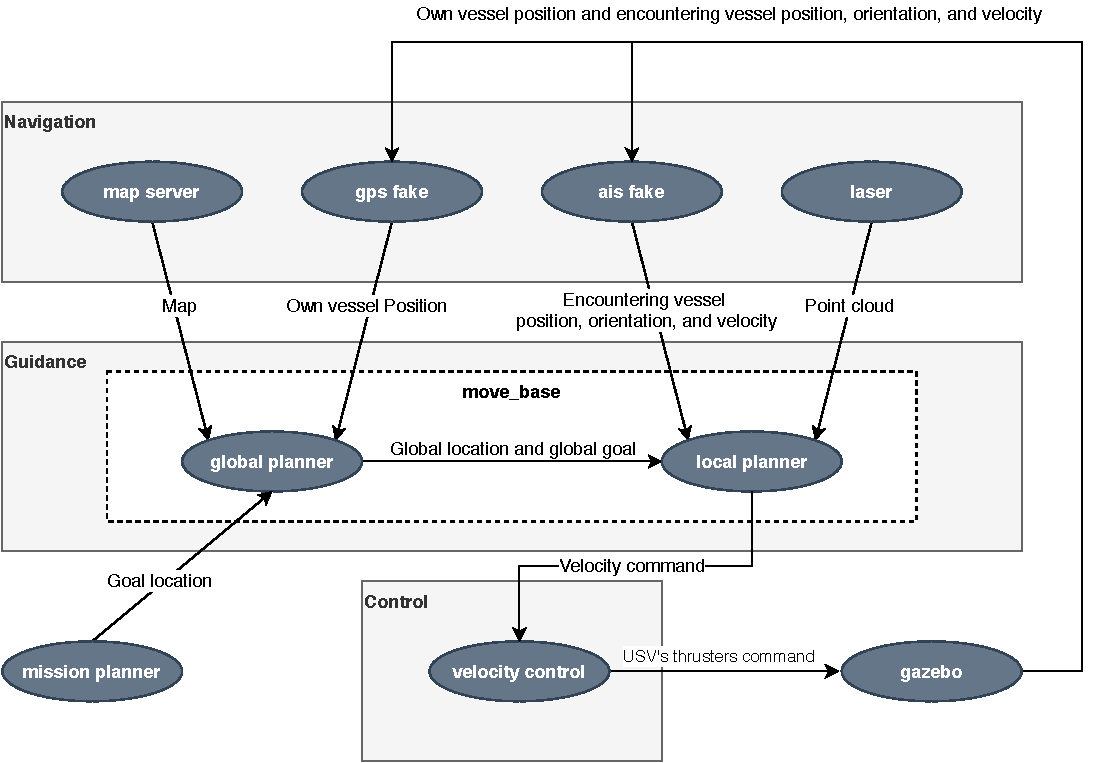
\includegraphics[scale=0.75]{figs/Chap4/gnc_arch.pdf}
        %%%%%%%%%%%%%%%%%%%%%%%%
        % Grammarly: 100/100
        %%%%%%%%%%%%%%%%%%%%%%%%
        \caption{Guidance, Navigation, and Control System Architecture: Beyond the GNC components of our system, we show in this Figure the mission\_planner and gazebo modules. The mission\_planner module is responsible for generating location goals to be followed by our \ac{USV}. The mission\_planner is currently an independent ROS-package; we developed it as an external module; this way, it can be replaced by any other module compliant to ROS publishing. The gazebo module is a general module for interacting with the simulator; through it, we can change and gather the \ac{USV} and the environment state.}
        \label{fig:gnc_arch}
    \end{figure}
    
    \subsection{Guidance}
    
        As shown in Figure \ref{fig:gnc_arch} the guidance module is mainly composed of global and local planner. Both planners are implemented inside the ROS move\_base environment. Fr global planning we use the move\_base standard A* search and for local planning we developed our own ROS move\_base plugin. This way we created our COLREGS-compliant local path planner and kept ROS compatibility.

        \subsubsection{Local Planner}
        
            %%%%%%%%%%%%%%%%%%%%%%%%
            % Grammarly: 99/100
            %%%%%%%%%%%%%%%%%%%%%%%%
            The local planner module is responsible for the reactive behavior of the system; that is, when encountering unknown static or dynamic obstacles, this module must be able to generate a behavior to avoid collision and, if possible, stay aligned with the global route generated by the global planner module.
        
            %%%%%%%%%%%%%%%%%%%%%%%%
            % Grammarly: 99/100
            %%%%%%%%%%%%%%%%%%%%%%%%
            In our system, the local planner module is responsible for COLREGS-compliant path planning. For COLREGS compliance, we adapted the usage of \ac{ATC} as presented by Agrawal \etal~\cite{Agrawal2015COLREGS}. With \ac{ATC}, we restrict the search space, building virtual obstacles in no COLREGS-compliant locations, see Figure \ref{fig:atc}.
            
            \begin{figure}[H]
            \centering
            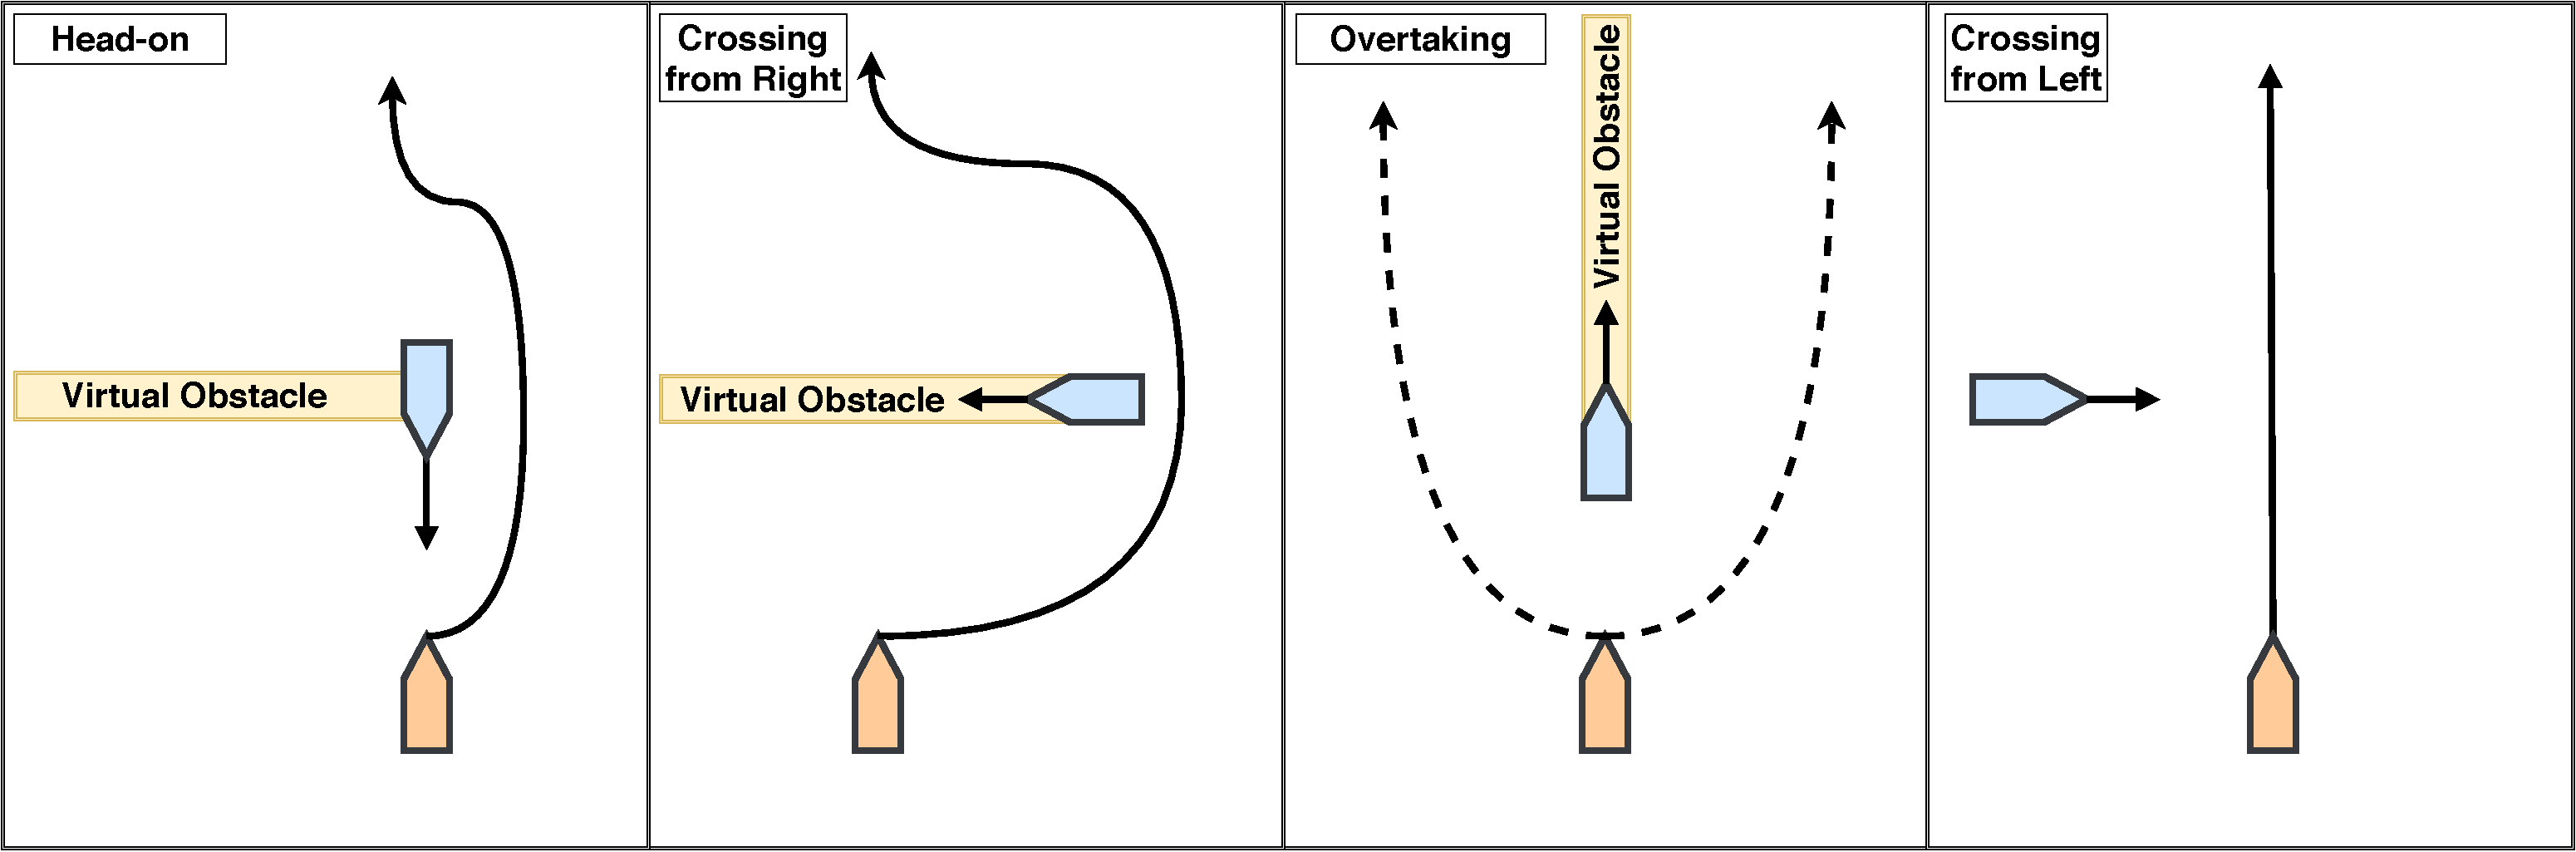
\includegraphics[scale=0.32]{figs/Chap4/atc.pdf}
            %%%%%%%%%%%%%%%%%%%%%%%%
            % Grammarly: 100/100
            %%%%%%%%%%%%%%%%%%%%%%%%
            \caption{\ac{ATC} for COLREGS Encounters: }
            \label{fig:gnc_arch}
        \end{figure}
        
        \begin{figure}[H]
            \centering
            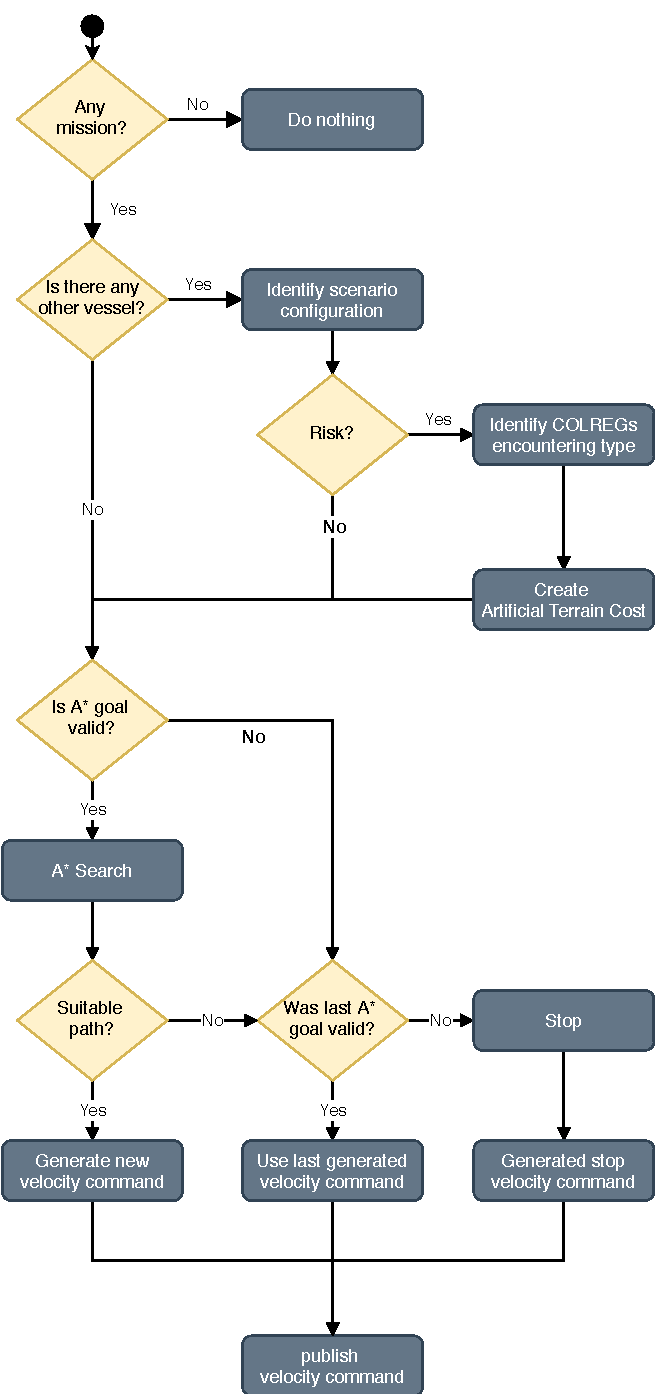
\includegraphics[scale=0.75]{figs/Chap4/AStartwithATC_flowChart.pdf}
            %%%%%%%%%%%%%%%%%%%%%%%%
            % Grammarly: 100/100
            %%%%%%%%%%%%%%%%%%%%%%%%
            \caption{Here we present a simplification of the sequential execution of our COLREGS-compliant path planning method. Some details are omitted to facilitate the general understanding of how our method works.}
            \label{fig:gnc_arch}
        \end{figure}

    \subsection{Navigation}
    The navigation system consists of the following sub-modules:
    
    \begin{itemize}
    
        %%%%%%%%%%%%%%%%%%%%%%%%
        % Grammarly: 99/100
        %%%%%%%%%%%%%%%%%%%%%%%%
        \item \textbf{map\_server}: the map\_server module is responsible for making the global map available for the guidance system. The map is generated before the start of the \ac{USV} mission. Both the map and an adapted version of the map\_server module were made available by the USV\_SIM maintainers.
    
        %%%%%%%%%%%%%%%%%%%%%%%%
        % Grammarly: 99/100
        %%%%%%%%%%%%%%%%%%%%%%%%
        \item \textbf{gps\_fake}: the gps\_fake module is a simplification of a real GPS; its information is extracted directly from the simulator; that is, it does not perform a simulated query to satellites. The gps\_fake module performs a simple query to the gazebo module in order to acquire a 3-tuple for determination of the position of the \ac{USV} in the global reference plane. This module can be replaced by another localization method, such as AMCL or a real GPS device. We developed and integrated this module into the system as a contribution to this work.
    
        %%%%%%%%%%%%%%%%%%%%%%%%
        % Grammarly: 99/100
        %%%%%%%%%%%%%%%%%%%%%%%%
        \item \textbf{ais\_fake}: the ais\_fake module is a simplification of the real AIS system \footnote{A real AIS module must respect NMEA legislation, refer to NMEA for specification: URL} which is used on vessels sailing on the high seas. The ais\_fake module provides the position and velocity of another vessel. The ais\_fake generate its information from a direct query to the simulator data. We developed and integrated this module into the system as a contribution to this work.
    
        %%%%%%%%%%%%%%%%%%%%%%%%
        % Grammarly: 100/100
        %%%%%%%%%%%%%%%%%%%%%%%%
        \item \textbf{laser}: this module provides the location of bodies of mass that reflect the laser light beam through an ordered 3-tuple. This module is available as a standard module in USV\_SIM. We configured this module to be compatible with the following requirements: laser beam range up to 25m and 360º detection capability; both specifications are compatible with real lasers, for example, the Slamtec RPLIDAR A3 laser \cite{RPLidarA3}.
    
    \end{itemize}
    
    % \subsection{Guidance}
    % O sistema de guidance é composto pelos seguintes submódulos:
    % \begin{itemize}
    %     \item \textbf{global\_planner}: O módulo global\_planner é responsável por .
    %     \item \textbf{local\_planner}: .
    % \end{itemize}
    
    \subsection{Control}
    
        %%%%%%%%%%%%%%%%%%%%%%%%
        % Grammarly: 100/100
        %%%%%%%%%%%%%%%%%%%%%%%%
        The control system consists of the control\_vel module. The control\_vel module interacts directly with the simulator and sends actuation commands to modify the state of \ac{USV}. The control\_vel module sends actuation commands from the speed commands received from the local planning module. This module is available as a standard module in USV\_SIM, and we used it without any modifications.


    
% VO because the algorithms collect all the velocities that result in collisions and present a set of collision-free velocities for human/machine, which facilitates human/machine to search for the best option.

% The advantages of the VO algorithms have been noticed by researchers in maritime engineering. The idea of VO algorithms had ap- peared in the 1980s, named as Collision Threat Parameter Area (CTPA) (Degre and Lefevre, 1981; Lenart, 1983). Subsequently, Pedersen et al. (2003) showed that this method can provide a better support for the Officer On Watch (OOW) in collision prevention comparing with tra- ditional Automatic Radar Plotting Aid (ARPA). Later on, a series of studies proposed to use VO/CTPA algorithms for collision avoidance in various scenarios, e.g. restricted waters (Szlapczynski and Szlapczynska, 2017), multiple-ship (Szlapczynski, 2008), incorporating with regulations (Zhao et al., 2016), and unmanned ship (Kuwata et al., 2014). In (Huang et al., 2018), the algorithms which presume the target-ship keeps constant velocity, are concluded as a special case of the VO algorithm, called linear VO (LVO) algorithm. Details about the existing applications of VO algorithms in the maritime domain are addressed in Section 2.3.
\chapter{Simulation and Results}
\label{chap:5_Simulation_And_Results}
        
    % Grammarlly: 100/100
    In this chapter, we present simulation scenarios for qualitative and quantitative evaluation of our system, as well as the experimental results. The simulations cover different encounters scenarios between two vessels, one using our path planning method and other without any COLREGS-compliant method. For qualitative evaluation, we analyzed avoidance success and the behavior of our system when exposed to different environmental conditions. For quantitative evaluation, we analyzed the time for computation of our path planning method and the minimum distance kept between our COLREGS-compliant vessel and the encountering vessel during the simulation.

    \section{Simulations Characterization}

    % Grammarlly: 100/100
    We run our simulations on \usvsim\footnote{https://github.com/disaster-robotics-proalertas/usv\_sim\_lsa}~\cite{Paravisi2018Toward} simulator using the platform described in Table \ref{tab:simulation_platform_description}. 
    We developed 12 scenarios for evaluation the system focusing on being comparable with simulations presented in reference studies, \ie{} Agrawal \etal{} ~\cite{Agrawal2015COLREGS} and Huang \etal{} ~\cite{Huang2019Generalized}. We chose both studies for their quality (\ie{} h-index > 50) and similarity with our work. Agrawal \etal{} present our problem-solving inspiration but unfortunately, they do not present too much information about their system evaluation, so we based our tests and system evaluation on Huang \etal{} as they explicitly present their simulation scenarios characterization, results, and simulate a \ac{USV} similar to ours in the aspect of dimensions.
    
    \taburowcolors[1] 1{tableLineOne .. tableLineTwo}
    \tabulinesep = ^3mm_2mm
    \everyrow{\tabucline[.4mm  white]{}}

    \begin{table}[H]
        \caption{Simulation Platform Description}
        \centering
            \begin{tabu} to \textwidth { >{\bfseries}X[c, 0] X[c, 3]}
            \tableHeaderStyle
            Component & Specification \\
            Computer & Desktop Dell XPS 8700 \\
            Processor & Intel® Core™ i7-4770 CPU @ 3.40GHz × 8 \\
            Memory & \begin{tabular}[c]{@{}l@{}}Teikon PC3-12800u DDR3 1600 MHz 2GB x 2\\ Teikon PC3-12800u DDR3 1600 MHz 4GB x 2\end{tabular} \\
            Operating System & Ubuntu 16.04.6 LTS \\
            ROS Version & ROS Kinetic
            \end{tabu}  
        \label{tab:simulation_platform_description}
    \end{table}
    
    % Grammarlly: 100/100
    In our simulations, we use a differential boat - shown in Figure \ref{fig:diffboat} - with two thrusters, which enables it to rotate over its axis. This boat is modeled according to specifications of the Lutra Prop boat, acquired from Platypus ~\cite{PlatypusLLC}. Beyond the specifications shown in Table \ref{tab:diffboat_specs}, the Lutra boat we use in our simulation has a laser rangefinder for environment scanning in its bow. We set the rangefinder to be capable of detect objects in 25 meters in a range of 360°.
    
    % \taburowcolors[1] 1{tableLineOne .. tableLineTwo}
    % \tabulinesep = ^3mm_2mm
    % \everyrow{\tabucline[.4mm  white]{}}
    % \begin{table}
    %     \caption{Lutra Prop parameters}
    %     \centering
    %         \begin{tabu} to 0.45\textwidth { >{\bfseries}X[c, 2] X[c, 2]}
    %         \tableHeaderStyle
    %         Parameter       & Value       \\
    %         Length          & 106 cm      \\
    %         Width           & 48 cm       \\
    %         Height          & 15 cm       \\
    %         % Hull Volume     & ~0.02 $m^3$ \\
    %         Weight          & 9.7 Kg      \\
    %         % Extra Payload   & 3 Kg        \\
    %         % Thruster Force  & 22.54 N     \\
    %         % Linear drag     & 11.33       \\
    %         Maximum speed   & 1.41 m/s    \\
    %         \end{tabu}  
    %     \label{tab:simulation_platform_description}
    % \end{table}
    
    \begin{minipage}{\textwidth}
        \begin{minipage}[b]{0.35\textwidth}
        \centering
        \begin{figure}[H]
            \centering
            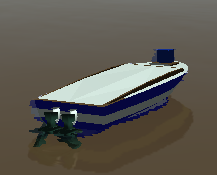
\includegraphics[scale=0.75]{figs/Chap5/diffboat.png}
            % \caption{Simulated version of Lutra Prop boat}
            % \label{fig:diffboat}
        \end{figure}
        \captionof{figure}{Simulated version of Lutra Prop boat}
        \label{fig:diffboat}
        \end{minipage}
    %   \hfill
        \begin{minipage}[b]{0.5\textwidth}
        \centering
            \begin{tabular}{cc}
                \toprule
                    \textbf{Parameter}       & \textbf{Value}       \\
                \midrule
                    Length          & 106 cm      \\
                    Width           & 48 cm       \\
                    Height          & 15 cm       \\
                    Weight          & 9.7 Kg      \\
                    Maximum speed   & 1.41 m/s    \\ 
                \bottomrule
            \end{tabular}
        \captionof{table}{Lutra Prop parameters}
        \label{tab:diffboat_specs}
        \end{minipage}
    \end{minipage}
    
    \vskip 1cm
    
     We assembled the scenarios in a simulated version of the Dilúvio stream. The Dilúvio stream is a potential location for real-world trials of our system due to the fact that it is near of our laboratory, so we evaluate the behavior of our system on a simulated version of it. In Figure \ref{fig:simulation_diluvio_googleLocation_roundedArea} we show with a red box the specific location we simulated in our experiments\footnote{Google maps location: (-30.047258°, -51.232660°), Av. Edvaldo Pereira Paiva, 1970 - Praia de Belas - Porto Alegre - RS - Brazil}. In Figure \ref{fig:simulation_diluvio_googleLocation2_roundedArea} we show side by side another perspective of the real-word location and its simulated version, in both Figures we marked with a red box a bridge region where we assembled some the encounters between the vessels.
     %AMA mencionar brevemente como esse cenario foi montado (foto area, resolucao de tanto, etc). O Marcelo tem essa descricao.
     
     As done by several authors, \eg{} Larson \etal{} ~\cite{Larson2006Autonomous}, Naeem \etal{} ~\cite{Naeem2012COLREGS}, Campbell \etal{} ~\cite{Campbell2013Automatic}, Naus ~\cite{Naus2013Idea}, \etc{}, we evaluated 4 main encounter scenarios between two vessels, head-on, crossing from right, crossing from left, and overtaking regarding COLREGS-compliance evaluation. In Figure \ref{fig:simulation_uwsim_headon_starting_pos} we show the starting configuration of the two vessel in a head-on encounter scenario, below the bridge shown in Figure \ref{fig:simulation_diluvio_googleLocation2_2_roundedArea}. Figures \ref{fig:simulation_uwsim_headon_starting_pos}, \ref{fig:simulation_uwsim_crossingright_starting_pos}, \ref{fig:simulation_uwsim_crossingleft_starting_pos} and \ref{fig:simulation_uwsim_overtake_starting_pos} show the starting configuration of the evaluated scenarios, the respective configuration of each scenario is presented in Tables \ref{tab:simulation_scenarios_configuration_own_vessel} and \ref{tab:simulation_scenarios_configuration_encountering_vessel}. 
     
     In this scenario the vessels encounter one another below the bridge presented in Figure \ref{fig:simulation_diluvio_googleLocation2_2_roundedArea}.
    
   \begin{figure}
        \centering
        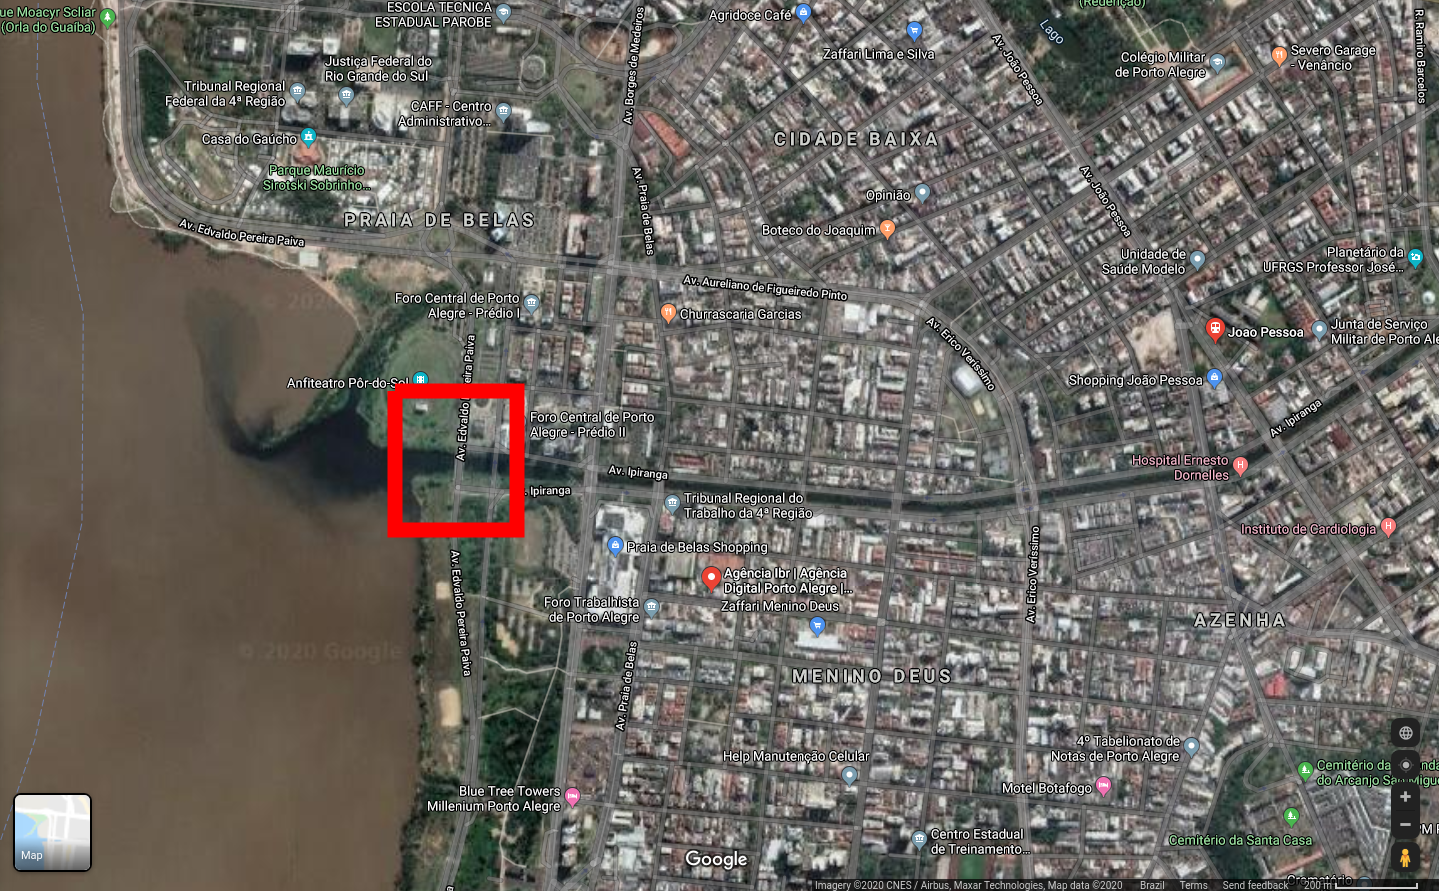
\includegraphics[scale=0.32]{figs/Chap5/simulation_diluvio_googleLocation_roundedArea.png}
        \caption{Real-world location of the area we choose for evaluation of our system.}
        \label{fig:simulation_diluvio_googleLocation_roundedArea}
    \end{figure}
    % \todo{cite some characteristics of the region}
    
    \begin{figure}
    \centering
        \begin{subfigure}[b]{0.48\textwidth}
            \centering
            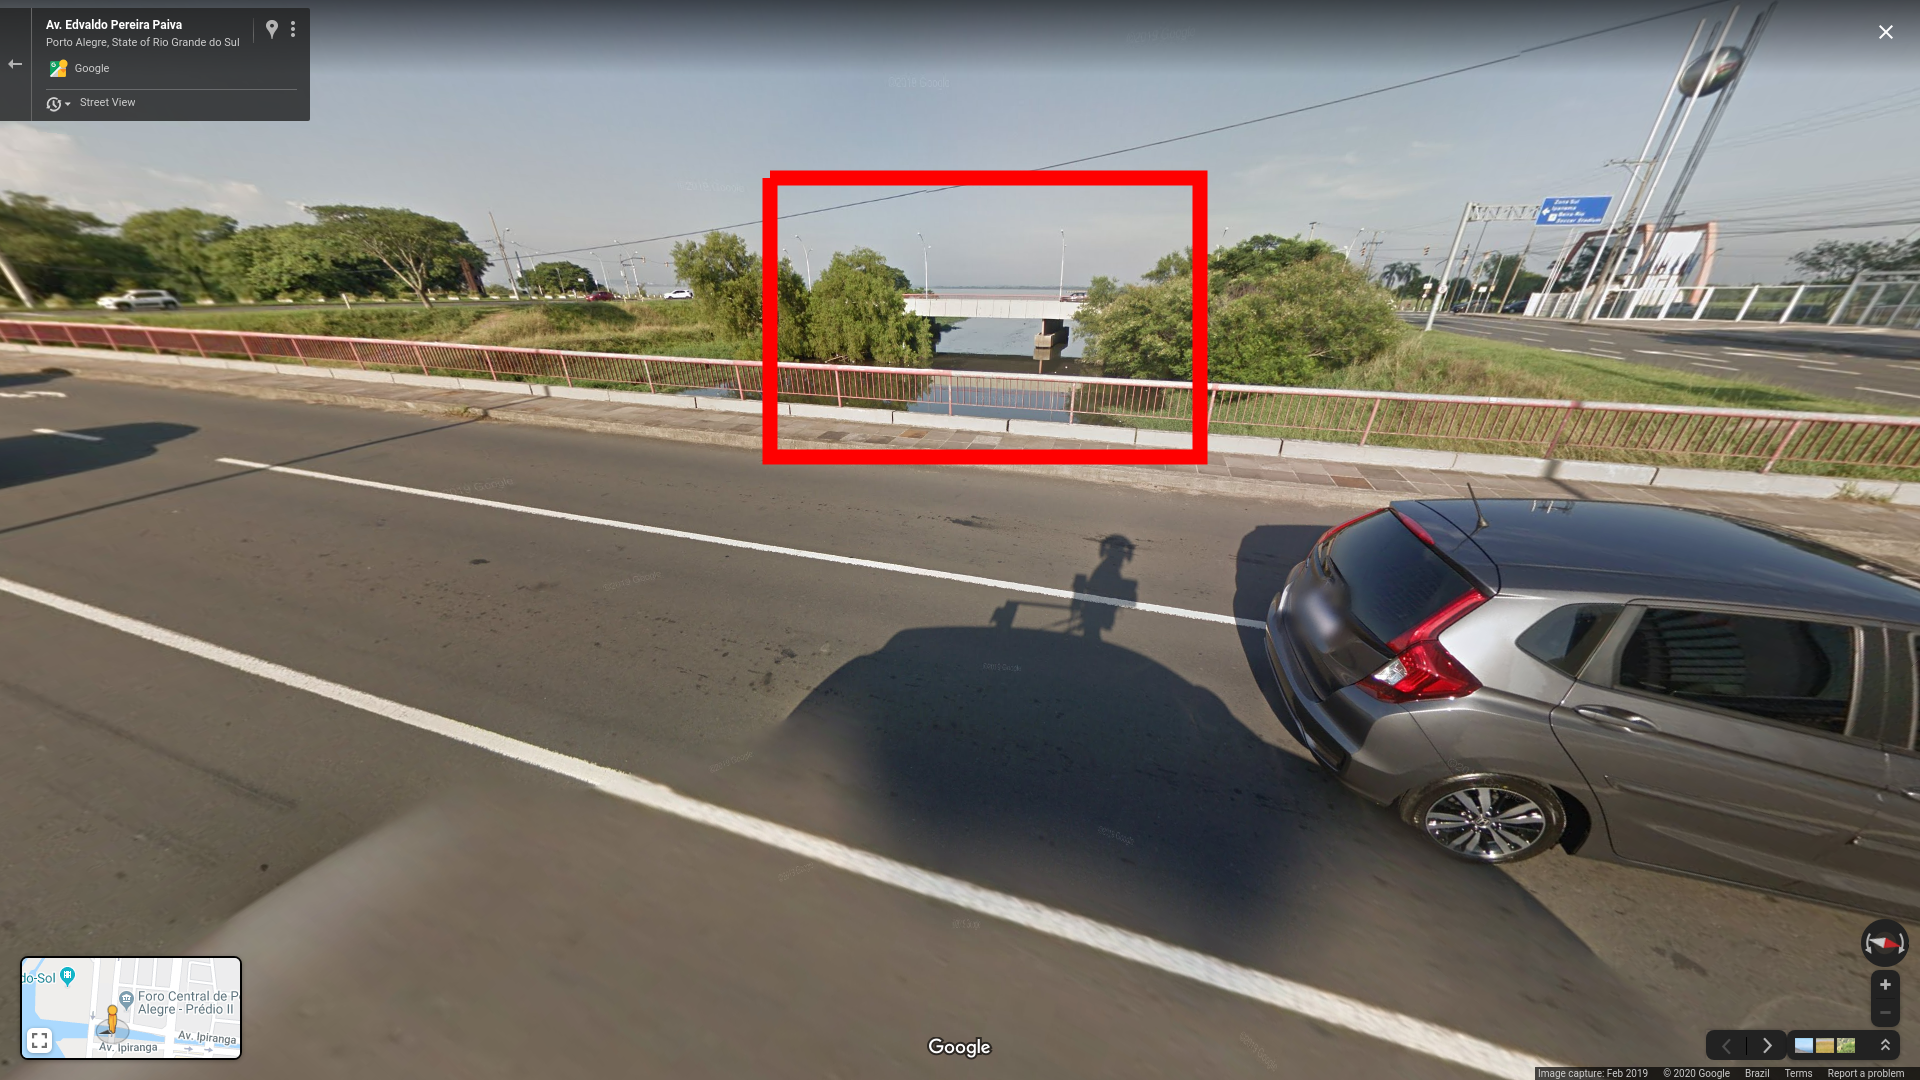
\includegraphics[scale=0.12]{figs/Chap5/simulation_diluvio_googleLocation2_1_roundedArea.png}
            \caption{Real World Location}
            \label{fig:simulation_diluvio_googleLocation2_1_roundedArea}
        \end{subfigure}
        \hfill
        \begin{subfigure}[b]{0.48\textwidth}
            \centering
            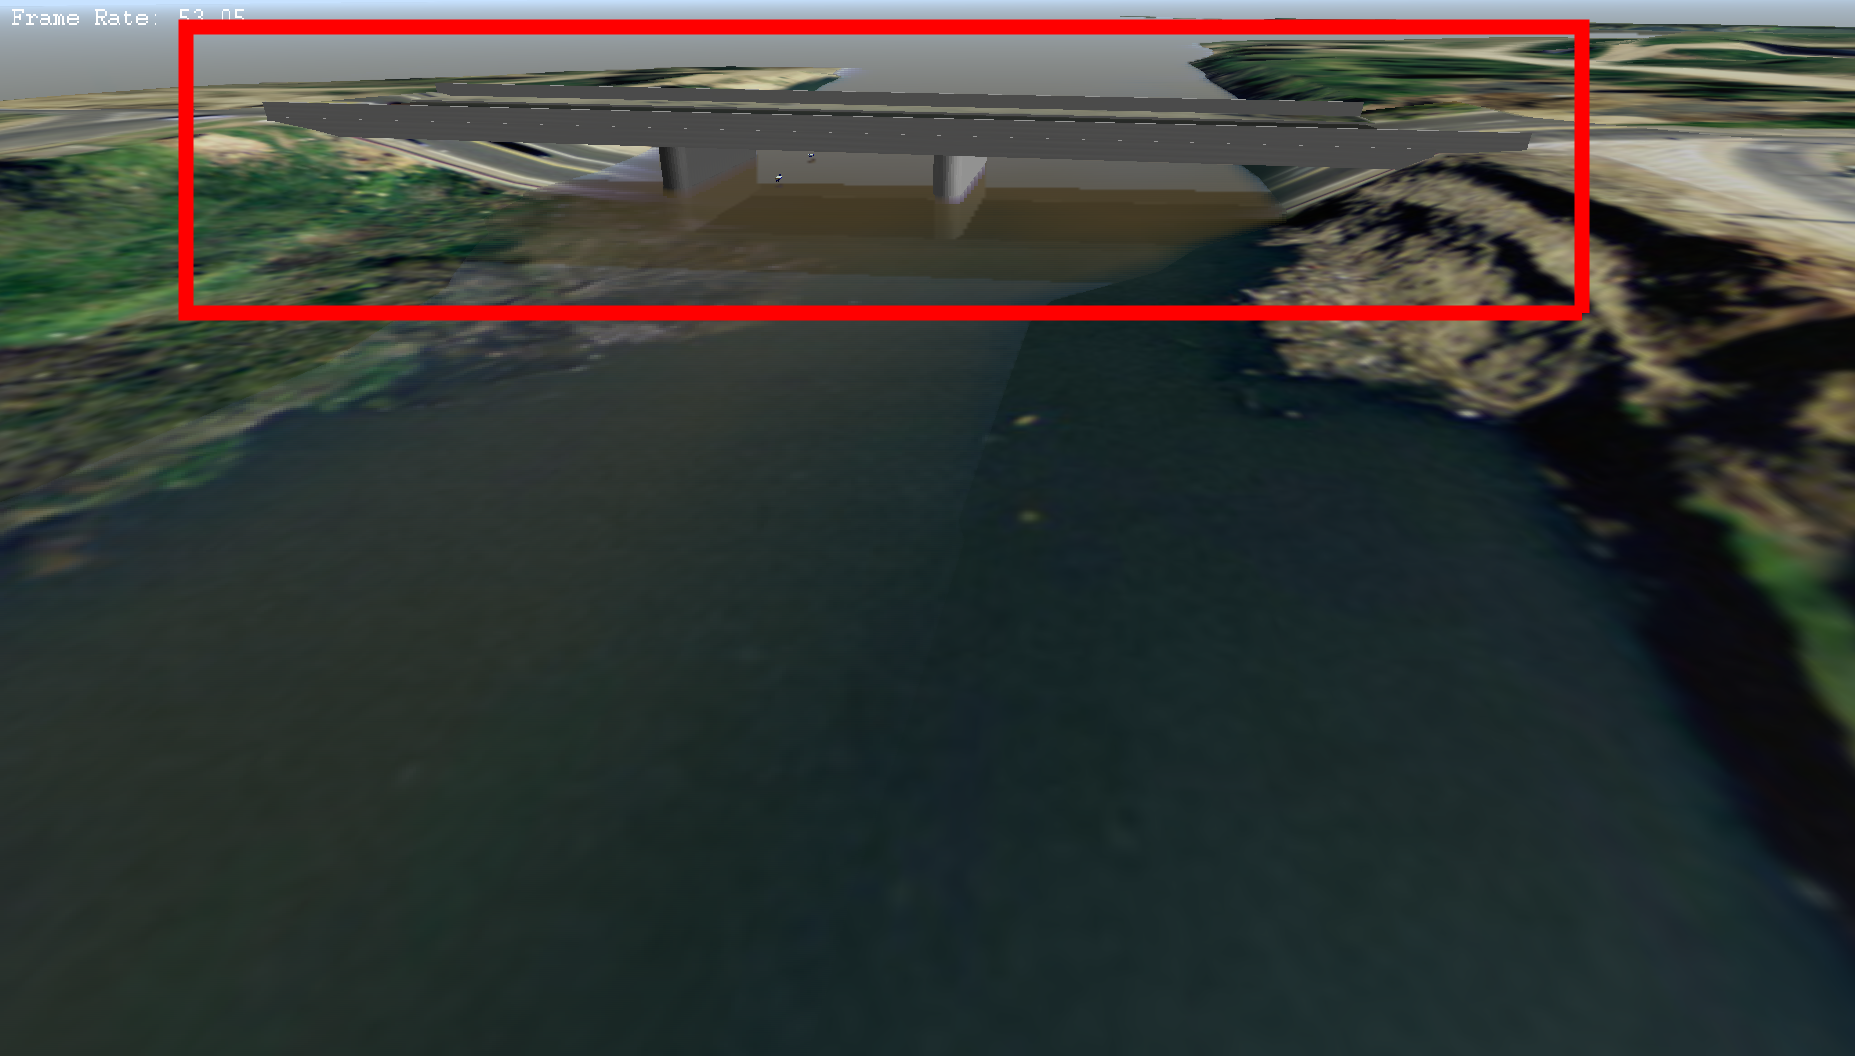
\includegraphics[scale=0.122]{figs/Chap5/simulation_diluvio_googleLocation2_2_roundedArea.png}
            \caption{Simulated version of Real World Location }
            \label{fig:simulation_diluvio_googleLocation2_2_roundedArea}
        \end{subfigure}
    
    \caption{Real world region and its simulated version}
    \label{fig:simulation_diluvio_googleLocation2_roundedArea}
    \end{figure}
    
    \begin{figure}[H]
    \centering
    
        \begin{subfigure}[b]{0.495\textwidth}
            \centering
            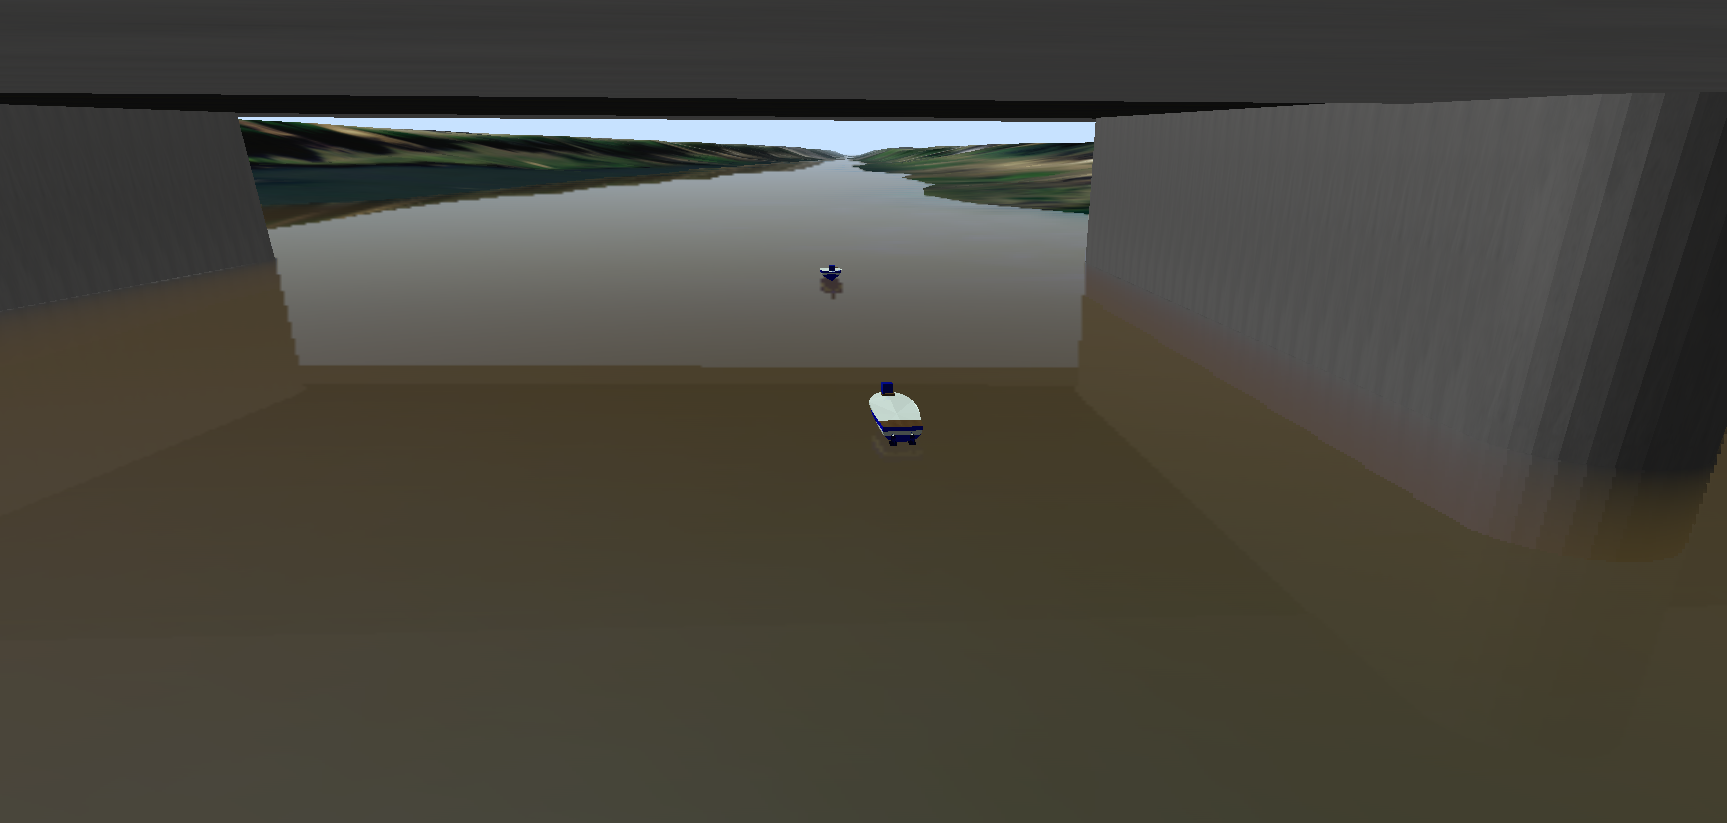
\includegraphics[width=\textwidth]{figs/Chap5/simulation_uwsim_headon_starting_pos.png}
            \caption{Head-on Encounter.}
            \label{fig:simulation_uwsim_headon_starting_pos}
        \end{subfigure}
        \begin{subfigure}[b]{0.495\textwidth}
            \centering
            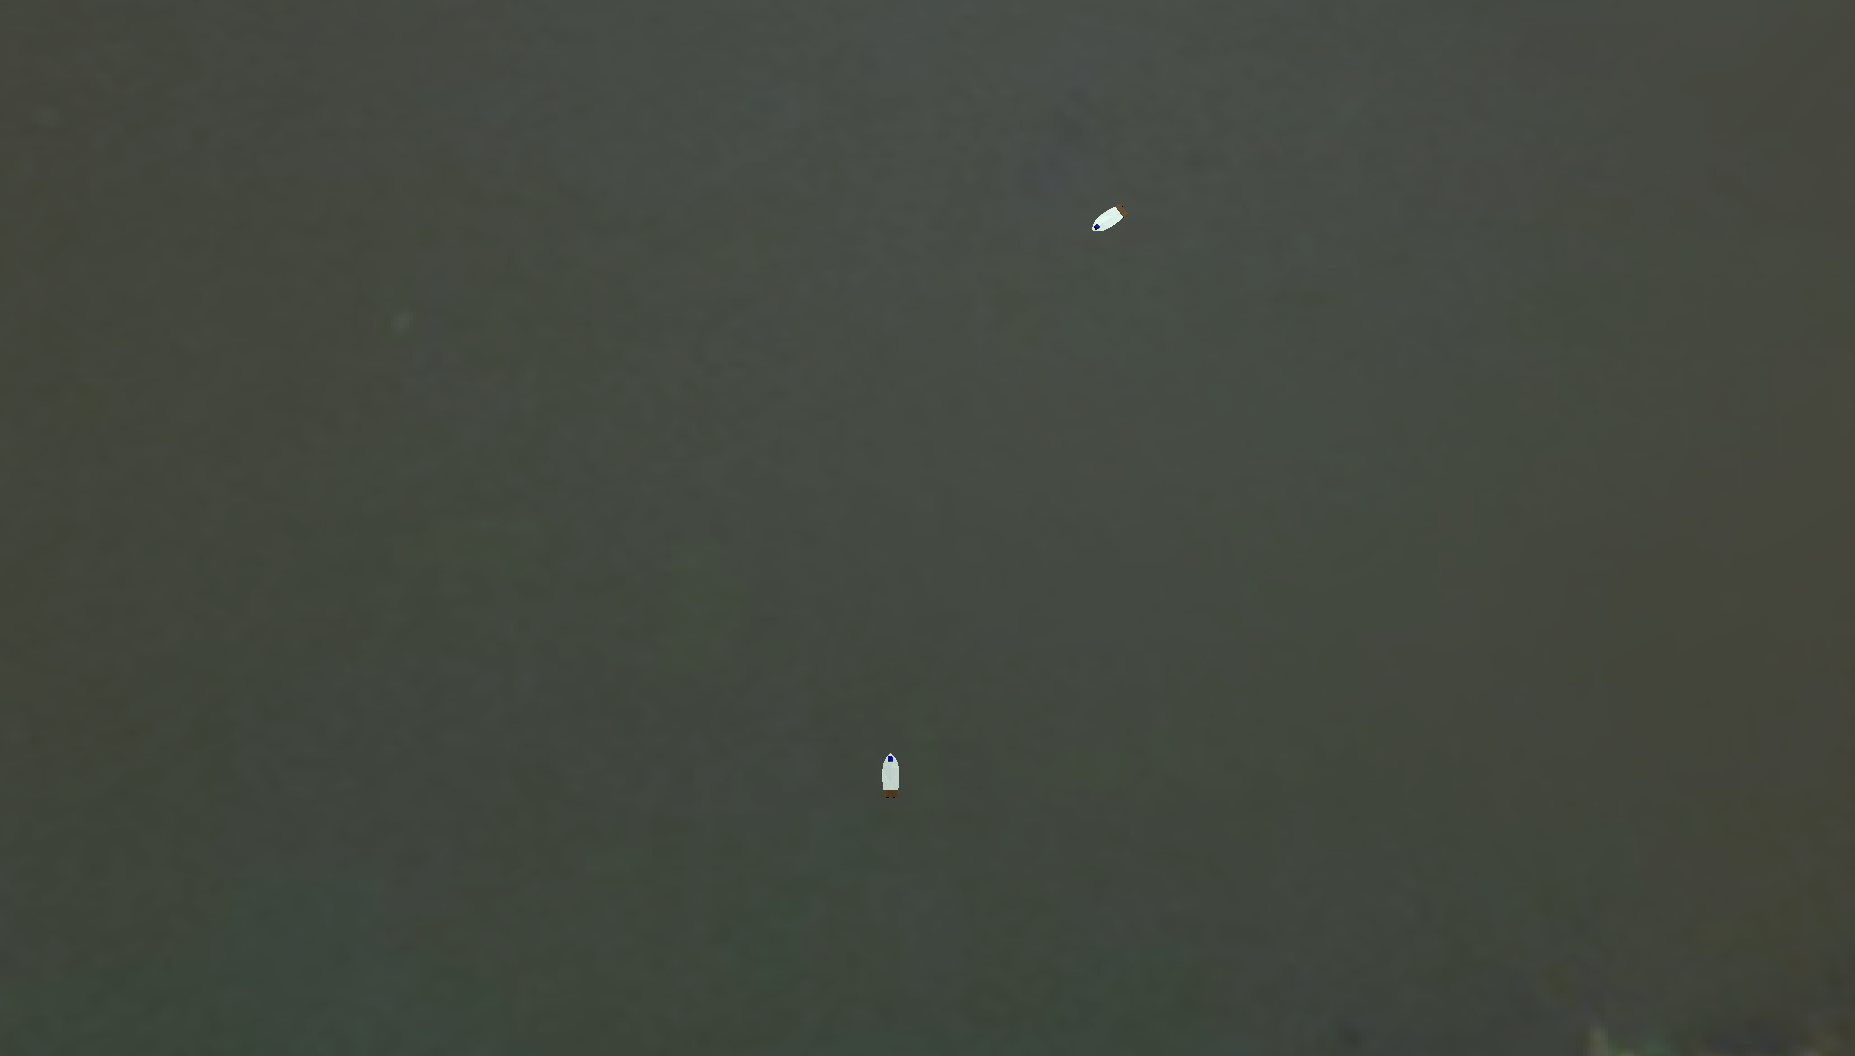
\includegraphics[width=\textwidth]{figs/Chap5/simulation_uwsim_crossingright_starting_pos.png}
            \caption{Crossing from Right}
            \label{fig:simulation_uwsim_crossingright_starting_pos}
        \end{subfigure}
        
        \begin{subfigure}[b]{0.495\textwidth}
            \centering
            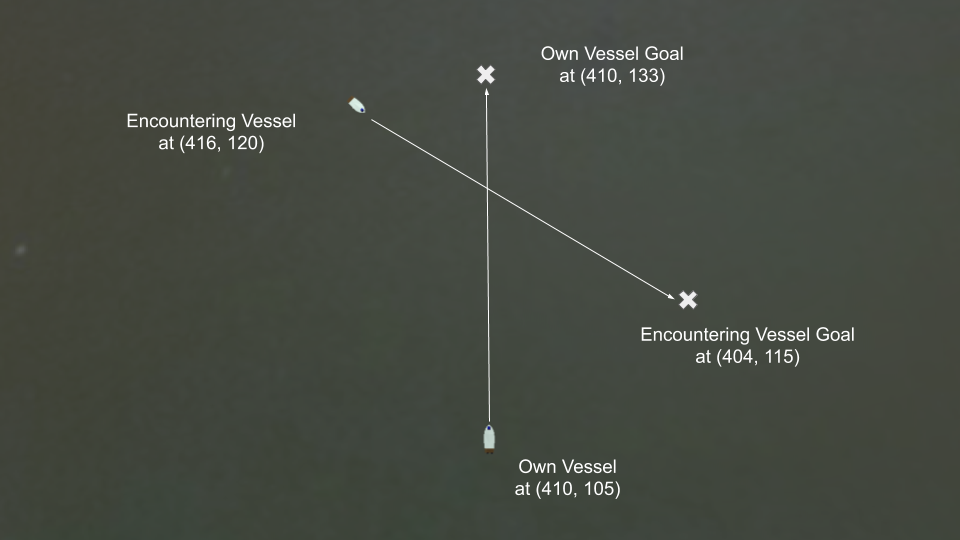
\includegraphics[width=\textwidth]{figs/Chap5/simulation_uwsim_crossingleft_starting_pos.png}
            \caption{Crossing from Left}
            \label{fig:simulation_uwsim_crossingleft_starting_pos}
        \end{subfigure}
        \begin{subfigure}[b]{0.495\textwidth}
            \centering
            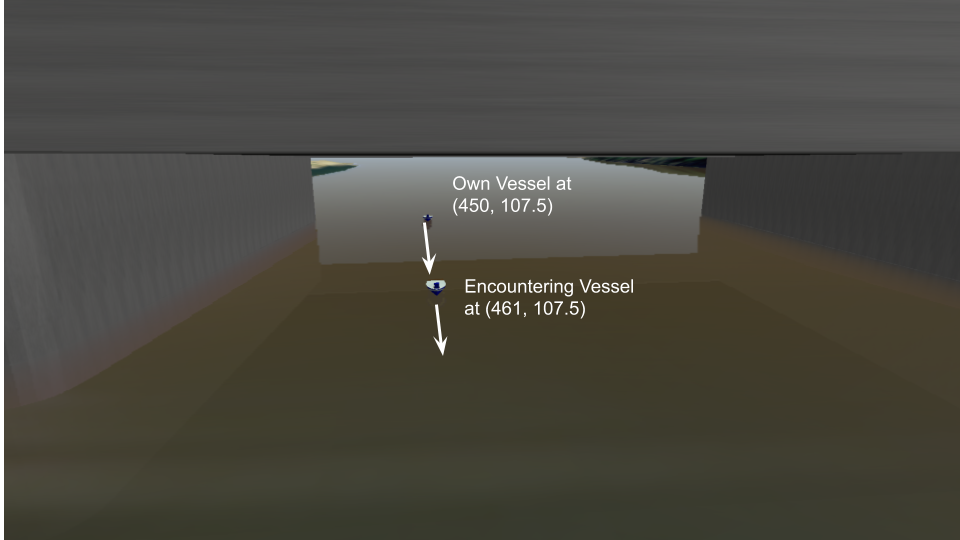
\includegraphics[width=\textwidth]{figs/Chap5/simulation_uwsim_overtake_starting_pos.png}
            \caption{Overtaking}
            \label{fig:simulation_uwsim_overtake_starting_pos}
        \end{subfigure}
    
    \caption{Encounter scenarios for evaluation. Scenarios adapted from ~\cite{Huang2019Generalized}.}
    \label{fig:simulation_uwsim_encounters}
    \end{figure}

%AMA o que siginifica OV na tab 5.3 ?
%DJ: Done

    \begin{center}
        \savebox{\mytablebox}{\begin{tabular}{cccc}
        
        \toprule[3pt]
        \multicolumn{4}{c}{\textbf{\acf{OV}}} \\
        % \multicolumn{3}{c}{\textbf{\ac{OV}}} \\
        \midrule
        \textbf{Encounter Type} & \textbf{Initial Pose (m, m, º)} & \textbf{Target Position} &  \textbf{Max. Speed (m/s)}\\
        \midrule
        Head On &  (450, 107.5, 0)  &   (480, 107.5)  &  0.47 \\
        Crossing Right &  (410, 105, 90)  &  (410, 133)  &  0.43  \\
        Crossing Left &  (410, 105, 90)  & (410, 133)   &  0.33  \\
        Overtaking &  (450, 107.5, 0)  &  (600, 107.5) &  0.5 \\
        \bottomrule
        
        \end{tabular}}
        \settowidth{\mytablewidth}{\usebox{\mytablebox}}
        \begin{minipage}{\mytablewidth}
        \captionof{table}{Encounter Scenarios Configuration and maximun achieved speed - \ac{OV}}
        \label{tab:simulation_scenarios_configuration_own_vessel}
        \usebox{\mytablebox}
        \end{minipage}

    \end{center}
    
    \begin{center}
        % \savebox{\mytablebox}{\begin{tabular}{cccc}
        \savebox{\mytablebox}{\begin{tabular}{cccc}
        
        \toprule[3pt]
        \multicolumn{4}{c}{\textbf{\ac{EV}}} \\
        % \multicolumn{3}{c}{\textbf{\ac{EV}}} \\
        \midrule
        \textbf{Encounter Type} & \textbf{Initial Pose (m, m, º)} & \textbf{Target Position} & \textbf{Max. Speed (m/s)}\\
        \midrule
        Head On &  (461, 107.5, 180)  &   (350, 107)  &  0.155 \\
        Crossing Right &  (416, 120, 215)  &  (404, 115)  &  0.1789  \\
        Crossing Left &  (404, 105, 315)  & (416, 115)  &  0.356  \\
        Overtaking &  (461, 107.5, 0)  &  (600, 107)  &  0.155 \\
        \bottomrule
        
        \end{tabular}}
        \settowidth{\mytablewidth}{\usebox{\mytablebox}}
        \begin{minipage}{\mytablewidth}
        \captionof{table}{Encounter Scenarios Configuration - \ac{EV}}
        \label{tab:simulation_scenarios_configuration_encountering_vessel}
        \usebox{\mytablebox}
        \end{minipage}

    \end{center}

    % Grammarlly: 100/100
    % Agrawal \etal ~\cite{Agrawal2015COLREGS} evaluate theirs A* approach in a 100mx100m grid with a resolution of 1:1, resulting in a search space of 10000 cells, we built our scenarios respecting the same proportionality. In all scenarios, our \ac{USV} plan in a 20mx20m grid with 1:0.2 resolution, resulting in a search space of 10000 cells, see Figure \ref{fig:rviz_local_costmap}. The choice of 20mx20m dimension is related to real limitations of the range and reliability on laser sensors, the RPLIDAR A3 laser~\cite{RPLidarA3} model, for example, is reliably capable of detection in 25 meters distance range.
    
    \section{Experiments Results}

        %%%%%%%%%%%%%%%%%%%%%%%%%%%%%%%%%%%%%%
        %% Intro to Experiments Results
        %
        %% Grammarlly: 93/100
        %% v2.0
        %%%%%%%%%%%%%%%%%%%%%%%%%%%%%%%%%%%%%%
        We qualitatively evaluated the behavior of our method in two different configurations. In the first configuration, we compare the behavior of the system with and without \ac{ATC}, and in the second configuration, we compare the behavior of our system with \ac{ATC} under the influence of wind and without the influence of wind. We executed both scenarios for four types of possible encounters between two vessels. For quantitative evaluation of each scenario, we measured the computation time of every execution of our path planner, average sustained speed, and minimal distance maintained between the vessels, as well as we evaluated whether the collision avoidance was successful or not. In Table \ref{tab:results} we summarize the collected results.

        %%%%%%%%%%%%%%%%%%%%%%%%%%%%%%%%%%%%%%
        %% Head-On w vs wo \ac{ATC}
        %
        %% Grammarlly: 99/100
        %%%%%%%%%%%%%%%%%%%%%%%%%%%%%%%%%%%%%%
        Figure \ref{fig:plot_ho_w_vs_wo} presents, comparatively, the final trajectory of two vessels in two executions of the same head-on scenario. For the \ac{OV}, the performed trajectory is guided by our local guidance system, and \ac{EV} from its start position must go to a goal ahead. In the "\ac{ATC} case" execution, our system is fully functional, in the "no \ac{ATC}" execution we removed the ability of the planning system to generate virtual obstacles, which is the core of the \ac{ATC} method and partially responsible for the COLREGS-Compliant path planning. In both runs, in the time interval from t0 until just before t1 \ac{OV} goes northeast, due to a static obstacle located from (450, 104) to (460, 104).
        
        Until t1, \ac{OV} tends to distance itself from the static obstacle, at t1 for both executions of the scenario, \ac{EV} becomes noticeable at the \ac{OV} local cost map. From t1, \ac{OV} reacts differently to each scenario. We observe that even with the existence of a static obstacle to the south in its proximity, \ac{OV} in \ac{ATC} case decides to avoid the encounter with the other vessel moving to its starboard side, featuring a COLREGS-Compliant behavior. \ac{OV} in "no \ac{ATC}" case, influenced only by the existence of an obstacle in the south and the encounter with \ac{EV}, performs a not COLREGS-compliant trajectory.

        \begin{figure}[H]
            \centering
            \includesvg[width=\textwidth]{figs/Chap5/plot_ho_w_vs_wo.svg}
            \caption{Comparison of vessels trajectories in \ac{ATC} case and no \ac{ATC} in a head-on encounter scenario. Start position for \ac{OV} and \ac{EV} are marked with filled ">" and "<", while their goals are marked with "x". Here we can observe that our \ac{ATC} A* method implied COLREGS compliance, once on the detection of another vessel (at time $t_1$), it avoided collision going to its starboard side.}
            \label{fig:plot_ho_w_vs_wo}
        \end{figure}
        
        %%%%%%%%%%%%%%%%%%%%%%%%%%%%%%%%%%%%%%
        %% Head-On w vs wo \ac{ATC} Computational Time
        %
        %% Grammarlly: ??/100
        %%%%%%%%%%%%%%%%%%%%%%%%%%%%%%%%%%%%%%
        Figure \ref{fig:plot_ho_w_vs_wo_CT} shows the computational time measured in seconds over time. Our COLREGS-Compliant \ac{ATC} A* method had a peek cost of 0.364s for path generation for this head-on scenario. As we can see, both \ac{ATC} case and no \ac{ATC} have similar computational cost curves. This happens because most of the computational cost of our path planning method is related to our A* implementation. The \ac{ATC} method alone has low computational consumption. In the worst case the need is to fill a grid area of dimension $w \times m$, where $w$ is equals to \ac{OV}'s width (2 local cost map grid cells) and $m$ is equals to half of cost map greater dimension (around 50 cells);
        \begin{figure}[H]
            \centering
            \includesvg[width=\textwidth]{figs/Chap5/plot_ho_w_vs_wo_CT.svg}
            \caption{Computational time comparison between \ac{ATC} case versus no \ac{ATC} in a head-on encounter over time. The system achieves a peak cost of around 0.364s using \ac{ATC} and around 0.369 without \ac{ATC}. This happens due to an intrinsic characteristic of our A* method. At $t_1$ \ac{EV} appears in the limit of \ac{OV} local cost map in a conflicting position with local map A* goal. In this situation, the planning system searches for the nearest free position and define a path to it. After some time, \ac{EV} is not anymore in a conflicting position, and the computational time reduces dramatically. Due to this behavior, our system presents a low average execution time around 0.074s when compared to the maximum computational time.}
            \label{fig:plot_ho_w_vs_wo_CT}
        \end{figure}
        
        %%%%%%%%%%%%%%%%%%%%%%%%%%%%%%%%%%%%%%
        %% Head-On w vs wo Wind
        %
        %% Grammarlly: ??/100
        %%%%%%%%%%%%%%%%%%%%%%%%%%%%%%%%%%%%%%
        In Figure \ref{fig:plot_ho_w_vs_wind} we compare final trajectories for the same head-on scenario described in \ref{tab:simulation_scenarios_configuration_own_vessel}, now for two executions of the simulation with different wind influence, in both executions we use \ac{ATC} A*. "No wind case" shows the behavior of the \ac{OV} being influenced by no wind. "Wind case" shows the trajectory of the our \ac{OV} being influenced by the wind with northeast direction and intensity of 2.0 m/s, 
        %AMA eh importante explicar pq essa velocidade foi usada. acho a vc pode tracar um paralelo com as velocidades usadas pelo barco e demonstrar q essa velocidade eh xxx% da velocidade maxima
        %DJ: adicionei um parágrafo abaixo. 
        indicated by an arrow. We can see the change in the trajectory of \ac{OV} and that it still maintains COLREGS-compliance. 
        \ac{EV} response to the wind is related to the standard control system used; in this work, we do not evaluate the limitations of the \ac{EV}'s control system.
        %AMA nao esta claro o que eh ' we do not evaluate the limitations of this system'. que sistema eh esse ? acho q seria control system.
        %DJ: Done

        %DJ: aqui \/
        We empirically determined a 2.0 m/s for evaluation of our system. In all simulations we performed using 2.0 m/s for wind intensity, our system was capable to react and avoid collision. With wind intensity greater than 2.0 m/s our system was not capable to avoid collision, being strongly influenced by wind. This behavior is related to our internal controller (inside local planner and presented in \ref{sec:chap4_control}). Currently we achieve a maximum velocity of 0.43 m/s (see Table \ref{tab:simulation_scenarios_configuration_own_vessel}). \todo{Ask Amory evaluation}
        
        
        \begin{figure}[H]
            \centering
            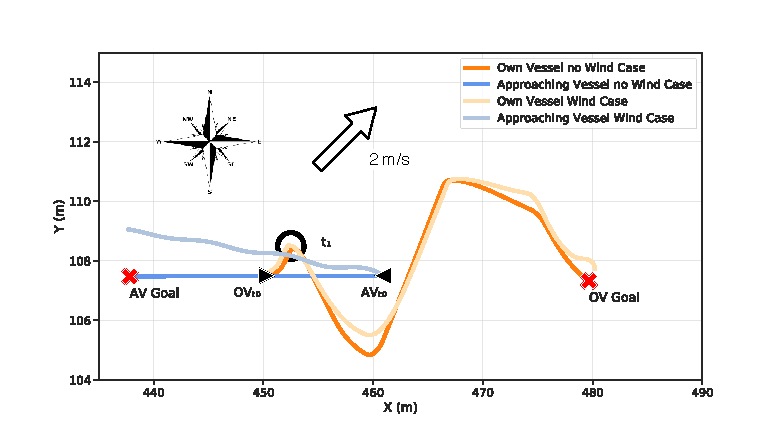
\includegraphics[width=\textwidth]{figs/Chap5/plot_ho_w_vs_wind.pdf}
            \caption{Comparison between the trajectories of the vessels in Wind case and no Wind case in a head-on encounter scenario, both cases use \ac{ATC} A*. Start position for \ac{OV} and \ac{EV} are marked with ">" and "<", while their goals are marked with "x". For the Wind case, the direction of the wind is northeast, represented by an arrow. We can observe that our \ac{ATC} A* kept implying COLREGS compliance even under the influence of wind in this scenario.}
            \label{fig:plot_ho_w_vs_wind}
        \end{figure}
        
        %%%%%%%%%%%%%%%%%%%%%%%%%%%%%%%%%%%%%%
        %% Head-On w vs wo Wind Computational Time
        %
        %% Grammarlly: 100/100
        %%%%%%%%%%%%%%%%%%%%%%%%%%%%%%%%%%%%%%
        Figure \ref{fig:plot_ho_w_vs_wind_CT} shows the computational time measured in seconds over time for wind and no wind cases. We observe that the computational time keep similar and does not seems to be related to the imposed wind influence for this simulation.
        \begin{figure}[H]
            \centering
            \includesvg[width=\textwidth]{figs/Chap5/plot_ho_w_vs_wind_CT.svg}
            \caption{Computational time comparison between Wind case versus no Wind in a head-on encounter.}
            \label{fig:plot_ho_w_vs_wind_CT}
        \end{figure}
        
        %%%%%%%%%%%%%%%%%%%%%%%%%%%%%%%%%%%%%%
        %% Crossing Right w vs wo \ac{ATC}. w vs wo Wind
        %
        %% Grammarlly: 100/100
        %%%%%%%%%%%%%%%%%%%%%%%%%%%%%%%%%%%%%%
        In Figure \ref{fig:plots_cr}, we present the behavior of our system when \ac{OV} encounters another vessel coming from the right side. In Figure \ref{fig:plot_cr_w_vs_wo}, we show the comparison between trajectories with and without ATC and in Figure \ref{fig:plot_cr_w_vs_wo_CT} we can see computational time for each case. As we can see, our method implies COLREGS compliance when avoiding a collision.
        
        In Figure \ref{fig:plot_cr_w_vs_wind} we show the comparison between trajectories with and without wind influence and in Figure \ref{fig:plot_cr_w_vs_wind_CT} we can see computational time for each case. As we can see, once again, our method kept COLREGS-compliant even when disturbed by a maximum of 2.0 m/s wind.
        
        \begin{figure}[H]
        \centering
        
            \begin{subfigure}[b]{0.49\textwidth}
                \centering
                \includesvg[width=\textwidth]{figs/Chap5/plot_cr_w_vs_wo.svg}
                % \caption{Trajectory comparison between \ac{ATC} and no \ac{ATC} cases.}
                \caption{}
                \label{fig:plot_cr_w_vs_wo}
            \end{subfigure}
            \begin{subfigure}[b]{0.49\textwidth}
                \centering
                \includesvg[width=\textwidth]{figs/Chap5/plot_cr_w_vs_wo_CT.svg}
                % \caption{Computation Time. \ac{ATC} and no \ac{ATC} cases.}
                \caption{}
                \label{fig:plot_cr_w_vs_wo_CT}
            \end{subfigure}
            
            \begin{subfigure}[b]{0.49\textwidth}
                \centering
                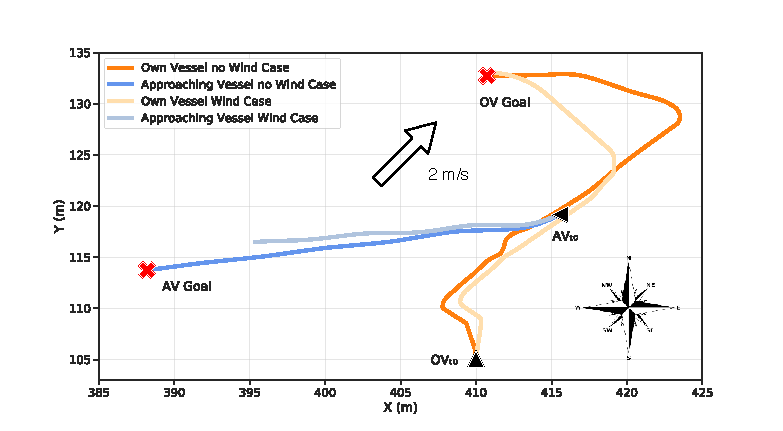
\includegraphics[width=\textwidth]{figs/Chap5/plot_cr_w_vs_wind.pdf}
                % \caption{Trajectory comparison between Wind and no Wind cases}
                \caption{}
                \label{fig:plot_cr_w_vs_wind}
            \end{subfigure}
            \begin{subfigure}[b]{0.49\textwidth}
                \centering
                \includesvg[width=\textwidth]{figs/Chap5/plot_cr_w_vs_wind_CT.svg}
                % \caption{Computation Time. Wind and no Wind cases.}
                \caption{}
                \label{fig:plot_cr_w_vs_wind_CT}
            \end{subfigure}
        
        \caption{Crossing Right Encounter Scenario. Comparison between \ac{ATC} and no \ac{ATC} (a and b), and Wind cases (c and d).}
        \label{fig:plots_cr}
        \end{figure}
        %AMA descobriu pq sem vento a curva mais mais longa do q com vento? parece estar invertido. convem verificar pois vao perguntar isso. nao esta fazendo  sentido.
        
         %AMA pq a posicao final do EV eh diferente com e sem vento ?
         
        In Figure \ref{fig:plot_cr_w_vs_wind}, in the time window we show, the \ac{EV} do not achieve its goal, the wind acts against \ac{EV} motion, reducing the maximun speed.
          
        %%%%%%%%%%%%%%%%%%%%%%%%%%%%%%%%%%%%%%
        %% Overtaking w vs wo \ac{ATC}. w vs wo Wind
        %
        %% Grammarlly: ?/100
        %%%%%%%%%%%%%%%%%%%%%%%%%%%%%%%%%%%%%%
        In Figure \ref{fig:plots_cl}, we present the behavior of our system in an overtaking encounter. In Figure \ref{fig:plot_cl_w_vs_wo} we show the comparison between trajectories with and without \ac{ATC} and in Figure \ref{fig:plot_cl_w_vs_wo_CT} we can see computational time for each case. In an overtaking encounter, \ac{OV} must keep moving ahead, avoiding to generate any other crossing situation while overtaking. In our simulation, \ac{OV} avoids going to \ac{EV} front until it gets near the goal.
        
        In Figure \ref{fig:plot_cl_w_vs_wind} we show the comparison between trajectories with and without wind influence and in Figure \ref{fig:plot_cl_w_vs_wind_CT} we can see computational time for each case. As we can see, our method kept COLREGS-compliant even when disturbed by a maximum of 2.0 m/s wind.
        \begin{figure}[H]
        \centering
        
            \begin{subfigure}[b]{0.49\textwidth}
                \centering
                \includesvg[width=\textwidth]{figs/Chap5/plot_cl_w_vs_wo.svg}
                \caption{Trajectory}
                \label{fig:plot_cl_w_vs_wo}
            \end{subfigure}
            \begin{subfigure}[b]{0.49\textwidth}
                \centering
                \includesvg[width=\textwidth]{figs/Chap5/plot_cl_w_vs_wo_CT.svg}
                \caption{Computation Time}
                \label{fig:plot_cl_w_vs_wo_CT}
            \end{subfigure}
            
            \begin{subfigure}[b]{0.49\textwidth}
                \centering
                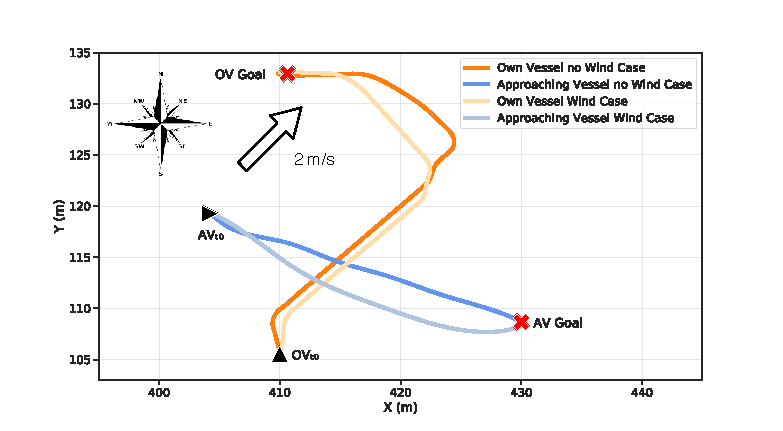
\includegraphics[width=\textwidth]{figs/Chap5/plot_cl_w_vs_wind.pdf}
                \caption{Trajectory}
                \label{fig:plot_cl_w_vs_wind}
            \end{subfigure}
            \begin{subfigure}[b]{0.49\textwidth}
                \centering
                \includesvg[width=\textwidth]{figs/Chap5/plot_cl_w_vs_wind_CT.svg}
                \caption{Computation Time}
                \label{fig:plot_cl_w_vs_wind_CT}
            \end{subfigure}
        
        \caption{Crossing Right Encounter Scenario. Comparing \ac{ATC} versus no \ac{ATC} cases and, with and Wind vs no Wind cases.}
        \label{fig:plots_cl}
        \end{figure}
        %AMA vc nao ia tentar refazer esse resltado p ver se sai essa barriga ?
        %AMA nao eh so para esse caso. esta faltando um paragrafro q discute o resultado. vc esta basicamente so largando as figuras sem nehuma discussao ou explicacao do reaultado obtido. cada caso deve ter uma discussao. nao eh o suficiente somente dizer se conseguiu ou nao realizar.
        %AMA pq tem uma diff no tempo de execucao com e sem vento ? FALTA DISCUSSAO !!!!
      
        
        %%%%%%%%%%%%%%%%%%%%%%%%%%%%%%%%%%%%%%
        %% Overtaking w vs wo \ac{ATC}. w vs wo Wind
        %
        %% Grammarlly: 100/100
        %%%%%%%%%%%%%%%%%%%%%%%%%%%%%%%%%%%%%%
        In Figure \ref{fig:plots_ov}, we present the behavior of our system when \ac{OV} encounters another vessel ahead. 
        %AMA a legenda diz overtaking ... confere os nomes e mantem a coerencia
        In Figure \ref{fig:plot_ov_w_vs_wo} we show the comparison between trajectories with and without ATC and in Figure \ref{fig:plot_ov_w_vs_wo} we can see computational time for each case. As we can see, once again, our method implies COLREGS compliance when avoiding a collision. In Figure \ref{fig:plot_ov_w_vs_wind} we show the comparison between trajectories with and without wind influence and in Figure \ref{fig:plot_ov_w_vs_wind_CT} we can see computational time for each case. 
        \begin{figure}[H]
        \centering
        
            \begin{subfigure}[b]{0.49\textwidth}
                \centering
                \includesvg[width=\textwidth]{figs/Chap5/plot_ov_w_vs_wo.svg}
                \caption{Trajectory}
                \label{fig:plot_ov_w_vs_wo}
            \end{subfigure}
            \begin{subfigure}[b]{0.49\textwidth}
                \centering
                \includesvg[width=\textwidth]{figs/Chap5/plot_ov_w_vs_wo_CT.svg}
                \caption{Computation Time}
                \label{fig:plot_ov_w_vs_wo_CT}
            \end{subfigure}
            
            \begin{subfigure}[b]{0.49\textwidth}
                \centering
                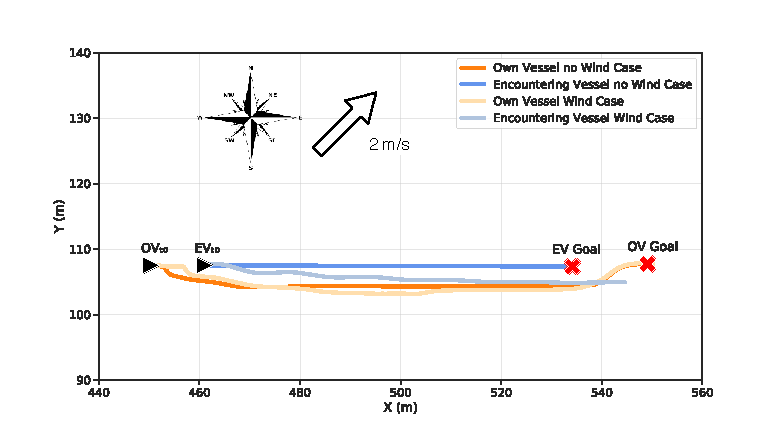
\includegraphics[width=\textwidth]{figs/Chap5/plot_ov_w_vs_wind.pdf}
                \caption{Trajectory}
                \label{fig:plot_ov_w_vs_wind}
            \end{subfigure}
            \begin{subfigure}[b]{0.49\textwidth}
                \centering
                \includesvg[width=\textwidth]{figs/Chap5/plot_ov_w_vs_wind_CT.svg}
                \caption{Computation Time}
                \label{fig:plot_ov_w_vs_wind_CT}
            \end{subfigure}
        
        %% Grammarlly: 98/100
        \caption{Overtaking Encounter Scenario with \ac{ATC}, with and without wind. In \ref{fig:plot_ov_w_vs_wind_CT} we can see a considerable increase in computation time from around 3 minutes until around 4min and 25 second. This happened due to the second limitation discovered in our method. With \ac{ATC} the creation of virtual obstacles can be conflicting with the A* goal location and its neighbors, in this situation the planner is not able to decide the route to be followed and decided to use the last generated speed command until the position of the A* goal location is free. Due to the conflicting position of the created virtual obstacle and local A* goal, the computational time cost achieves great value, since it explored the whole search space and found no solution.}
        \label{fig:plots_ov}
        \end{figure}
        %AMA acho melhor mover as dicussoes p o texto e nao deixar na legenda.
        
        %% Grammarlly: 100/100
        In Table \ref{tab:results}, we summarize the results for the different simulations we have done. In simulation scenarios, we can see that the computational time peak keeps in a range from 0.355 to 0.390 for no \ac{ATC} configuration, from 0.357 to 0.395 for \ac{ATC} configuration and from 0.355 to 0.8852 for Wind configuration. Computation time for no \ac{ATC} and \ac{ATC} are similar since our \ac{ATC} method has a low impact on the A* implementation. With the influence of wind, we see an increase in the computational time peak. For the Overtaking scenario, the influence of wind caused our system to an exhaustive scenario search in the whole search space. 
        %AMA algumas das discussoes q eu reclamei q faltavam estao aqui. Note que eu mencionei ALGUMAS .... 
        % mas vc deve lembrar q o leitor vai ler em ordem. Assim, ele vai ficar com duvidas ate chegar nesse ponto. Nesses casos, vc deve mencionar que, la onde a explicacao tinha q aparecer inicialmente, vc vai discutir tal coisa a seguir.
        
        The average time keeps similar for each scenario encounter, not depending on the configuration (no \ac{ATC}, \ac{ATC}, and Wind). In all cases presented, there is at least a 4.6 ratio between the maximum and average time. The high values reached occur when there is some considerable restriction in the search space, that is when the goal for the local A* conflicts or with the current position of \ac{EV} or with the created virtual obstacle. The average time remains low because the search in 100x100 search space does not demand much effort from the system, considering the platform where we perform the simulation and some execution just needed to generate short and straight paths ahead. Regarding minimum distance, in our simulations, our system kept at least a safe distance of 1.505 meters from \ac{EV}. 
        %AMA e isso eh considerado safe ? de acordo c o que  ou quem ? importante discutir isso.
        %AMA note q na tabela em uma min distance de 0.7 m !!!
        
        
        %\ac{COLREGS} do not specify a specific value for safe distance or a proportion related to \ac{OV}'s size, but for some authors \cite{} \acp{USV} should at least keep a safe distance as the size of the vessel.
        % The average time keeps similar for each scenario encounter, not depending on the configuration (no \ac{ATC}, \ac{ATC}, and Wind) and consumed at least 4.6 times less time. 
        % Regarding minimum distance, in our simulations, our system kept at least a safe distance of 1.505 meters from \ac{EV}. %\ac{COLREGS} do not specify a specific value for safe distance or a proportion related to \ac{OV}'s size, but for some authors \cite{} \acp{USV} should at least keep a safe distance as the size of the vessel.

\begin{table}
\caption{Based on \cite{Lazarowska2017New, Singh2018Constrained, Agrawal2015COLREGS, Candeloro2017Voronoi, Svec2013Dynamics} we made a quantitative evaluation of our planning system measuring computational cost and the minimum distance kept between the vessels during simulations.}
\label{tab:results}
\centering
\begin{tabular}{ccccccc} 
\toprule
\multirow{2}{*}{\begin{tabular}[c]{@{}c@{}}\textbf{Encounter}\\\textbf{Type} \end{tabular}}     & \multirow{2}{*}{\textbf{Case} } & \multicolumn{3}{c}{\textbf{Computational Time (s)} }          & \multirow{2}{*}{\begin{tabular}[c]{@{}c@{}}\textbf{Successful }\\\textbf{Avoidance }\end{tabular}} & \multirow{2}{*}{\begin{tabular}[c]{@{}c@{}}\textbf{Minimum }\\\textbf{Distance (m) }\end{tabular}}  \\ 
\cmidrule[\heavyrulewidth]{3-5}
                                                                                                &                                 & \textbf{Maximum} & \textbf{Average} & \textbf{Std. Variation} &                                                                                                    &                                                                                                     \\ 
\toprule
\multirow{3}{*}{\textbf{Head-On}}                                                               & \textbf{No ATC}                 & 0.369            & 0.074            & 0.081                   & Yes                                                                                                & 4.431                                                                                               \\
                                                                                                & \textbf{ATC}                    & 0.364            & 0.076            & 0.076                   & Yes                                                                                                & 1.599                                                                                               \\
                                                                                                & \textbf{Wind}                   & 0.355            & 0.077            & 0.079                   & Yes                                                                                                & 1.505                                                                                               \\ 
\cline{2-7}
\multirow{3}{*}{\begin{tabular}[c]{@{}c@{}}\textbf{Crossing}\\\textbf{from Right}\end{tabular}} & \textbf{No ATC}                 & 0.390            & 0.050            & 0.098                   & Yes                                                                                                & 5.414                                                                                               \\
                                                                                                & \textbf{ATC}                    & 0.390             & 0.052            & 0.104                   & Yes                                                                                                & 3.264                                                                                               \\
                                                                                                & \textbf{Wind}                   & 0.403            & 0.085            & 0.124                   & Yes                                                                                                & 3.739                                                                                               \\ 
\cline{2-7}
\multirow{3}{*}{\begin{tabular}[c]{@{}c@{}}\textbf{Crossing}\\\textbf{from Left}\end{tabular}}  & \textbf{No ATC}                 & 0.416                 & 0.039                 & 0.096                        &  Yes                                                                                                  & 7.018                                                                                                    \\
                                                                                                & \textbf{ATC}                    & 0.389                 & 0.028                 & 0.080                        & Yes                                                                                                   & 6.274                                                                                                    \\
                                                                                                & \textbf{Wind}                   & 0.400                 & 0.030                 & 0.081                        & Yes                                                                                                   & 5.707                                                                                                    \\ 
\cline{2-7}
\multirow{3}{*}{\textbf{Overtaking}}                                                            & \textbf{No ATC}                 & 0.368            & 0.006            & 0.030                   & Yes                                                                                                & 3.325                                                                                               \\
                                                                                                & \textbf{ATC}                    & 0.357            & 0.018            & 0.022                   & Yes                                                                                                & 3.101                                                                                               \\
                                                                                                & \textbf{Wind}                   & 0.852            & 0.039            & 0.073                   & Yes                                                                                                & 1.787                                                                                               \\
\bottomrule
\end{tabular}
\end{table}
%AMA discuta pq crossing from left tem tempos menores (max, avg, std var)
%AMA discuta p o maximo da ultima linha eh tao maior q os outros
\chapter{Conclusion}
\label{chap:6_Conclusion}

    In this chapter we discuss the results and future work.
    
    \section{Results Discussion}

    In this work, we present a \acl{GNC} (\ac{GNC}) system for autonomous \aclp{USV} (\acp{USV}). Due to the need for vessels that navigate in the water surface to respect \acl{COLREGS} (\ac{COLREGS}), we apply a method of path planning to our system to avoid violating \ac{COLREGS} when a vessel using our system encounters another.

    The system we develop is composed of navigation, control, and guidance modules. The navigation system is responsible for perceiving the state of the surrounding environment and the vessel's state itself. The control system can modify the state of the \ac{USV} and move it. The guidance system defines a path to achieve a goal using the information collected by the navigation system considering the state of the environment and the vessel itself.
    
    Our main contribution was the development and integration of these modules and the adaptation of a technique presented in the literature to make the behavior of a vessel guided by our system respect the \ac{COLREGS}. Our system can react following the \ac{COLREGS} when it finds only one approaching vessel. When finding multiple vessels, our system can generate routes to avoid collision, but the \ac{COLREGS} compliance capacity has not been guaranteed. Another limitation is related to our system, considering that the approaching vessel is of the same type as ours since different categories of vessels imply a change in the \ac{COLREGS} interpretation.
    
    Our solution uses A* to find a path that leads towards the location goal. When a vessel approaches ours, our local planning module reacts and generates \ac{COLREGS}-compliant routes. To generate \ac{COLREGS} compliant routes, we have adapted the solution presented by Agrawal~\etal~\cite{Agrawal2015COLREGS} in our system. When our system detects another vessel in its proximity, it creates a virtual obstacle that restricts the search space of our local planner, excluding positions that would violate \ac{COLREGS}. Thus the local planner is forced to choose a \ac{COLREGS}-compliant route.

    We evaluate the performance of our system regarding the main scenarios of encounter described in \ac{COLREGS}, they are head-on, crossing from the right, crossing from the left, and overtaking. We collected the maximum and average computational time for the execution of our \aclp{ATC} (\ac{ATC}) A* method in each cycle. For all simulated scenarios, our system was able to avoid collision and follow \ac{COLREGS} even with a wind intensity of 2 m/s.

    Our \ac{ATC} A* method has been effective for \ac{COLREGS}-compliance collision avoidance in the scenarios we simulated. Regarding performance, the computational cost is mainly related to our A* implementation. Our A* implementation has several conversions operations between the global and local scope. These operations consist of operations that evaluate the value of each cell in an mxm grid, where m is equal to 100.

    The creation of virtual obstacles with \ac{ATC}, creates indirectly and intermittently an increase in computational time, due to the restriction in the search space. The impact of creating obstacles with \ac{ATC} is low compared to the total cost since the implementation of \ac{ATC} for creating virtual obstacles consists of filling in the values on the local cost map in a wxl area, where w is the local width of our vessel and l  is the distance between the approaching vessel and the corresponding edge of the local cost map. In the worst case, l is 99, since the side of the cost map location is 100, and the \ac{AV} must occupy at least one position of the cost map location. Intermittent behavior occurs because, when an obstacle is created and occupies the same position as the local goal, the local planner extinguishes the entire search area and look backward in the global plan for a valid position goal in the local cost maps.
    
    \section{Future Work}
    
    The main improvements are related to the reduction of computational time, an increase in the maximum speed of the vessel, and a greater variety in possible encounters. Regarding computational time, it is necessary to investigate our implementation of A* to find out if there is any possible improvement that impacts on the total time of execution of our local planner. Another major limitation related to our local planner is the reduced ability to generate velocity commands that allow \ac{USV} to navigate with more than 0.4 m/s. The simulated \ac{USV} model we used in our tests can navigate up to 1.8 m/s. This improvement requires investigation to understand better where the speed restriction is.
    
    Regarding variety in the encounter, our system has the potential to be simulated in an environment with multiple boats. It is necessary to study ways to apply our method based on the creation of virtual obstacles for situations where simultaneous encounters between multiple vessels occur. Perhaps a necessary change is the removal of lethality from virtual obstacles. Currently, the virtual obstacles created are considered impassable by the local planner. In multiple encounters, there is a potential increase in space restriction, where it is not possible to navigate. Therefore, high-cost virtual obstacles could be created for the planner but with the possibility of transposition if it is the only choice to avoid collision.
    
    Related to the encounters variety, we should study ways to consider different categories of vessels found and take this into account when creating virtual obstacles. For example, where our vessel is power-driven and finds a sailing vessel to its left, instead of keeping its course and waiting for the vessel on left to avoid collision, our vessel assumes the responsibility of evading the collision.
    
    Another possible improvement would be to add a ray of cost inflation around the virtual obstacles created. This could prevent the A* method from exploring locations that are neighbors of virtual obstacles, possibly decreasing the computational cost. In the tests performed, the method explored large areas close to the virtual obstacles, due to the heuristic behavior of the algorithm. However, these obstacles could not be overcome, so these nodes were explored but did not lead to the final trajectory.
    
     Regarding real-world tests, we could try to bound the maximum computational time reducing conversions from the local and global planners. So, we could evaluate the performance of our system when running in the embedded computers we have in the vessels of our laboratory. For  real-world tests would be necessary to study how to adequate each of the modules of our system to the hardware available in our vessel.
    
    
%AMA outras coisas q vou te pedir p incluir na distribuicao:  -comments c doxygen style. -script que instala o simulador, aplica todas as depedendencias, e aplica o teu pacote. - distribuicao clean (branches antigos removidos, remover codigo morto, colocar muito comentario (ingles, obvio), revisar se tem variaveis ou funcoes em portugues e renomear, tag da versao estavel) - todos codigos c um cabecalho legal e explicativo - quais sao os parametros q o user pode alterar ? qual eh o impacto de cada parametro ? - melhorar muito o readme principal.- me dar acesso ao https://github.com/Unmanned-Surface-Vehicle. referenciar o lab, a universidade , e a tua tese no readme. verias coisas pequenas q precisam ser melhroadas para q o trbalho nao morra ao final da tua tese.
%DJ: Entendi

%----------------------------------------------------------------
% Aqui vai a bibliografia. Existem dois estilos de citação: use
% 'ppgcc-alpha' para citações do tipo [Abc+] ou [XYZ] (em ordem
% alfabética na bibliografia), e 'ppgcc-num' para citações
% numéricas do tipo [1], [20], etc., em ordem de referência.
%----------------------------------------------------------------
% \bibliographystyle{ppgcc-alpha}
\bibliographystyle{ppgcc-num}
\bibliography{References}

%----------------------------------------------------------------
% Após \appendix, se iniciam os capítulos de Apêndice, com
% numeração alfabética.
%----------------------------------------------------------------
%\appendix
% \include{cap8_appendix}
%\chapter{Meu primeiro apêndice}
%\chapter{My second appendix}

%----------------------------------------------------------------
% Aqui vão os "capítulos" de anexos. Cada anexo deve
% ser considerado um capítulo.
%----------------------------------------------------------------
%\anexos
%\chapter{Meu primeiro anexo}
%\chapter{My second attachment}

% E aqui (para a felicidade de todos) termina o documento.
\end{document}
